\documentclass[pdflatex,11pt]{aghdpl}
% \documentclass{aghdpl}               % przy kompilacji programem latex
% \documentclass[pdflatex,en]{aghdpl}  % praca w języku angielskim
\usepackage[polish]{babel}
\usepackage[utf8]{inputenc}
\usepackage{longtable}
\usepackage{multirow}

% dodatkowe pakiety
\usepackage{hyperref}
\usepackage{enumerate}
\usepackage{listings}
\usepackage{xcolor}
\usepackage{url}
\usepackage{booktabs}
\usepackage{amsmath}

\usepackage{gnuplottex}
\usepackage{graphicx}
\usepackage{color}
\usepackage{multicol}

\usepackage{textgreek}
\usepackage{pifont}
\newcommand{\cmark}{\ding{51}}
\newcommand{\xmark}{\ding{55}}

\usepackage{multicol,caption}
\usepackage{fixltx2e}

\newenvironment{Figure}
  {\par\medskip\noindent\minipage{\linewidth}}
  {\endminipage\par\medskip}

\lstloadlanguages{TeX}

\lstset{
  literate={ą}{{\k{a}}}1
           {ć}{{\'c}}1
           {ę}{{\k{e}}}1
           {ó}{{\'o}}1
           {ń}{{\'n}}1
           {ł}{{\l{}}}1
           {ś}{{\'s}}1
           {ź}{{\'z}}1
           {ż}{{\.z}}1
           {Ą}{{\k{A}}}1
           {Ć}{{\'C}}1
           {Ę}{{\k{E}}}1
           {Ó}{{\'O}}1
           {Ń}{{\'N}}1
           {Ł}{{\L{}}}1
           {Ś}{{\'S}}1
           {Ź}{{\'Z}}1
           {Ż}{{\.Z}}1
}
%---------------------------------------------------------------------------
% Style for Erlang listings

\lstdefinestyle{erlang}{
  belowcaptionskip=1\baselineskip,
  breaklines=true,
  frame=L,
  xleftmargin=\parindent,
  language=C,
  showstringspaces=false,
  showlines=true,
  basicstyle=\footnotesize\ttfamily,
  keywordstyle=\bfseries\color{green!40!black},
  commentstyle=\itshape\color{purple!40!black},
  morekeywords={when, define, module, export, include},
  identifierstyle=\color{blue},
  stringstyle=\color{orange},
  captionpos=b,
  numbers=left,
}
%---------------------------------------------------------------------------

\author{Rafał Studnicki}
\shortauthor{R. Studnicki}

\titlePL{Realizacja podstawowej funkcjonalności maszyny wirtualnej Erlanga dla systemu FreeRTOS}
\titleEN{Implementation of basic features of Erlang Virtual Machine for FreeRTOS}

\shorttitlePL{Podstawowa funkcjonalność Erlanga dla systemu FreeRTOS}
\shorttitleEN{Implementation of basic features of Erlang for FreeRTOS}

\thesistype{Praca dyplomowa magisterska}

\supervisor{dr inż. Piotr Matyasik}

\degreeprogramme{Informatyka}

\date{2014}

\department{Katedra Informatyki Stosowanej}

\faculty{Wydział Elektrotechniki, Automatyki,\protect\\[-1mm] Informatyki i Inżynierii Biomedycznej}

\acknowledgements{}

\setlength{\cftsecnumwidth}{10mm}

%---------------------------------------------------------------------------

\begin{document}

\titlepages

\tableofcontents
\clearpage

%\chapter{Wprowadzenie}
\label{cha:wprowadzenie}

W rozdziale uwzględniono wstępne informacje dotyczące programowania urządzeń wbudowanych, a także opisano dotychczasowe wykorzystanie języków funkcyjnych w programowaniu takich urządzeń.
Opisano w nim także cele oraz zawartość niniejszej pracy.

%---------------------------------------------------------------------------

\section{Programowanie i zastosowanie systemów wbudowanych}
\label{sec:systemyWbudowane}

System wbudowany jest to system komputerowy będący zazwyczaj integralną częścią urządzenia zawierającego elementy sprzętowe i mechaniczne.
W przeciwieństwie do komputerów ogólne przeznaczenia, których celem jest realizacja różnego rodzaju zadań w zależności od potrzeb ich użytkowników, systemy wbudowane realizują tylko jedno, konkretne zadanie.

W obecnych czasach, gdy dąży się do tego, by coraz większa liczba urządzeń powszechnego użytku była "inteligentna" i mogła spełniać swoja zadania całkowicie niezależnie od człowieka, systemy wbudowane wykorzystywane w coraz większej mierze. Przykładami zastosowań systemów wbudowanych mogą być np.:
\begin{itemize}
\item telefony komórkowe;
\item centrale telefoniczne;
\item sterowniki do robotów mechanicznych;
\item sprzęt sterujący samolotami i rakietami;
\item układy sterujące pracą silnika samochodowego, komputery pokładowe;
\item systemy alarmowe, antywłamaniowe, przeciwpożarowe;
\item sprzęt medyczny;
\item sprzęt pomiarowy.
\end{itemize}

Systemy wbudowane najczęściej implementowane są w oparciu o mikrokontrolery, czyli scalone systemy mikroprocesorowe zawierające na jednym, zintegrowanym układzie scalonym oprócz mikroprocesora również pamięć RAM, programu, układy wejścia-wyjścia, układy licznikowe oraz kontrolery przerwań. Zintegrowanie wszystkich tych elementów na jednej płytce pozwala na redukcję rozmiaru i poboru mocy takiego układu.

Spośród architektur projektowania oprogramowania przeznaczonego do programowania urządzeń wbudowanych można wymienić:
\begin{enumerate}
\item kontrola programu w pętli \\
program kontrolowany jest w pojedynczej pętli, wewnątrz której podejmowane są decyzje o sterowaniu elementami sprzętowymi lub programowymi;
\item kontrola programu przez przerwania \\
konkretne zadania programu wywoływane są przez wewnętrzne (np. zegary) lub zewnętrzne (np. odbiór danych z portu szeregowego) przerwania.
Architektura ta często mieszana jest z wykonywaniem programu w pętli. W takim podejściu zadania o wysokim priorytecie wywoływane są przez przerwania, natomiast zadania o niskim priorytecie wykonywane są w pętli;
\item wielozadaniowość z wywłaszczaniem \\
w tego typu systemach pomiędzy kodem programu a mikrokontrolerem znajduje się niskopoziomowe oprogramowanie (jądro) odpowiadające za przydzielanie czasu procesora dla wielu współbieżnych zadań, które mogą mieć różne priorytety wykonania. Planista (\emph{scheduler}) decyduje także w którym momencie powinno zostać obsłużone przerwanie;
\item wielozadaniowość bez wywłaszczania \\
tego rodzaju architektura jest bardzo podobna do wielozadaniowości z wywłaszczaniem, jednak jądro nie dokonuje samodzielnych decyzji o przerwaniu wykonywania któregoś ze współbieżnych zadań lecz pozostawia tę decyzję programiście;
\item mikrojądro \\
jest rozszerzeniem systemów obsługujących wielozadaniowość bez wywłaszczania lub z wywłaszczaniem poprzez dodanie np. zarządzania pamięcią, mechanizmów synchronizacji czy komunikacji pomiędzy współbieżnymi zadaniami do funkcjonalności jądra. Przykładami mikrojąder mogą być np. FreeRTOS, Enea OSE czy RTEMS;
\item jądro monolityczne
do funkcjonalności jądra dodaje funkcjonalności zapewniające komplet komunikacji z peryferiami systemu dodające do funkcjonalności np. system plików, stos TCP/IP do komunikacji sieciowej, czy sterowniki obsługi urządzeń zewnętrznych.
Spośród systemów z jądrami monolitycznymi można wymienić takie systemy jak Embedded Linux czy Windows CE.
\end{enumerate}

Można zauważyć, że wymienione architektury zostały uporządkowane względem złożoności projektowanego systemu, ale także pod względem złożoności występującego elementu pośredniego pomiędzy programowanym fizycznym urządzeniem a oprogramowaniem. Wraz ze wzrostem złożoności systemu rosną również wymagania sprzętowe konieczne do uruchomienia danego systemu, maleje jednak bezpośredni poziom kontroli programisty nad realizacją wymagań czasu rzeczywistego.
W niniejszej pracy rozważane będą sposoby implementacji oprogramowania na systemy wbudowane w oparciu o mikrojądra.

%---------------------------------------------------------------------------

\section{Wykorzystanie Erlanga w programowaniu systemów wbudowanych}
\label{sec:jezykiFunkcyjne}

Jim Gray w pracy \emph{Why Do Computers Stop And What Can Be Done About It?} \cite{Gray85whydo} na podstawie obserwacji procesu projektowania i budowy sprzętu wchodzącego w skład systemów komputerowych sformułował pewne postulaty dotyczące implementacji oprogramowania odpornego na błędy.
Były one następujące:
\begin{enumerate}
\item oprogramowanie powinno być modularne, co powinno zostać zapewnione przez wyabstrahowanie logiki w procesach. Komunikacja między procesami powinna zostać zapewniona przez mechanizm przesyłania wiadomości;
\item propagacja błędów powinna być powstrzymywana tak szybko jak to tylko możliwe (\emph{fail-fast});
\item logika wykonywana przez procesy powinna być zduplikowana w całym systemie tak, aby możliwe było jej wykonanie pomimo błędu sprzętowego lub tymczasowego błędu innego modułu;
\item powinien zostać zapewniony mechanizm transakcyjny pozwalający na zachowanie spójności danych;
\item powinien zostać zapewniony mechanizm transakcyjny, który w połączeniu z duplikacją procesów ułatwi obsługę wyjątków i tolerowanie błędów oprogramowania.
\end{enumerate}

Obserwacje te były motywacją dla czwórki inżynierów z firmy Ericsson AB - Bjarne Dackera, Joe Armstrona, Mike'a Williams i Roberta Virdinga do stworzenia nowej platformy spełniającej powyższe wymagania i w oparciu o którą możliwe byłoby tworzenie projektów wewnątrz firmy.
Jak się później okazało, do zaspokojenia wszystkich wymienionych potrzeb konieczne było stworzenie nowego, dedykowanego języka programowania - Erlang, wraz z zestawem bibliotek - OTP (Open Telecom Platform).

Rozwiązanie to zapewniało realizację powyższych postulatów poprzez następujące cechy charakterystyczne:
\begin{enumerate}
\item izolowane, lekkie i możliwe do szybkiego uruchomienia procesy, które nie mogą bezpośrednio oddziaływać na inne uruchomione w systemie;
\item współbieżne uruchomienie procesów;
\item możliwość wykrywania błędów w jednym procesie przez drugi (monitorowanie procesów);
\item możliwość zidentyfikowania błędu i podjęcia odpowiedniej akcji w jego efekcie;
\item możliwość podmiany kodu uruchamianego programu w locie;
\item niezawodna baza danych (mnesia wchodząca w skład OTP).
\end{enumerate}

Należy zaznaczyć, że celem przyświacającym twórcom języka od samego początku było zastosowanie go w urządzeniach w budowanych, jak np. w centrali telekomunikacyjnej Ericsson AXD301, która pozostaje tego typu urządzeniem o największej liczbie sprzedanych egzemplarzy.

W tym miejscu nie można jednak zapomnieć o tym, że język ten został zaprojektowany dla systemów o miękkich wymaganiach czasu rzeczywistego. Systemy tego typu charakteryzują się tym, że oczekiwane czasy odpowiedzi w tym systemie są rzędu milisekund a odstępstwa od oczekiwanego czasu odpowiedzi powodują tylko spadek jakości usług danego systemu. W przeciwieństwie do tego, systemy o twardych wymaganiach czasu rzeczywistego uznaje się w takich sytuacjach za niefunkcjonujące.


Dystrybucja maszyny wirtualnej Erlanga BEAM (Bjorn/Bogdan Erlang Abstract Machine), która utrzymywana jest przez firmę Ericsson AB umożliwia uruchomienie jej w trybie wbudowanym na takich systemach operacyjnych jak VxWorks czy Embedded Solaris. Pierwszy z nich jest systemem operacyjnym czasu rzeczywistego, jednak maszyna wirtualna została przeniesiona na ten system tylko w zakresie pozwalającym na uruchomienie na niej centrali telekomunikacyjnej, a jej uruchomienie wymaga 32 MB pamięci RAM i 22 MB przestrzeni dyskowej.
Z kolei uruchomienie Erlang/OTP na systemie Embedded Solaris wymaga 17 MB pamięci RAM i 80 MB przestrzeni dyskowej.
Szczegóły dotyczące wersji maszyny wirtualnej na te systemy operacyjne mogą zostać znalezione w dokumentacji Erlang/OTP \cite{ErlangVxWorks}.


Oprócz tego, aktualnie rozwijanym, otwartym projektem związanym z uruchomieniem Erlanga na systemach wbudowanych jest Embedded Erlang. Powstający on przy współpracy firmy Erlang Solutions Ltd. Skupia się on jednak na uruchomieniu maszyny wirtualnej na Raspberry Pi oraz Paralleli, które wymagają pełnej dystrybucji systemu operacyjnego Linux. Szczegóły dotyczące projektu można znaleźć na stronie http://www.erlang-embedded.com.


Zatem wymagania, jakich potrzebują zarówno wymienione przeniesienia (\emph{porty}) maszyny BEAM oraz Embedded Erlang są zdecydowanie zbyt wysokie w porównaniu do specyfikacji sprzętowych rozważanych w niniejszej pracy.


W momencie powstawania pracy firma Ericsson AB była w trakcie implementacji maszyny wirtualnej Erlanga dla systemu operacyjnego czasu rzeczywistego Enea OSE. System ten abstrahuje logikę implementowanego oprogramowania w izolowanych procesach, komunikujących się między sobą poprzez wiadomości (\emph{actor model}). Poziom zgodności z filozofią Erlanga sprawia, że OSE wydaje się być idealnym systemem do implementacji maszyny wirtualnej dla tego języka. Pozostaje on jednak produktem zamkniętym.

Innym projektem godnym uwagi jest Grisp, autorstwa Peera Stritzingera, będący portem maszyny wirtualnej Erlanga dla mikrojądra RTEMS \cite{Stritzinger2013}. W momencie pisania pracy Grisp również pozostaje w trakcie rozwoju, jednak tak jak i maszyna dla systemu OSE pozostaje projektem zamkniętym.
%---------------------------------------------------------------------------

\section{Cele pracy}
\label{sec:celePracy}

Oczekiwanym efektem niniejszej pracy jest implementacja funkcjonalności systemu uruchomieniowego dla funkcyjnego, współbieżnego języka programowania Erlang dla systemu operacyjnego czasu rzeczywistego FreeRTOS.
Zakres implementacji powinien pozwolić na uruchomienie kodu pośredniego (bajtkodu) maszyny wirtualnej Erlanga skompilowanego przez kompilator maszyny wirtualnej BEAM na mikrokontrolerach o ograniczonych zasobach sprzętowych (jak np. mikrokontroler z serii LPC17xx, mający 512kB pamięci flash i 64kB pamięci RAM).

Sposób implementacji powinien pozwolić na uruchamianie programów w taki sposób, by możliwe było spełnienie przynajmniej pierwszych czterech cech charakterystycznych dla języka Erlang z podrozdziału \ref{sec:jezykiFunkcyjne}. Punkt 6. został na tym etapie pominięty, gdyż integracja systemu FreeRTOS z obsługą systemu plików leży poza zakresem pracy. Udostępnienie interfejsów sieciowych oraz możliwość korzystania z mechanizmu klastra Erlanga (\emph{Distributed Erlang}) również nie jest jednym z celów niniejszej pracy.

Celem pracy jest zatem umożliwienie implementacji oprogramowania uruchamianego w ramach systemach wbudowanych o miękkich wymaganiach czasu rzeczywistego, przy pomocy języka programowania Erlang. 

%---------------------------------------------------------------------------

\section{Zawartość pracy}
\label{sec:zawartoscPracy}
%\chapter{System operacyjny FreeRTOS}
\label{cha:freertos}

W niniejszym rozdziale opisano architekturę systemu (mikrojądra) FreeRTOS wraz ze sposobem, w jaki
poszczególne funkcjonalności mogą być przydatne w implementacji maszyny wirtualnej Erlanga dedykowanej
dla tego systemu.

%---------------------------------------------------------------------------
\section{Wprowadzenie}
\label{sec:rtosWprowadzenie}

Podstawową częścią każdego systemu operacyjnego jest jego jądro
FreeRTOS jest mikrojądrem, umożliwiającym tworzenie aplikacji czasu rzeczywistego (zarówno o miękkich jak i twardych wymaganiach) przeznaczonych na systemy wbudowane. 

%---------------------------------------------------------------------------
\section{Zadania i planista (\emph{scheduler})}
\label{sec:rtosScheduler}

%---------------------------------------------------------------------------
\section{Kolejki}
\label{sec:rtosKolejki}

%---------------------------------------------------------------------------
\section{Przerwania}
\label{sec:rtosPrzerwania}

%---------------------------------------------------------------------------
\section{Zarządzanie zasobami}
\label{sec:rtosZasoby}

%---------------------------------------------------------------------------
\section{Zarządzanie pamięcią}
\label{sec:rtosPamiec}

%---------------------------------------------------------------------------
\section{FreeRTOS i LPC17xx}
\label{sec:rtosLPC}

Mikrokontroler LPC17xx jest jednym z systemów, na który przeniesiony został mikrojądrem FreeRTOS.

%---------------------------------------------------------------------------
\section{Podsumowanie}
\label{sec:rtosPodsumowanie}
%\chapter{Język programowania Erlang}
\label{cha:erlang}

%---------------------------------------------------------------------------
\section{Wprowadzenie}
\label{sec:erlangWprowadzenie}
%---------------------------------------------------------------------------
\section{System typów danych}
\label{sec:erlangTypy}

Tu będzie coś o typach danych w Erlangu i ich reprezentacji w pamięci.
%---------------------------------------------------------------------------
%---------------------------------------------------------------------------
\chapter{Zaimplementowane elementy maszyny wirtualnej}
\label{cha:maszyna}

Maszyna wirtualna jest warstwą abstrakcji uruchamianą pod kontrolą pewnego systemu operacyjnego.
Powinna ona emulować fizyczny procesor w taki sam sposób niezależnie od systemu operacyjnego czy fizycznej architektury na jakiej została uruchomiona.
Dzięki temu możliwe jest uruchomienie tego samego kodu, nazywanego kodem pośrednim, przystosowanego do architektury maszyny wirtualnej, pod kontrolą różnych systemów operacyjnych i na różnych architekturach sprzętowych.

Wśród funkcjonalności wirtualnego procesa, które powinna implementować maszyna wirtualna dowolnego języka można wymienić:
\begin{itemize}
\item struktury danych, przy pomocy których opisane są instrukcje i ich argumenty;
\item stos, wykorzystywany do wywołań funkcji;
\item wskaźnik kolejnej instrukcji do wykonania;
\item interpreter kodu pośredniego, pobierający kolejną instrukcję do wykonania, dekodujący jej argumenty i wykonujący ją.
\end{itemize}

W rozdziale wymieniono elementy maszyny wirtualnej Erlanga, które zaimplementowano w pracy, tak aby powyższy zbiór funkcjonalności zapewniał możliwość wykonywania kodu modułów skompilowanych przy użyciu kompilatora Erlanga w wersji R16.
Opis poszczególnych elementów zawiera wyjaśnienie ich sposobu działania, ich roli w maszynie wirtualnej, a także porównania
funkcjonalności do maszyny wirtualnej BEAM.

Wszystkie opisywane funkcjonalności zostały zaimplementowane w języku C, w oparciu o kod źródłowy maszyny wirtualnej BEAM, który opublikowany jest na licencji \emph{Erlang Public License} \cite{epl}.

%---------------------------------------------------------------------------
\section{Moduł ładujący kod (\emph{loader})}
\label{sec:maszynaLoader}

Moduł opisany w niniejszym podrozdziale został zaimplementowany w pliku źródłowym \texttt{beam\_load.c}.

Podstawowym zadaniem \emph{loadera} jest wykonanie zestawu operacji po których będzie możliwe wykonanie kodu programu, zawartego w pliku będącym efektem kompilacji modułu w języku Erlang, z~poziomu interpretera kodu pośredniego w maszynie wirtualnej.
W maszynie BEAM źródłem plików binarnych może być system plików systemu operacyjnego lub inny węzeł Erlanga znajdujący się w tym samym klastrze. Aby pliki te mogły być wykonywane na maszynie zaimplementowanej w ramach pracy, która nie obsługuje ani systemu plików ani protokołu klastrowania, muszą one ulec przetworzeniu i zostać wkompilowane w kod maszyny wirtualnej. Dokonywane jest to za pomocą narzędzia opisanego w~dodatku \ref{cha:builder}.

Zawartość pliku, który poddawany jest przetwarzaniu w module została szczegółowo opisana w dodatku \ref{cha:erlangKompilacja}, który ze względu na brak oficjalnej dokumentacji powstał na potrzeby niniejszej pracy.

Aby możliwe było wykonywanie kodu pośredniego przez maszynę wirtualną, konieczne jest wykonanie następujących kroków:
\begin{itemize}
\item załadowanie lokalnej tablicy atomów (fragment \texttt{Atom}) do globalnej tablicy atomów (por. \ref{sub:maszynaTablicaAtomow});
\item załadowanie lokalnej tablicy eksportowanych funkcji (fragment \texttt{ExpT}) do jej globalnego odpowiednika (por. \ref{sub:maszynaTablicaEksportow});
\item sparsowanie wyrażeń w postaci \emph{External Term Format}, umieszczonych we fragmencie \texttt{LitT} i~umieszczenie ich w pamięci o globalnym dostępie (globalnej stercie);
\item wyszukanie w globalnej tablicy eksportów funkcji zewnętrznych używanych przez moduł (fragment \texttt{ImpT});
\item podstawienie wyrażeń rozpoznawanych globalnie (por. \ref{sec:maszynaTypy}) za wyrażenia lokalne, opisane w podrozdziale \ref{sec:opsTypes} we fragmencie \texttt{Code}. Do rozważanych wyrażeń należą: atomy, etykiety lokalnych funkcji, odnośniki do funkcji znajdujących się w innych modułach oraz wyrażenia umieszczone na globalnej stercie;
\item podstawienie za numery operacji z sekcji \texttt{Code} (opisane w podrozdziale \ref{sec:opsOps}) wskaźników do odpowiedniej sekcji interpretera kodu maszynowego wykonującemu daną instrukcję (por. \ref{sec:maszynaInterpreter}).
\end{itemize}

\emph{Loader} maszyny wirtualnej BEAM wykonuje jeszcze jeden bardzo istotny krok, którego nie wykonuje maszyna zaimplementowana w pracy. Jest nim zastosowanie gramatyki modyfikującej w bardzo istotny sposób kod maszynowy zawarty w pliku binarnym. Gramatykę tę można znaleźć w pliku \texttt{ops.tab} w kodzie źródłowym maszyny BEAM. Wynikowy zestaw instrukcji, odpowiadający instrukcjom faktycznie interpretowanym przez BEAM, jest dużo bardziej obszerny od zestawu który może zostać wygenerowany przez kompilator. Motywacją do zmiany kodu maszynowego w~ten sposób jest m.in. optymalizacja czasu wykonania często występujących po sobie operacji. W przeciwieństwie do oryginalnej maszyny wirtualnej, interpreter zawarty w niniejszej maszynie wirtualnej dokonuje bezpośredniej interpretacji opkodów, które znajdują się w pliku binarnym z kodem pośrednim.

%---------------------------------------------------------------------------
\section{Tablice}
\label{sec:maszynaTablice}

Tablice opisane w tym podrozdziale zostały zaimplementowane w plikach \texttt{hash.c}, \texttt{index.c}, \texttt{atom.c} oraz \texttt{export.c}.

Biorąc pod uwagę modułowy charakter aplikacji napisanych w języku Erlang, maszyna wirtualna musi posiadać pewien mechanizm pozwalający na utrzymywanie globalnego stanu systemu w zależności od aktualnie załadowanych modułów.

Strukturą danych przeznaczoną do tego celu jest tablica z haszowaniem wspomagana przez tablicę indeksów. Połączenie tych dwóch struktur umożliwia wstawienie nowego elementu oraz sprawdzenie jego indeksu w czasie stałym (konieczne jest wyliczenie skrótu). W takim samym czasie (nie jest do tego jednak konieczne wyliczanie skrótu) możliwe jest znalezienie obiektu znając jego indeks. Co więcej, w~reprezentacji kodu maszynowego posługiwanie się indeksami obiektów trywializuje ich porównywanie czy pobieranie ich wartości w trakcie jego wykonywania.

Wybór takiej struktury danych ma więc charakter optymalizacyjny. W maszynie wirtualnej tablicowanymi obiektami są: atomy i eksportowane funkcje. Maszyna wirtualna BEAM dodatkowo tablicuje również moduły, gdzie przechowywane są informacje o wskaźnikach do początku kodu modułu w dwóch wersjach: nowej i starej, które mogą działać w maszynie wirtualnej niezależnie od siebie. Ponieważ jednak maszyna rozważana w pracy w obecnej fazie rozwoju nie zapewnia możliwości dynamicznego ładowania modułów, implementacja tej struktury nie było konieczne.

Na rysunku \ref{fig:atomtable} przedstawiono sposób w jaki wewnątrz maszyny wirtualnej przechowywane są stablicowane dane.  Przykład ten dotyczy dwuelementowej tablicy atomów, które były do niej wstawiane w~kolejności: \texttt{erlang}, \texttt{+}. Strzałki na diagramie reprezentują przechowywanie wskaźników na struktury atomów przez tablice: z haszowaniem i indeksów.

\begin{figure}[h]
\centerline{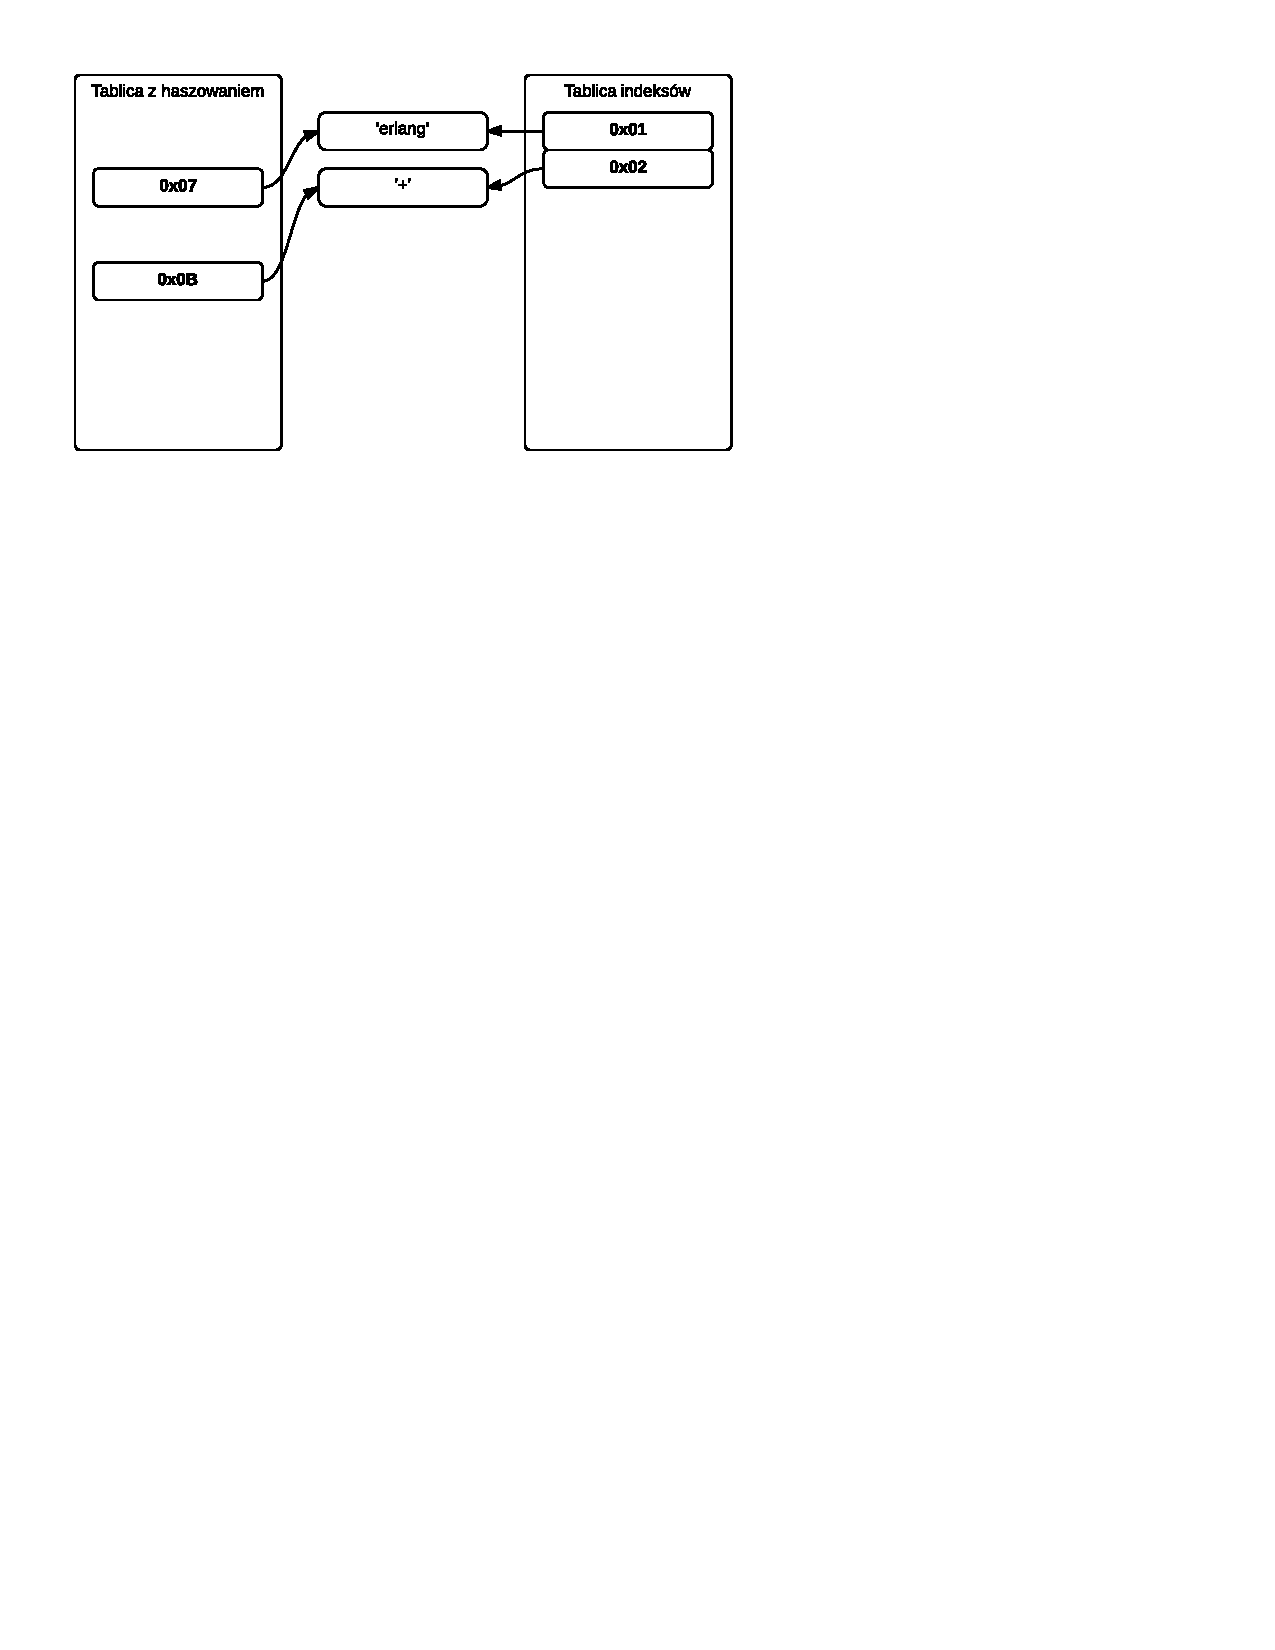
\includegraphics[scale=1, clip, trim=10mm 200mm 90mm 10mm]{atom_table}}
\caption{Przykład przechowywania danych stablicowanych danych wewnątrz maszyny wirtualnej.}
\label{fig:atomtable}
\end{figure}

W maszynie BEAM, w przypadku uruchomionych dużych systemów, powyższe struktury danych mogą zawierać bardzo dużą liczbę elementów, nawet rzędu kilkudziesięciu tysięcy. Zupełnie inaczej sytuacja wygląda w niniejszej maszynie wirtualnej ze względu na jej przeznaczenie, którym są systemy wbudowane i wynikające z tego restrykcyjne limity dostępnej pamięci RAM. Rozmiary tablic nie powinny zatem przekraczać liczby elementów wyrażonej w setkach atomów czy funkcji eksportowanych. Niemniej jednak, ze względu na możliwość uruchomienia systemu FreeRTOS na mikrokontrolerach o różnych parametrach, pozostawiono możliwość zdefiniowania maksymalnej liczby elementów, jakie mogą zostać wstawione do tablic. Zaimplementowano również mechanizmy automatycznego rozszerzania tablic wraz ze wzrostem liczby elementów, w celu optymalizacji pamięci zajmowanej przez tablice.

Ważną cechą charakterystyczną tablic w maszynie wirtualnej jest również fakt, że raz wstawionego do nich obiektu nie można z niej usunąć. W kontekście maszyny wirtualnej rozważanej w pracy ta cecha nie ma większego znaczenia, gdyż obecnie nie umożliwia ona dynamicznego ładowania modułów po jej uruchomieniu. Jednak w przypadku maszyny BEAM nie należy zapominać o tej cesze np. w sytuacji, gdy program generuje atomy w sposób dynamiczny. Tablica atomów w BEAM może przechowywać aż 1048576 atomów, należy jednak mieć na uwadze to, że próba dodania atomu do pełnej już tablicy zakończy się zakończeniem procesu maszyny wirtualnej.

%---------------------------------------------------------------------------
\subsection{Tablica atomów}
\label{sub:maszynaTablicaAtomow}

Funkcja skrótu dla atomów (ich reprezentacji w postaci napisu) używana w maszynie wirtualnej to \emph{hashpjw} \cite{Aho1986}. Jest to funkcja o bardzo dobrym rozkładzie wartości skrótu dla napisów, jednak wartość zwracana przez oryginalną funkcję jest 32-bitowa.

W celu ograniczenia pamięci zajmowanej przez tablice w maszynie wirtualnej rozważanej w pracy, funkcja haszująca została zmodyfikowana tak, aby zwracała wynik 8-bitowy. Ze względu na duże różnice w rozmiarach tablic pomiędzy rozważaną maszyną a BEAM zmniejszenie długości skrótu zwracanego z funkcji haszującej nie będzie miało wpływu na liczbę kolizji w tablicy z haszowaniem. 

Źródłem atomów w tablicy są atomy zdefiniowane w samej maszynie wirtualnej oraz atomy pochodzące z ładowanych modułów. Atomy zdefiniowane ładowane są do tablicy w trakcie uruchamiania maszyny wirtualnej w określonej kolejności, co za tym idzie atomy te mają z góry ustalony i znany indeks, co jest wykorzystywane np. przy definicji funkcji wbudowanych w maszynę wirtualną (por. \ref{sec:maszynaBIF}). Z kolei indeksy atomów, które pochodzą z ładowanych modułów, a nie zostały wcześniej zdefiniowane, przydzielane są w~kolejności ładowania modułów i występowania atomów w tablicach atomów modułów. Równość dwóch atomów oznacza zawsze równość ich indeksów w globalnej tablicy atomów i na odwrót, niezależnie od źródła ich pochodzenia ani momentu załadowania modułu do maszyny wirtualnej.

%---------------------------------------------------------------------------
\subsection{Tablica eksportowanych funkcji}
\label{sub:maszynaTablicaEksportow}

Funkcja skrótu dla eksportowanych funkcji ma wartość $M \cdot F+A$, gdzie $M$ to indeks w tablicy atomów dla nazwy modułu z którego eksportowana jest funkcja, $F$ to indeks w tablicy atomów dla nazwy eksportowanej funkcji, a $A$ to arność tej funkcji.

Wpisy w tablicy eksportowanych funkcji pochodzą z modułów załadowanych do maszyny wirtualnej, dla funkcji które zostały zdefiniowane w lokalnej tablicy eksportów dla danego modułu. W takiej sytuacji w tablicy eksportów przechowywany jest wskaźnik na miejsce w pamięci, w którym znajduje się pierwsza instrukcja funkcji. Interpreter, wykonując kod używa indeksu do odczytania adresu tej instrukcji, a następnie wykonuje skok do tego miejsca pamięci i kontynuuje wykonywanie kodu, po uprzednim zapisaniu adresu powrotu.

Elementy tablicy mogą pochodzić również z wbudowanych funkcji (por. \ref{sec:maszynaBIF}). W tym przypadku, tablica eksportów zawiera wskaźnik do funkcji w języku C, zaimplementowanej jako część maszyny wirtualnej, która zostanie wykonana przez interpreter.

Ponieważ równość indeksów w tablicy eksportów jest równoważna z równością trójek $\lbrace\text{moduł},\text{funkcja},\text{arność}\rbrace$, w sytuacji dynamicznej podmiany kodu nie jest konieczna zmiana indeksu w załadowanym do pamięci kodzie maszynowym, a tylko odpowiednia zmiana struktury znajdującej się pod tym indeksem.

%---------------------------------------------------------------------------
\section{Typy danych}
\label{sec:maszynaTypy}

Erlang jest językiem programowania o dynamicznym, lecz silnym typowaniu. Oznacza to, że każda zmienna, po przypisaniu do niej wartości ma ustalony konkretny typ danych, którego nie można zmienić. Niemożliwe jest również rzutowanie zmiennej na inny typ danych - konwersja do innego typu musi zostać wykonana jawnie a nowa zmienna zajmuje w takiej sytuacji inne miejsce w~pamięci programu.

Wszystkie wyrażenia rozpoznawane przez interpreter kodu maszynowego Erlanga zapisane są w~postaci wyrażenia takiego samego typu, z punktu widzenia języka C, o długości równej słowu maszynowemu dla danej architektury.
W celu rozróżnienia typów zmiennych w pamięci programu, w maszynie wirtualnej wprowadzony został mechanizm \textbf{tagowania}, czyli oznaczania w różny sposób zmiennych w~pamięci, w~zależności od ich typu. Mechanizm ten został zaprojektowany w taki sposób, aby dodatkowy rozmiar w pamięci przeznaczony dla typu był jak najmniejszy. Sposób jego działania został przedstawiony w niniejszym podrozdziale.

\subsection{Wartości bezpośrednie a pośrednie}
\label{sub:typyTypy}

Podstawowy podział typów danych wewnątrz maszyny wirtualnej Erlanga wynika ze względu na sposób dostępu do danych. 

Jeżeli dana może zostać przechowana na odpowiednio małym obszarze pamięci, czyli w jednym słowie maszynowym (w przypadku niniejszej maszyny są to 32 bity) z uwzględnieniem tagu oznaczającego typ to dane tego typu nazywane są wartościami bezpośrednimi (\textbf{IMMED}). Aby dokonać tagowania lub odczytania wartości ze zmiennej tego typu wystarczy wykonać jedną operację przesunięcia bitowego.

Przeciwieństwem danych bezpośrednich są dane pośrednie, które mogą przybrać postać listy (\textbf{CONS}) lub typu opakowanego (\textbf{BOXED}).
Wyrażenia oznaczone tagiem dla jednego z tych typów przechowują fizyczny wskaźnik na miejsce w~pamięci, gdzie znajdują się dla nich właściwe dane.
Przy tagowaniu wskaźników wykorzystany został fakt, że bloki pamięci alokowane przez maszynę wirtualną są zawsze wielokrotnością całego słowa maszynowego.
Co za tym idzie dwa najmniej znaczące bity wskaźnika, na maszynie uruchomionej w architekturze 32-bitowej lub wyższej będą zawsze zerami co można wykorzystać do przechowania dodatkowej, dwubitowej, informacji. W tym wypadku jest to tag rozróżniający wskaźniki na listy od wskaźników na typy opakowane oraz od pozostałych wyrażeń.

Tabela \ref{table:primaryTags} prezentuje sposób tagowania ww. typów danych.
Tagi dla poszczególnych typów danych zostały w zapisie słowa maszynowego pogrubione.

Na przykład do przechowania wskaźnika do pierwszego elementu listy, znajdującego się pod adresem 128, w pamięci zapisane zostane wyrażenie:
$$\texttt{10000000} \vee \texttt{\textbf{01}} = \texttt{00000000 00000000 00000000 100000\textbf{01}}$$

Do odczytania wartości wskaźnika wystarczy więc wyzerowanie dwóch najmniej znaczących bitów wyrażenia:
$$\texttt{00000000 00000000 00000000 100000\textbf{01}} \wedge  \lnot(\texttt{11}) = \texttt{10000000}$$ 

\begin{longtable}{|c|p{4cm}|p{8cm}|}
\hline

Typ danych & Słowo maszynowe (binarnie) & Opis \\
\endfirsthead
\hline

\textbf{IMMED} & \texttt{IIIIIIII IIIIIIII IIIIIIII IIBBTT\textbf{11}} &
\vspace{-8mm}
\begin{itemize}
\item bity \texttt{T} budują konkretny tag (por. \ref{sub:typyImmediates}) typu bezpośredniego;
\item bity \texttt{I} oznaczają wartość przechowywaną przez wyrażenie, która w zależności od rozmiaru tagu może mieć 26 lub 28 bitów;
\item bity \texttt{B} mogą być dwoma najbardziej znaczącymi bitami tagu lub dwoma najmniej znaczącymi bitami przechowywanej wartości, w zależności od typu.
\end{itemize}  
\vspace{-8mm}
\\
\hline
\textbf{CONS} & \texttt{PPPPPPPP PPPPPPPP PPPPPPPP PPPPPP\textbf{01}} &
\vspace{-8mm}
\begin{itemize}
\item bity \texttt{P} są 30 najbardziej znaczącymi bitami wskaźnika do wyrażenia stanowiącego pierwszy element listy, dwa najmniej znaczące bity zawsze będą zerami dlatego mogą zostać nadpisane przez tag.
\end{itemize}  
\vspace{-8mm}
\\
\hline
\textbf{BOXED} & \texttt{PPPPPPPP PPPPPPPP PPPPPPPP PPPPPP\textbf{10}} &
\vspace{-8mm}
\begin{itemize}
\item bity \texttt{P} są 30 najbardziej znaczącymi bitami wskaźnika do nagłówka identyfikujące typ i~rozmiar opakowanych danych, w tym przypadku również dwa najmniej znaczące bity zawsze będą zerami.
\end{itemize}  
\vspace{-8mm}
 \\
\hline
\caption{Rozróżnienie tagów ze względu na sposób dostępu do danych} 
\label{table:primaryTags} \\
\end{longtable}

\subsection{Wartości bezpośrednie}
\label{sub:typyImmediates}

Wartości bezpośrednie (\textbf{IMMED}) mogą być przechowywane przez różne typy danych, dla których przewidziano dodatkowe 2 lub 4 bity na tag. Tabela \ref{table:secondaryImmed} podsumowuje wszystkie zaimplementowane w~maszynie wirtualnej opisywanej w~pracy typy zawierające wartości bezpośrednie.

\begin{longtable}{|c|p{4cm}|p{8cm}|}
\hline

Typ danych & Słowo maszynowe (binarnie) & Opis \\
\endfirsthead
\hline

\textbf{PID} & \texttt{IIIIIIII IIIIIIII IIIIIIII IIII\textbf{0011}} & Wartością przechowywaną przez wyrażenie tego typu jest indeks procesu w tablicy procesów w maszynie wirtualnej (por. \ref{sec:maszynaProcesy}).\\
\hline
\textbf{SMALL\_INT} & \texttt{IIIIIIII IIIIIIII IIIIIIII IIII\textbf{1111}} & Przechowywaną wartością jest liczba całkowita (ze znakiem), którą można zapisać na maksymalnie 28 bitach w pamięci. \\
\hline
\textbf{ATOM} & \texttt{IIIIIIII IIIIIIII IIIIIIII II\textbf{001011}} & Wartością przechowywaną jest indeks atomu w tablicy atomów (por. \ref{sub:maszynaTablicaAtomow}). Dzięki takiemu zapisowi porównanie dwóch dowolnych atomów sprowadza się do porównania dwóch 32-bitowych liczb.  \\
\hline
\textbf{NIL} & \texttt{00000000 00000000 00000000 00\textbf{111011}} & Przechowywaną wartością jest zawsze zero. Wyrażenie to służy do oznaczania końca listy. \\
\hline
\caption{Rozróżnienie tagów dla danych bepośrednich} 
\label{table:secondaryImmed} \\
\end{longtable}

Na przykład atom mający indeks $2_{10} = 10_{2}$ w tablicy atomów w pamięci będzie zapisany w postaci:
$$(\texttt{10} \ll 6) \vee \texttt{\textbf{001011}} = \texttt{00000000 00000000 00000000 10\textbf{001011}}$$

Do odczytania indeksu atomu wystarczy zatem wykonać operację przesunięcia bitowego w prawo:
$$\texttt{00000000 00000000 00000000 10\textbf{001011}} \gg 6 = \texttt{10}$$

\subsection{Listy}
\label{sub:typyLists}

Listy są jednym ze złożonych typów danych obsługiwanych przez język Erlang.
W maszynie wirtualnej zaimplementowane zostały przy użyciu listy jednokierunkowej.
Wyrażenie, które służy np. do przechowywania listy na stosie procesu lub przekazywania jej jako argument do funkcji otagowane jest jako typ \textbf{CONS} (por. \ref{sub:typyTypy}) i zawiera wskaźnik do pierwszego elementu listy. Element listy jest zwykłym wyrażeniem erlangowym, a więc zajmuje jedno słowo maszynowe. Słowem maszynowym następującym po elemencie jest kolejne wyrażenie typu \textbf{CONS}, które zawiera wskaźnik do kolejnego elementu listy. Wyrażenie to może być również typu \textbf{NIL} (por. \ref{sub:typyImmediates}), co oznacza że dany element był ostatnim elementem listy.

W Erlangu nie ma osobnego typu do przechowywania ciągu znaków. Udostępniony lukier składniowy pozwala jednak na posługiwanie się napisami, np. w postaci: \texttt{"hello"}. Wyrażenie tego typu zostanie jednak zinterpretowane jako lista liczb całkowitych, odpowiadającymi kodom ASCII kolejnych liter w napisie. W tym przypadku będzie to następująca lista: \texttt{[104,101,108,108,111]}.

Na rysunku \ref{fig:listonheap} zaprezentowano przykładową stertę procesu Erlanga zawierającą powyższą listę, wraz z wyjaśnieniem typu i wartości zawartych w poszczególnych słowach maszynowych. 
Wyrażenie będące początkiem listy znajduje się w~pierwszym wierszu sterty.
Strzałki na diagramie reprezentują zawieranie wskaźnika do innego miejsca w pamięci przez wyrażenie z którego wychodzą.

\begin{figure}[h]
\centerline{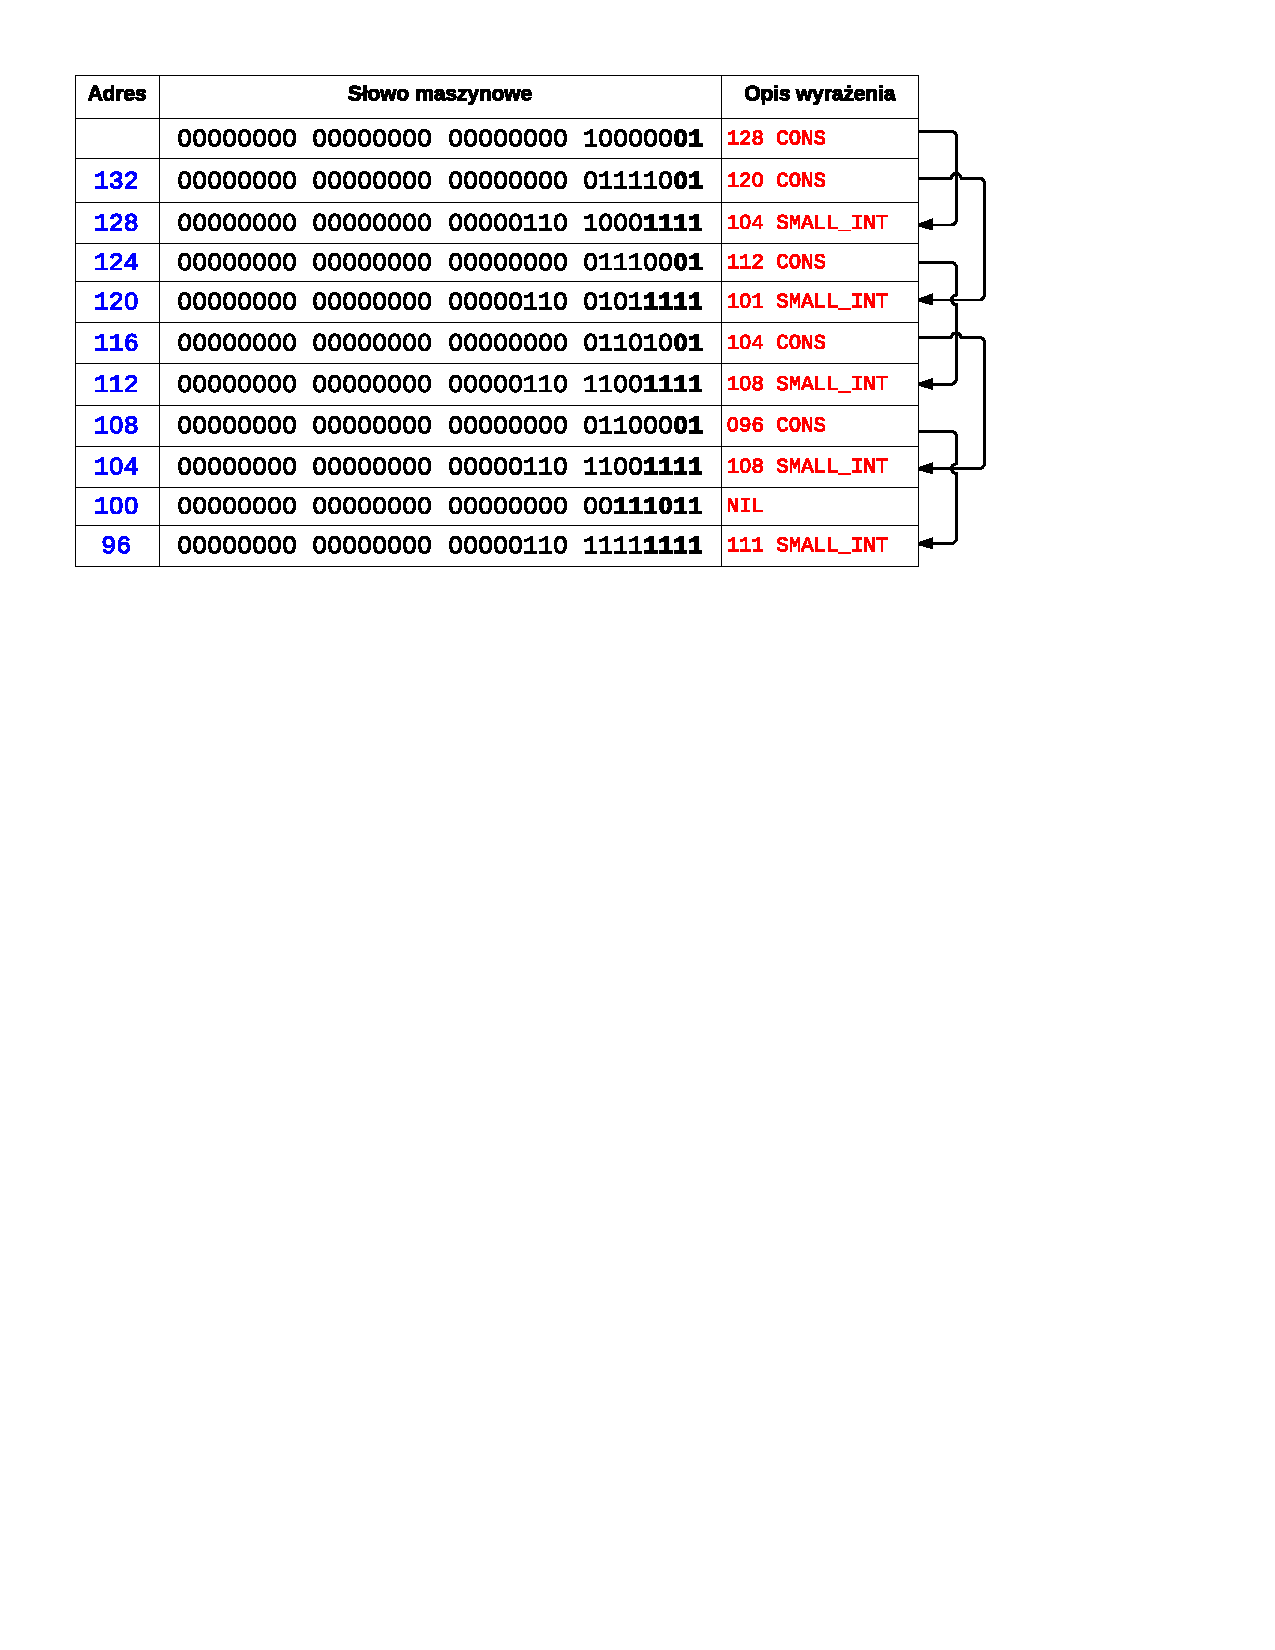
\includegraphics[scale=1, clip, trim=10mm 180mm 45mm 10mm]{list_on_heap}}
\caption{Przykład przechowywania listy na stercie procesu}
\label{fig:listonheap}
\end{figure}

Powyższy przykład dobrze ilustruje narzut pamięciowy jaki wprowadza sposób zapisu napisu przy użyciu listy. 
Informacja, która przy użyciu innych języków programowania może być zapisana przy użyciu 5 bajtów w języku Erlang potrzebuje aż 10 słów maszynowych (40 bajtów na architekturze 32-bitowej).
Receptą na tego typu problem, wprowadzoną w maszynie wirtualnej BEAM, jest binarny typ danych. Napis \texttt{"hello"} przy jego użyciu zajmowałby w pamięci 3 słowa maszynowe (nagłówek i~2~słowa przeznaczone na dane).
Typ ten jednak nie został zaimplementowany w obecnej wersji maszyny na system FreeRTOS.  

Jak można zauważyć zarówno złożoność obliczeniowa (czas dostępu do danych na liście jest liniowy) jak i pamięciowa przy wykorzystaniu tego typu danych jest dość znacząca.

\subsection{Krotki}
\label{sub:typyKrotki}

Kolejnym złożonym typem danym, z którego można korzystać w języku Erlang jest krotka, zajmująca spójny obszar pamięci. Z implementacyjnego punktu widzenia można porównać ją do tablicy zawierającej wyrażenia erlangowe.

Krotka jest jednym z typów opakowanych (\textbf{BOXED}), zatem referencja do niej z poziomu stosu procesu zawiera wskaźnik do nagłówka krotki. Nagłówek, podobnie jak pozostałe wyrażenia zajmuje jedno słowo maszynowe i przechowuje rozmiar krotki w postaci:
$$\texttt{AAAAAAAA AAAAAAAA AAAAAAAA AA\textbf{000000}}$$
gdzie bity \texttt{A} oznaczają rozmiar (arność) krotki. Wyrażenia wchodzące w skład krotki zajmują kolejne, następujące po nagłówku, słowa maszynowe.

Na rysunku \ref{fig:tupleonheap} zaprezentowany został przykład przechowywania danych wewnątrz krotki na stercie procesu, jak w przykładzie na rys. \ref{fig:listonheap}, czyli krotki \texttt{\{104,101,108,108,111\}}.

\begin{figure}[h]
\centerline{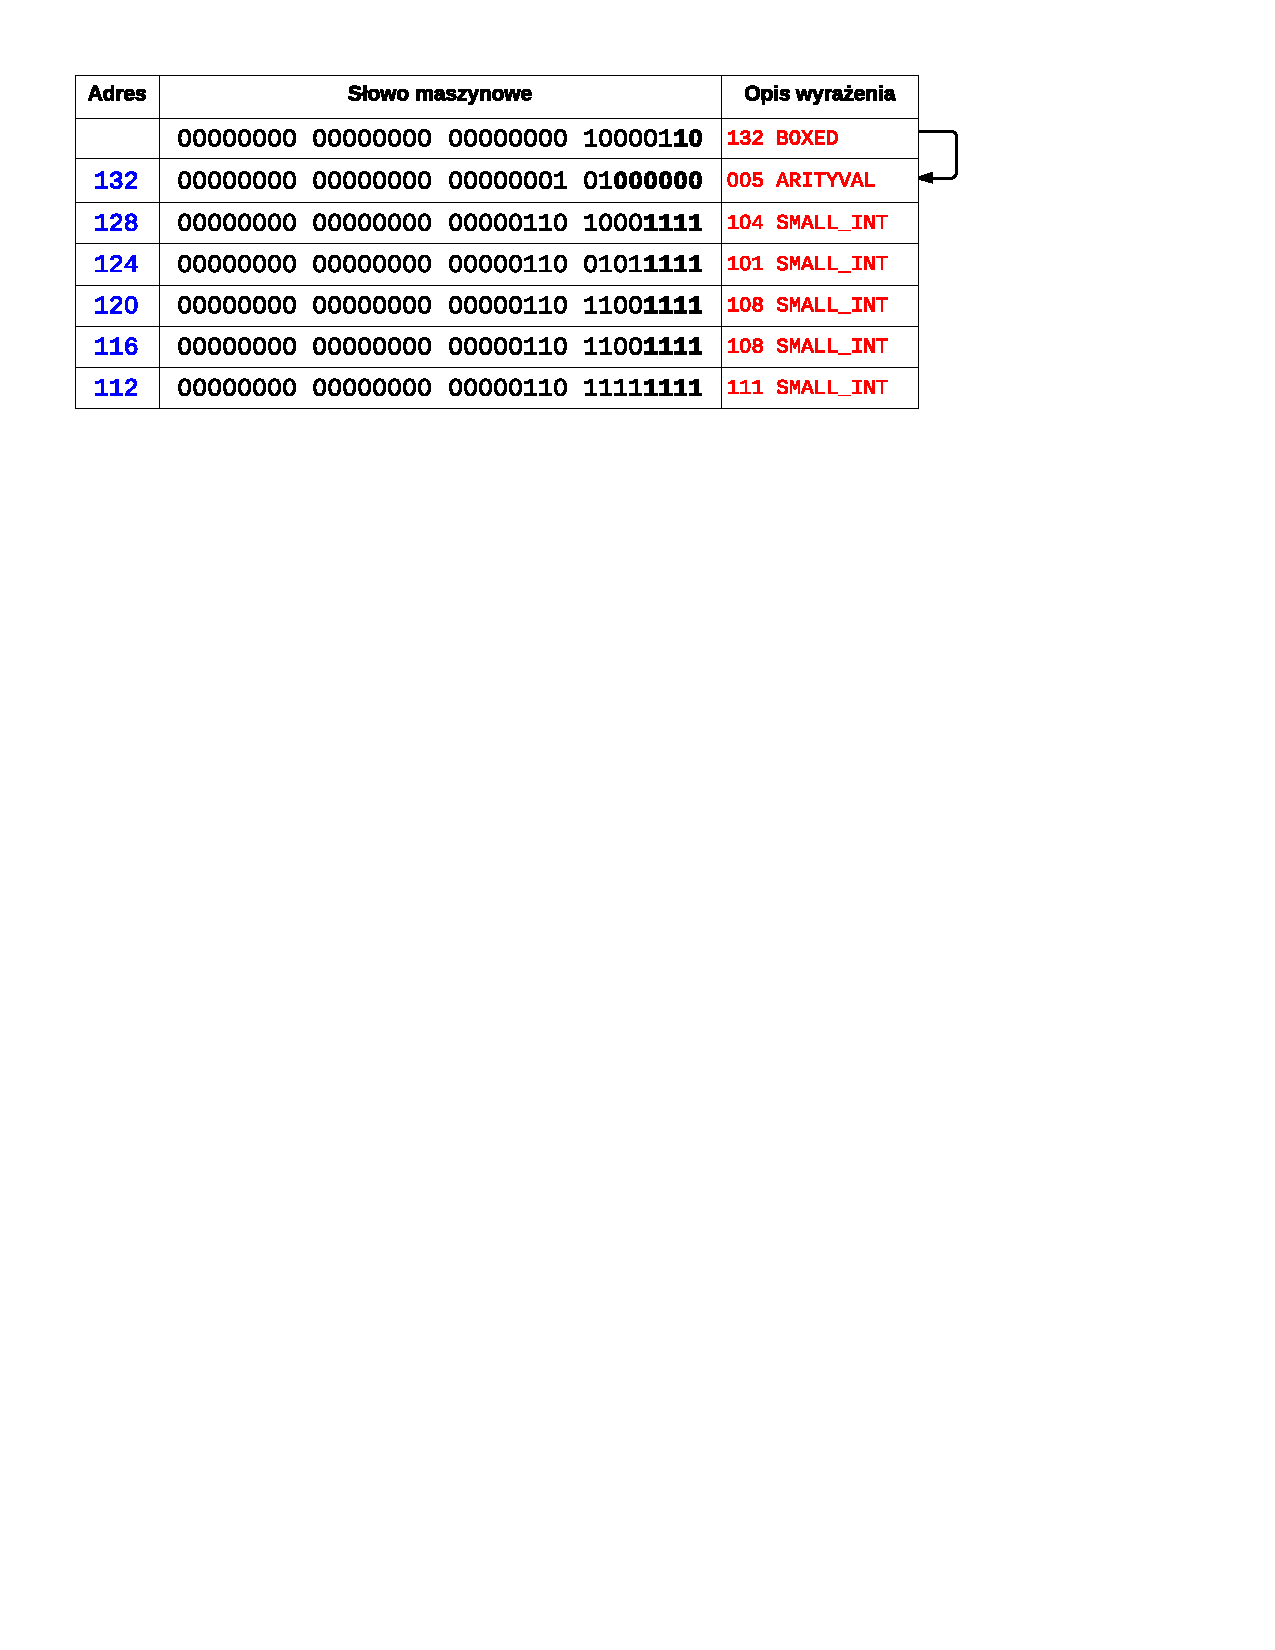
\includegraphics[scale=1, clip, trim=10mm 210mm 45mm 10mm]{tuple_on_heap}}
\caption{Przykład przechowywania krotki na stercie procesu}
\label{fig:tupleonheap}
\end{figure}

Ze względu na to, że krotka przechowuje dane w spójnym obszarze pamięci i dostęp do nich odbywa się w czasie stałym, użycie tego typu danych jest dobrym pomysłem w przypadku przechowywania danych tablicowych.

\subsection{Duże liczby}
\label{sub:typyBigs}

Drugim zaimplementowanym, opakowanym typem danych są duże liczby całkowite.
Wszystkie liczby całkowite, które nie mieszczą się w zakresie typu \textbf{SMALL\_INT}, czyli potrzebują do ich zapisania przynajmniej 29 bitów zapisywane są w typie danych \textbf{BIGNUM}.
Maszyna wirtualna zaimplementowana w ramach pracy, podobnie jak maszyna BEAM, implementuje własną arytmetykę implementującą operacje na tego typu liczbach.

Nagłówek typu \textbf{BOXED} ma w tym przypadku postać:
$$\texttt{AAAAAAAA AAAAAAAA AAAAAAAA AA\textbf{001S00}}$$
gdzie bity \texttt{A} oznaczają liczbę słów maszynowych, które składają się na całą liczbę bez znaku. Słowa te, w~kolejności od najmniej do najbardziej znaczącego, zajmują w pamięci kolejne słowa maszynowe po nagłówku. Bit \texttt{S} przechowuje znak liczby: \texttt{1} dla liczb ujemnych, {0} dla dodatnich.

Na rysunku \ref{fig:bignumonheap} zaprezentowany został przykład przechowania liczby $10^{28}$ na stercie procesu.

\begin{figure}[h]
\centerline{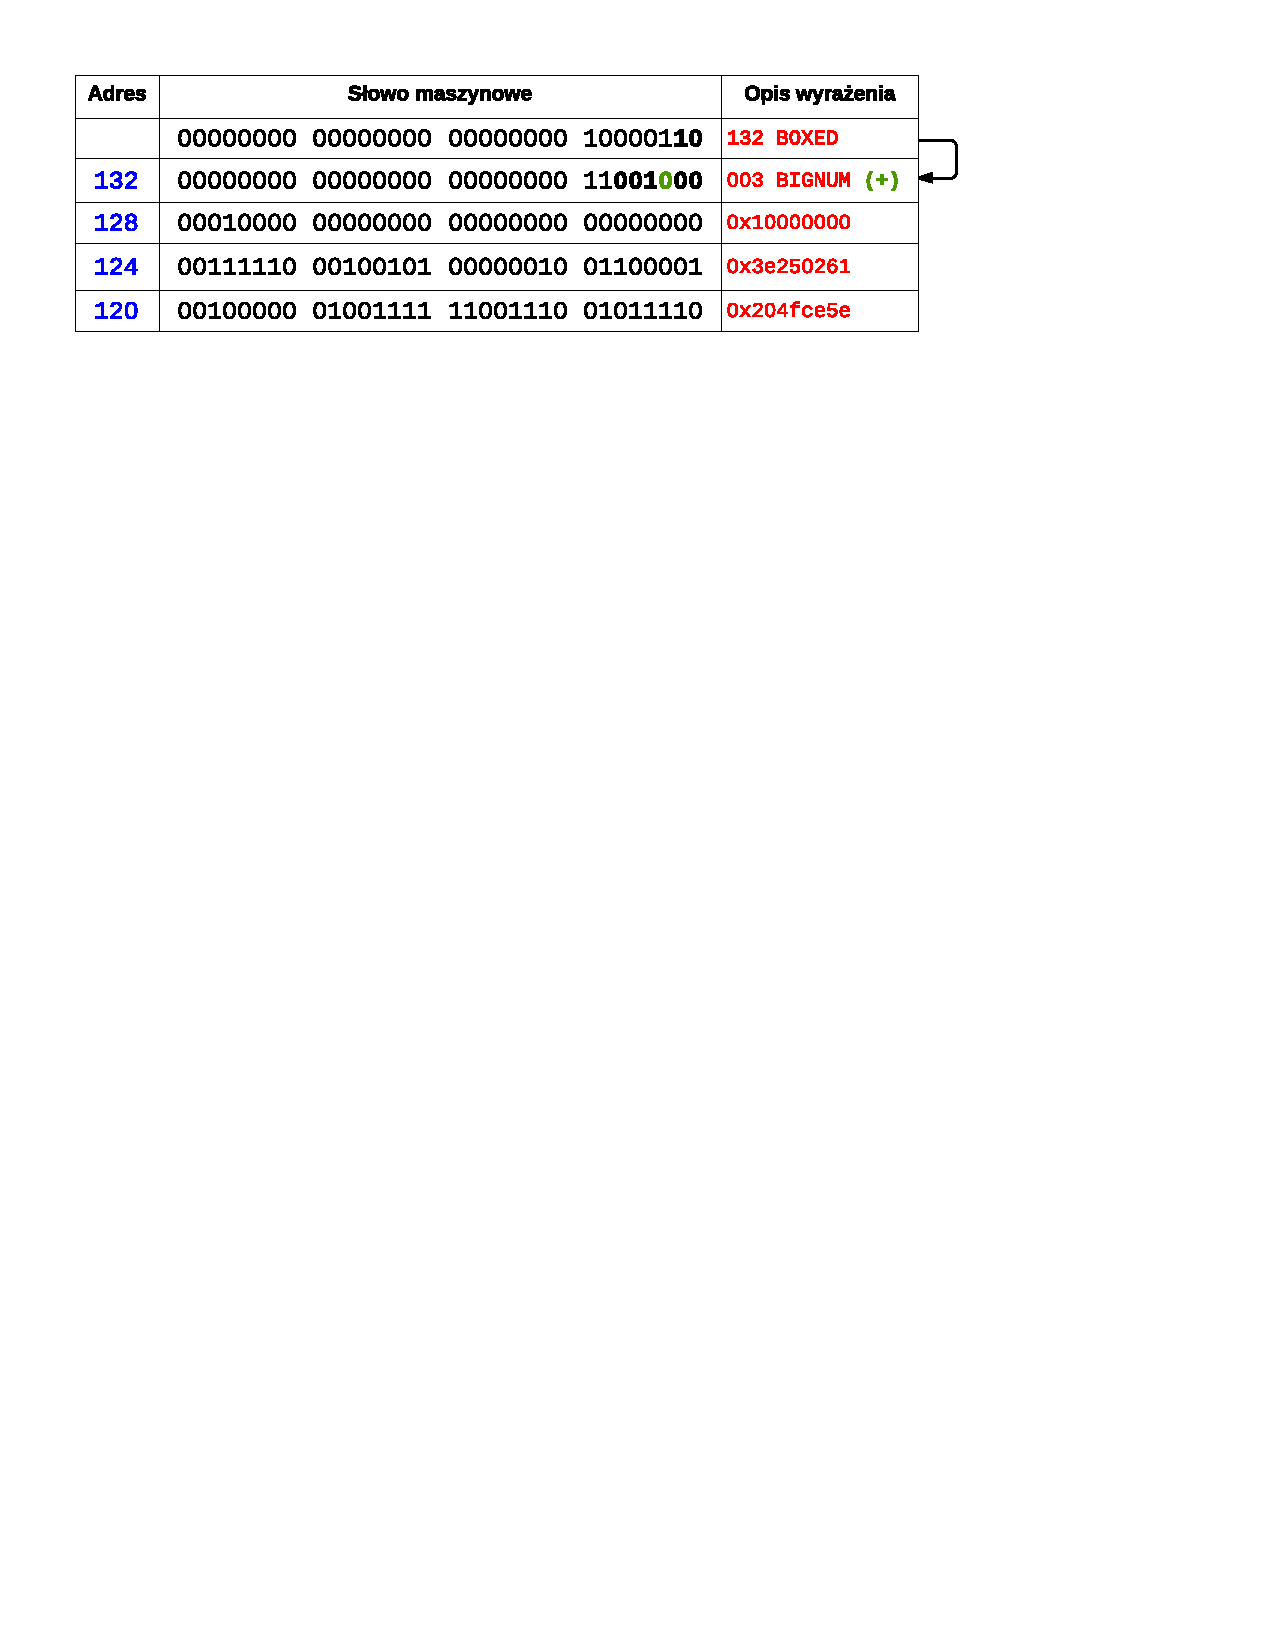
\includegraphics[scale=1, clip, trim=10mm 223mm 45mm 10mm]{bignum_on_heap}}
\caption{Przykład przechowywania dużej liczby na stercie procesu}
\label{fig:bignumonheap}
\end{figure}

\subsection{Lambdy}
\label{sub:typyLambda}

Typ danych wykorzystywany jest do identyfikacji obiektów funkcyjnych tworzonych dynamicznie w trakcie działania programu.
W maszynie wirtualnej BEAM obiekt taki może powstać w dwojaki sposób: przez wywołanie instrukcji \texttt{make\_fun2} lub funkcji wbudowanej \texttt{erlang:make\_fun/3}.
Bajty następujące po nagłówku typu danych zawierają informacje dotyczące miejsca początku kodu lambdy (każdemu obiektowi funkcyjnemu zdefiniowanemu w ramach danego modułu odpowiada osobna funkcja lokalna) a także wolnych zmiennych przez nią wykorzystywanych (czyli zmiennych, którym wartość przypisana została poza treścią lambdy, ale znajdujących się w jej kontekście).

Ten typ danych został w niniejszej maszynie wirtualnej zaimplementowany w ograniczonym zakresie, pozwalającym na definicję i wywołanie obiektów funkcyjnych w podstawowym zakresie.
Możliwe jest utworzenie lambdy poprzez jej zdefiniowanie, pod warunkiem że liczba jej wolnych zmiennych jest równa 0, lub na podstawie funkcji lokalnej (za pomocą konstrukcji \texttt{fun foo/2}).
Dodatkowo, utworzone lambdy nie podlegają odśmiecaniu przez algorytm \emph{garbage collectora}, dlatego też ich dynamiczne tworzenie w trakcie działania programu będzie prowadzić do wycieków pamięci.

Nagłówek typu danych ma następującą postać:
$$\texttt{00000000 00000000 00000000 00\textbf{000101}}$$

\subsection{Niezaimplementowane typy danych}
\label{sub:typyNiezaimplementowane}

Typy danych dostępne w maszynie BEAM, które nie zostały zaimplementowane w pracy to:
\begin{itemize}
\item \textbf{referencje} (tag \textbf{REF}) - referencje z~założenia używane są do oznaczania wiadomości wysyłanych do innych węzłów z uruchomioną maszyną wirtualną a klastrowanie nie jest wspierane przez implementowaną maszynę wirtualną;
\item \textbf{porty} (tag \textbf{PORT}) - porty używane są do identyfikacji procesów uruchomionych w systemie operacyjnym poza maszyną wirtualną Erlanga, a do których delegowane są pewne operacje, wykonywane na poziomie systemu operacyjnego. Wykonanie tych operacji (jak np. operacje na plikach) z~założenia może zająć pewien dłuższy okres czasu, co mogłoby zakłócić harmonogramowanie procesów. Typ danych nie został zaimplementowany, gdyż w maszynie wirtualnej wszystkie operacje wykonywane na poziomie mikrojądra zostały zaimplementowane przy pomocy funkcji wbudowanych (por. \ref{sec:maszynaBIF});
\item \textbf{liczby zmiennoprzecinkowe} (tag \textbf{FLONUM}) - ten typ danych również nie został zaimplementowany w~wersji maszyny opisywanej w pracy. Liczby zmiennoprzecinkowe rzadko wykorzystywane są w programowaniu urządzeń wbudowanych ze względu na bardzo duży narzut czasowych w przypadku mikrokontrolerów nie mających koprocesora (np. procesor ARM Cortex-M3 nie posiada FPU). M.in. z tego powodu do maszyny BEAM arytmetyka zmiennoprzecinkowa została dodana dopiero w wersji R8;
\item \textbf{binaria} (tagi \textbf{*\_BINARY}) - binarny typ danych włącznie ze wszystkimi operacjami dotyczącymi dopasowywania do nich zmiennych również nie został zaimplementowany w maszynie. Jest to funkcjonalność warta rozważenia w przypadku dalszej pracy nad maszyną ze względu na binarny charakter szeregowych interfejsów wejścia-wyjścia obsługiwanych przez mikrokontrolery. Podstawowe operacje na binariach do maszyny BEAM zostały dodane w wersji R7, bardziej zaawansowane były sukcesywnie dodawane od wersji R10;
\item \textbf{etykiety bloku \texttt{catch}} (tag \textbf{CATCH}) - typ danych służy do zapamiętywania na stosie procesu miejsc w kodzie, w których pojawiają się bloki \texttt{try} oraz \texttt{catch}. W przypadku błędu w programie, przed zakończeniem działania procesu, stos jest przeszukiwany w poszukiwaniu obecności ww. bloków. Instrukcje dotyczące łapania błędów nie zostały zaimplementowane w niniejszej maszynie wirtualnej.
\end{itemize}

%---------------------------------------------------------------------------
\section{Interpreter kodu maszynowego}
\label{sec:maszynaInterpreter}

Moduł opisany w niniejszym podrozdziale został zaimplementowany w pliku źródłowym \texttt{beam\_emu.c}.

\subsection{Maszyna stosowa a rejestrowa}
\label{sub:interpreterStosowa}

Spośród sposobów implementacji maszyny wirtualnej można wymienić dwa: maszynę stosową i~rejestrową.
Różnicę między tymi dwoma podejściami stanowi sposób przechowywania argumentów wywoływanej funkcji, miejsca zapisu wyniku jej wykonania oraz zmiennych tymczasowych przez nią używanych.

W przypadku maszyny stosowej dane te przechowywane są na stosie. Kolejne argumenty operacji umieszczane są na stosie za pomocą operacji \textbf{PUSH}, natomiast przed wykonaniem operacji zdejmowane są przez instrukcję \textbf{POP}. Instrukcje wykonywane przez maszynę wirtualną nie potrzebują zatem żadnych dodatkowych argumentów, gdyż te powinny być przed jej wywołaniem umieszczone na szczycie stosu, podobnie jak wynik zwrócony przez wykonaną instrukcję.

Z kolei w przypadku maszyny rejestrowej, powyższe informacje zapisywane są w zbiorze rejestrów.
Konsekwencją tego jest brak instrukcji manipulujących stosem w wykonywanym kodzie, co wpływa pozytywnie na szybkość działania interpretera kodu pośredniego.
Właściwe instrukcje wymagają jednak przekazania dodatkowych argumentów adresujących rejestry, w których znajdują się argumenty operacji i rejestr docelowy dla wyniku jej wykonania.
Efektem tego jest dłuższy zapis instrukcji w kodzie pośrednim niż w przypadku maszyny stosowej.
Dodatkowym atutem użycia rejestrów jest możliwość optymalizacji kodu polegającego na wyliczeniu i zapisaniu do rejestru pewnego pośredniego wyniku.
Wynik ten może następnie zostać wykorzystany przez kilka różnych instrukcji, zamiast wyliczania go od nowa przez każdą z nich.

Przykładami stosowych maszyn są maszyny języków takich jak Java czy .NET.
Z kolei przykładami maszyn rejestrowych są maszyny wirtualne języka Lua czy maszyna wirtualna Javy na system Android - Dalvik.

\subsection{Model interpretera}
\label{sub:interpreterModel}

Maszyna wirtualna języka Erlang (BEAM oraz maszyna zaimplementowana w pracy) jest również przykładem rejestrowej maszyny wirtualnej.

Interpreter korzysta z następujących rejestrów:
\begin{itemize}
\item rejestry \textbf{X\textsubscript{0}-X\textsubscript{255}} służące do przechowywania kolejnych argumentów z jakimi wywoływana jest funkcja, dodatkowo w rejestrze \textbf{X\textsubscript{0}} zapisywana jest wartość zwracana przez funkcję;
\item rejestry \textbf{Y} znajdujące się na stosie aktualnie uruchomionego procesu, służące do przechowywania zmiennych lokalnych;
\item rejestr \textbf{IP} przechowujący wskaźnik do aktualnie wykonywanej przez interpreter instrukcji;
\item rejestr \textbf{CP} przechowujacy adres powrotu - wskaźnik do instrukcji, którą interpreter powinien wykonać gdy nastąpi powrót z aktualnie wykonywanej funkcji.
\end{itemize}

Na listingu \ref{lis:maxS} zaprezentowany został przykładowy kod pośredni funkcji o arności 3, wyliczającej maksimum ze wszystkich jej argumentów, wykorzystujący do tego celu funkcję wbudowaną \texttt{erlang:max/2}. Wyjaśnienie działania poszczególnych operacji zostało zawarte w dodatku \ref{cha:operacjeBeam}.

\begin{lstlisting}[style=erlang, caption=Kod pośredni funkcji zwracającej maksimum z trzech argumentów, label=lis:maxS]
{allocate,1,3}.
{move,{x,2},{y,0}}.
{call_ext,2,{extfunc,erlang,max,2}}.
{move,{y,0},{x,1}}.
{call_ext_last,2,{extfunc,erlang,max,2},1}.
\end{lstlisting}

Na rysunkach od \ref{fig:max1} do \ref{fig:max8} zaprezentowano zawartość rejestrów X (interpretera) i Y (stos procesu) po wykonaniu poszczególnych operacji kodu powyższego dla argumentów: \texttt{5,7,9}. Zapis \texttt{\{l,1\}} oznacza, że wskaźnik do instrukcji wskazuje na linię 1 z przykładu na listingu \ref{lis:maxS}, z kolei \texttt{erlang:max/2} oznacza, że wskaźnik do instrukcji wskazuje na początek tej funkcji wbudowanej. Przez zapis \texttt{CP} rozumiana jest wartość wskaźnika \textbf{CP} w chwili wywołania funkcji. 

Jak można zauważyć na rys. \ref{fig:max1} wszystkie trzy argumenty zostały umieszczone w rejestrach \textbf{X}: 0,~1~i~2. Instrukcja \texttt{\{allocate,1,3\}}, znajdująca się w pierwszej linii powoduje rozszerzenie stosu procesu o 2 wyrażenia, z czego na szczycie stosu umieszczany jest adres powrotu, z jakim została wywołana funkcja, zapisany pod wskaźnikiem \textbf{CP}. Jeżeli w trakcie wykonania tej instrukcji konieczne byłoby uruchomienie \emph{garbage collectora}, drugi argument informuje o tym, że aktualnie w użyciu są 3 rejestry \textbf{X} i nie jest możliwe zwolnienie obszarów pamięci do których one się odnoszą.

W linii 2 (rys. \ref{fig:max3}) dokonane zostaje przeniesienie wyrażenia z rejestru \textbf{X\textsubscript{2}} do rejestru \textbf{Y\textsubscript{0}}, który jest pierwszym wyrażeniem na stosie poniżej jego szczytu.
Należy zauważyć, że pomimo wykorzystania stosu do zapisu zmiennych lokalnych, które nie zostaną zmodyfikowane pomiędzy wywołaniami funkcji, do operacji na nim nie wykorzystuje się operacji stosowych.
Nie należy zatem wiązać wykorzystania stosu procesu z faktem, że maszyna wirtualna jest maszyną stosową.

Przed wywołaniem funkcji \texttt{erlang:max/2} w linii 3, jako adres powrotu zostaje zapisana kolejna instrukcja w module, znajdująca się w linii 4. Argumentami wywoływanej funkcji są wartości znajdujące się w rejestrach \textbf{X\textsubscript{0}} i \textbf{X\textsubscript{1}}. Wywołana funkcja w momencie powrotu przepisuje wskaźnik powrotu (\textbf{CP}) na kolejną instrukcję do wykonania (\textbf{IP}). Wartość zwrócona z funkcji znajduje się w rejestrze \textbf{X\textsubscript{0}}. 

W linii 5 (rys. \ref{fig:max6}) wartość przechowywana na stosie zostaje przepisana do rejestru \textbf{X\textsubscript{1}}.
Drugie wywołanie funkcji \texttt{erlang:max/2} jest wywołaniem ogonowo-rekurencyjnym.
Dlatego też przykładowa funkcja odpowiedzialna jest za przywrócenie wskaźnika \textbf{CP} ze stosu i zwolnienie go jeszcze przed wywołaniem funkcji zewnętrznej. 
Wartość zwrócona z trójargumentowej funkcji znajduje się w rejestrze \textbf{X\textsubscript{0}}, a kolejna wykonana instrukcja będzie następująca po instrukcji, która ją wywołała.

\begin{figure}
\begin{multicols}{2}

\vspace{-4mm}
\begin{Figure}
 \centering
 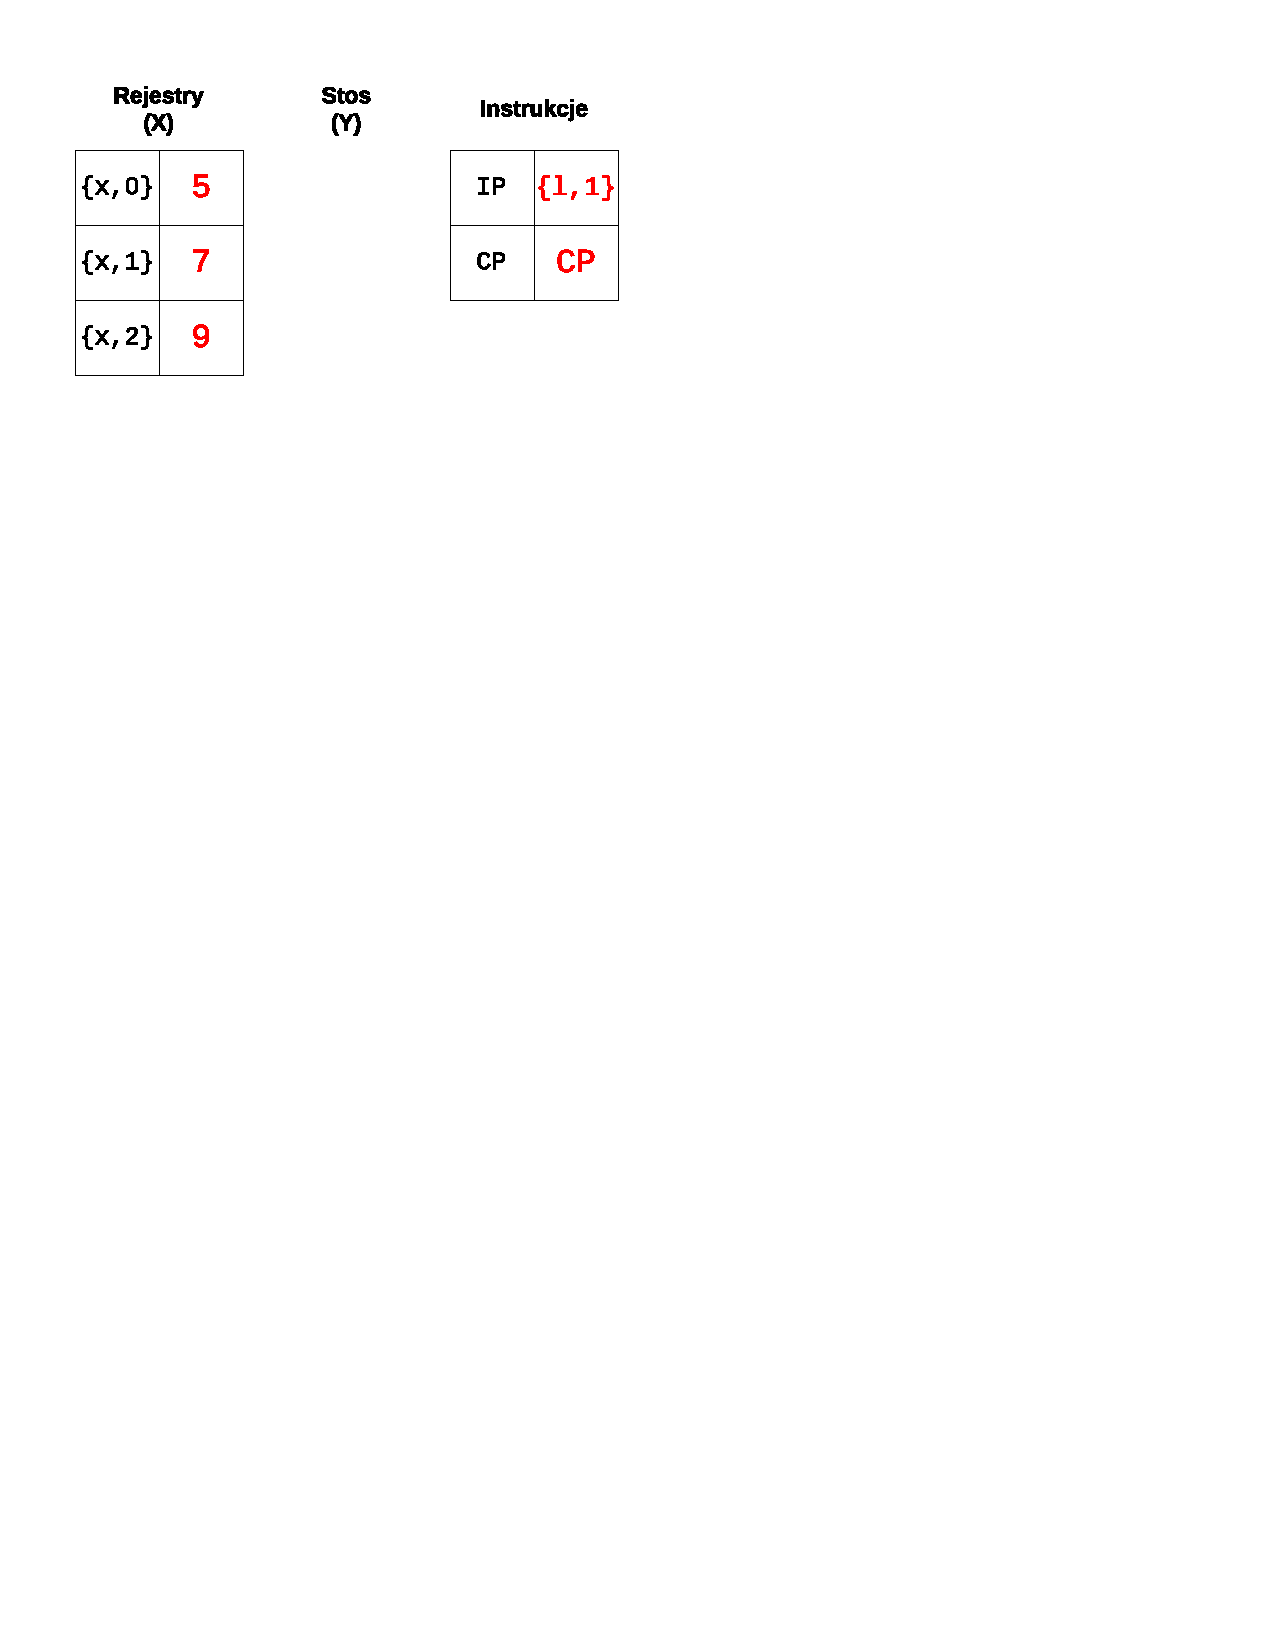
\includegraphics[scale=0.65, clip, trim=10mm 215mm 110mm 10mm]{interpreter_max_1}
\captionof{figure}{Rejestry przed wykonaniem instrukcji w linii 1}
\label{fig:max1}
\end{Figure}

\vspace{-4mm}
\begin{Figure}
 \centering
 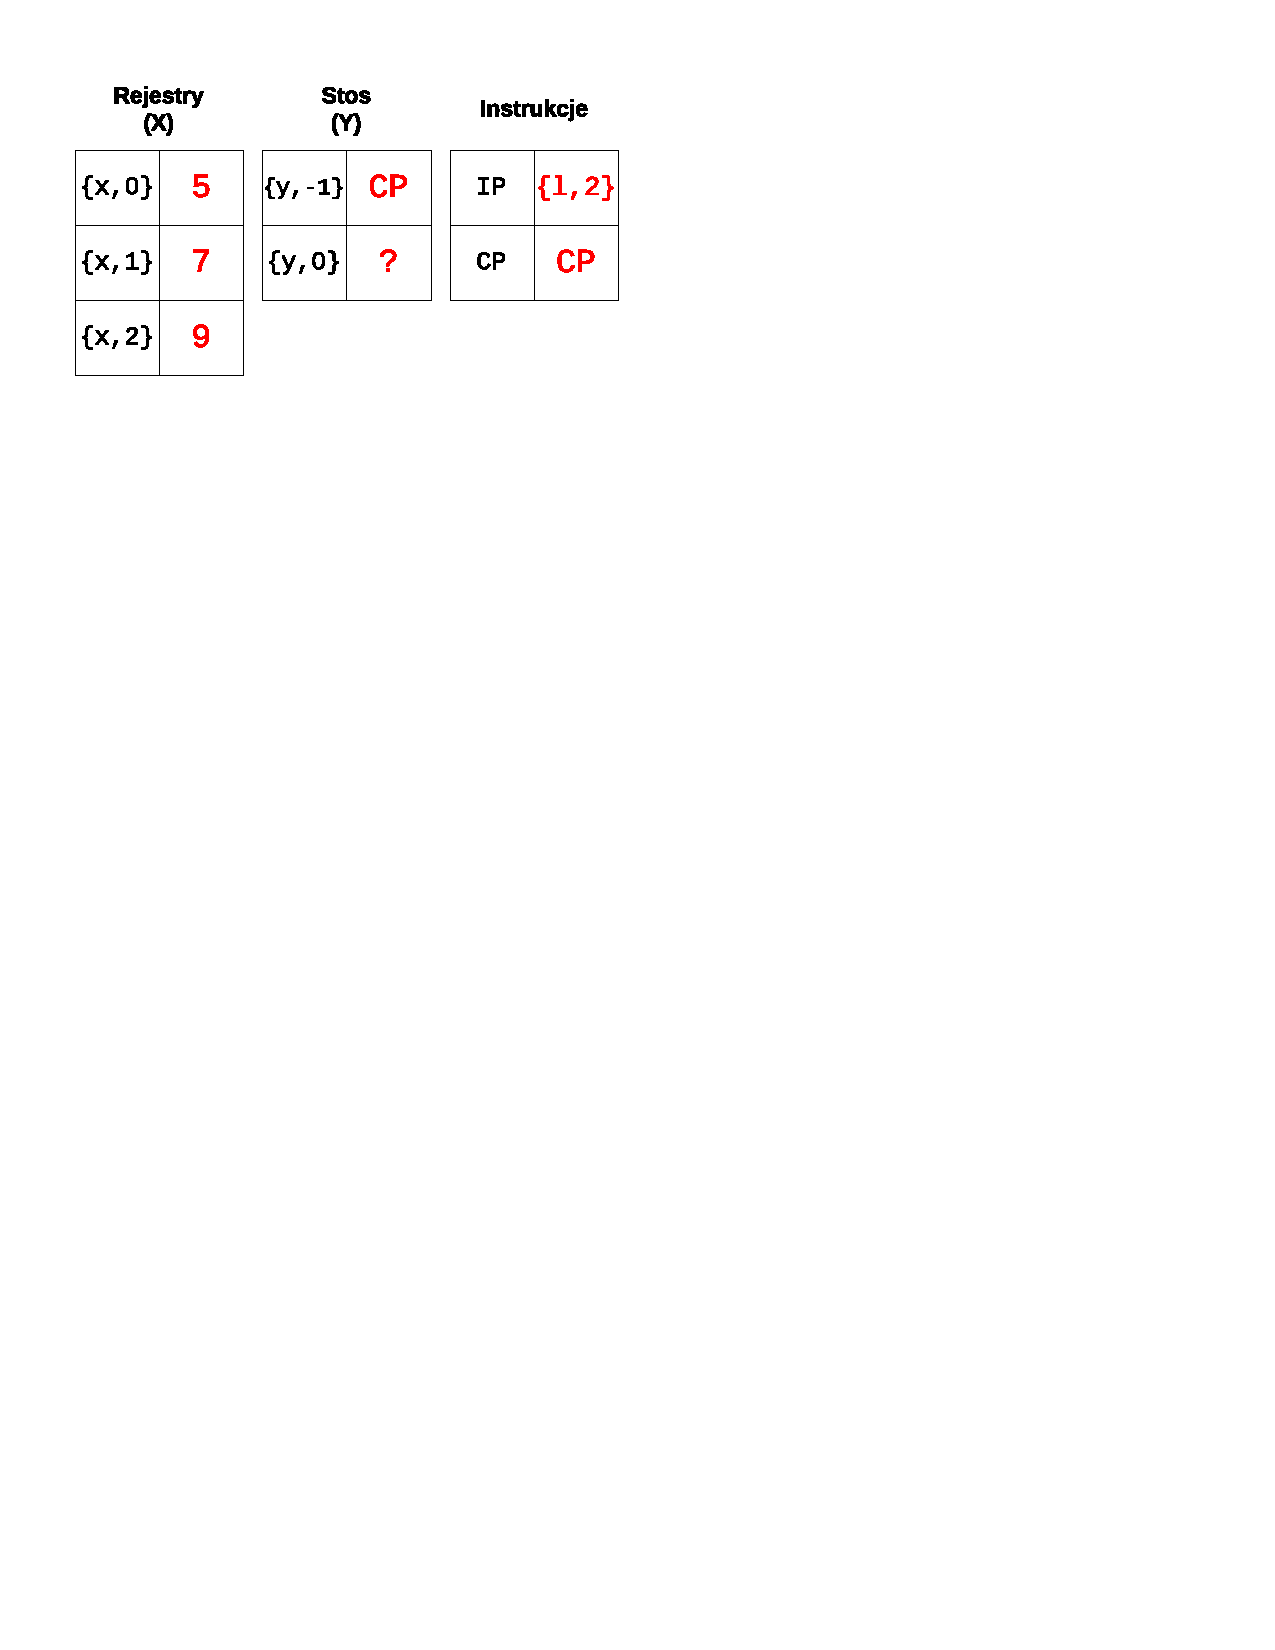
\includegraphics[scale=0.65, clip, trim=10mm 215mm 110mm 10mm]{interpreter_max_2}
\captionof{figure}{Rejestry przed wykonaniem instrukcji w linii 2}
\label{fig:max2}
\end{Figure}

\vspace{-4mm}
\begin{Figure}
 \centering
 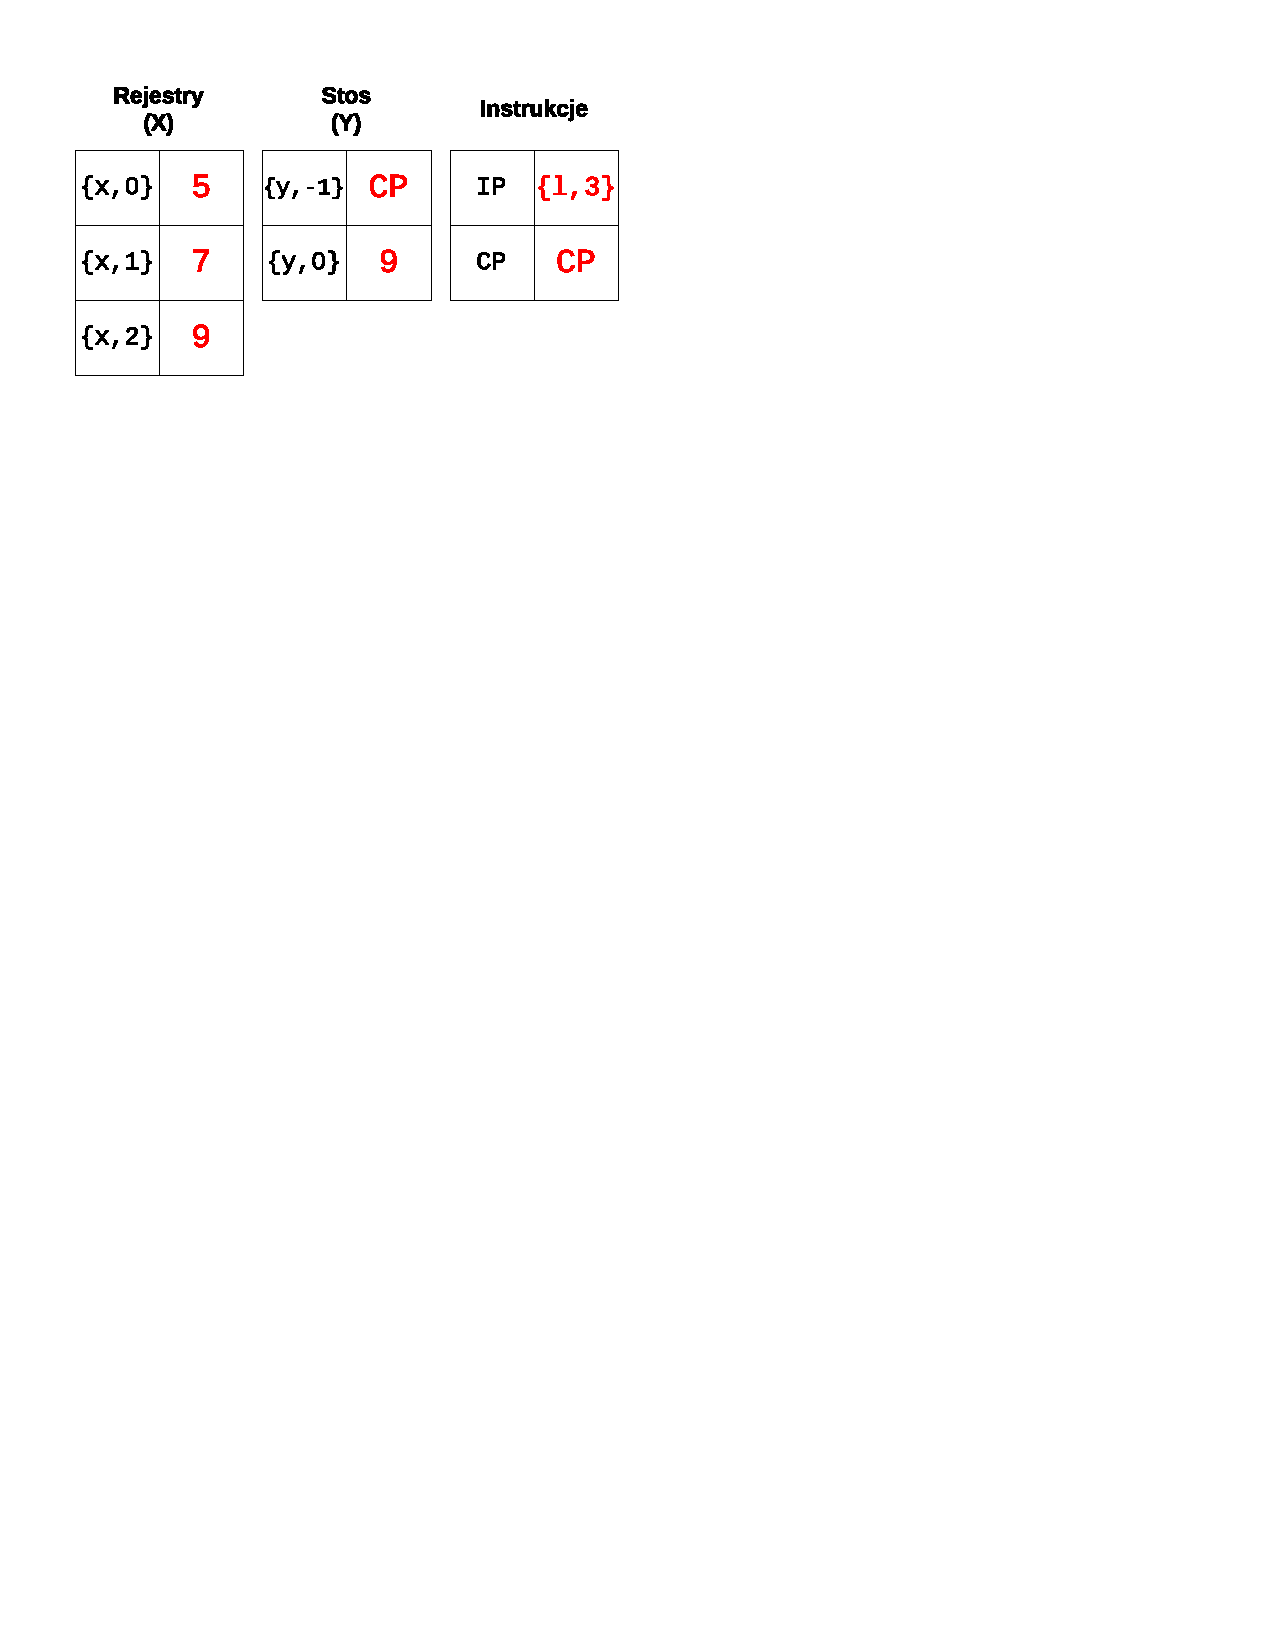
\includegraphics[scale=0.65, clip, trim=10mm 215mm 110mm 10mm]{interpreter_max_3}
\captionof{figure}{Rejestry przed wykonaniem instrukcji w linii 3}
\label{fig:max3}
\end{Figure}

\vspace{-4mm}
\begin{Figure}
 \centering
 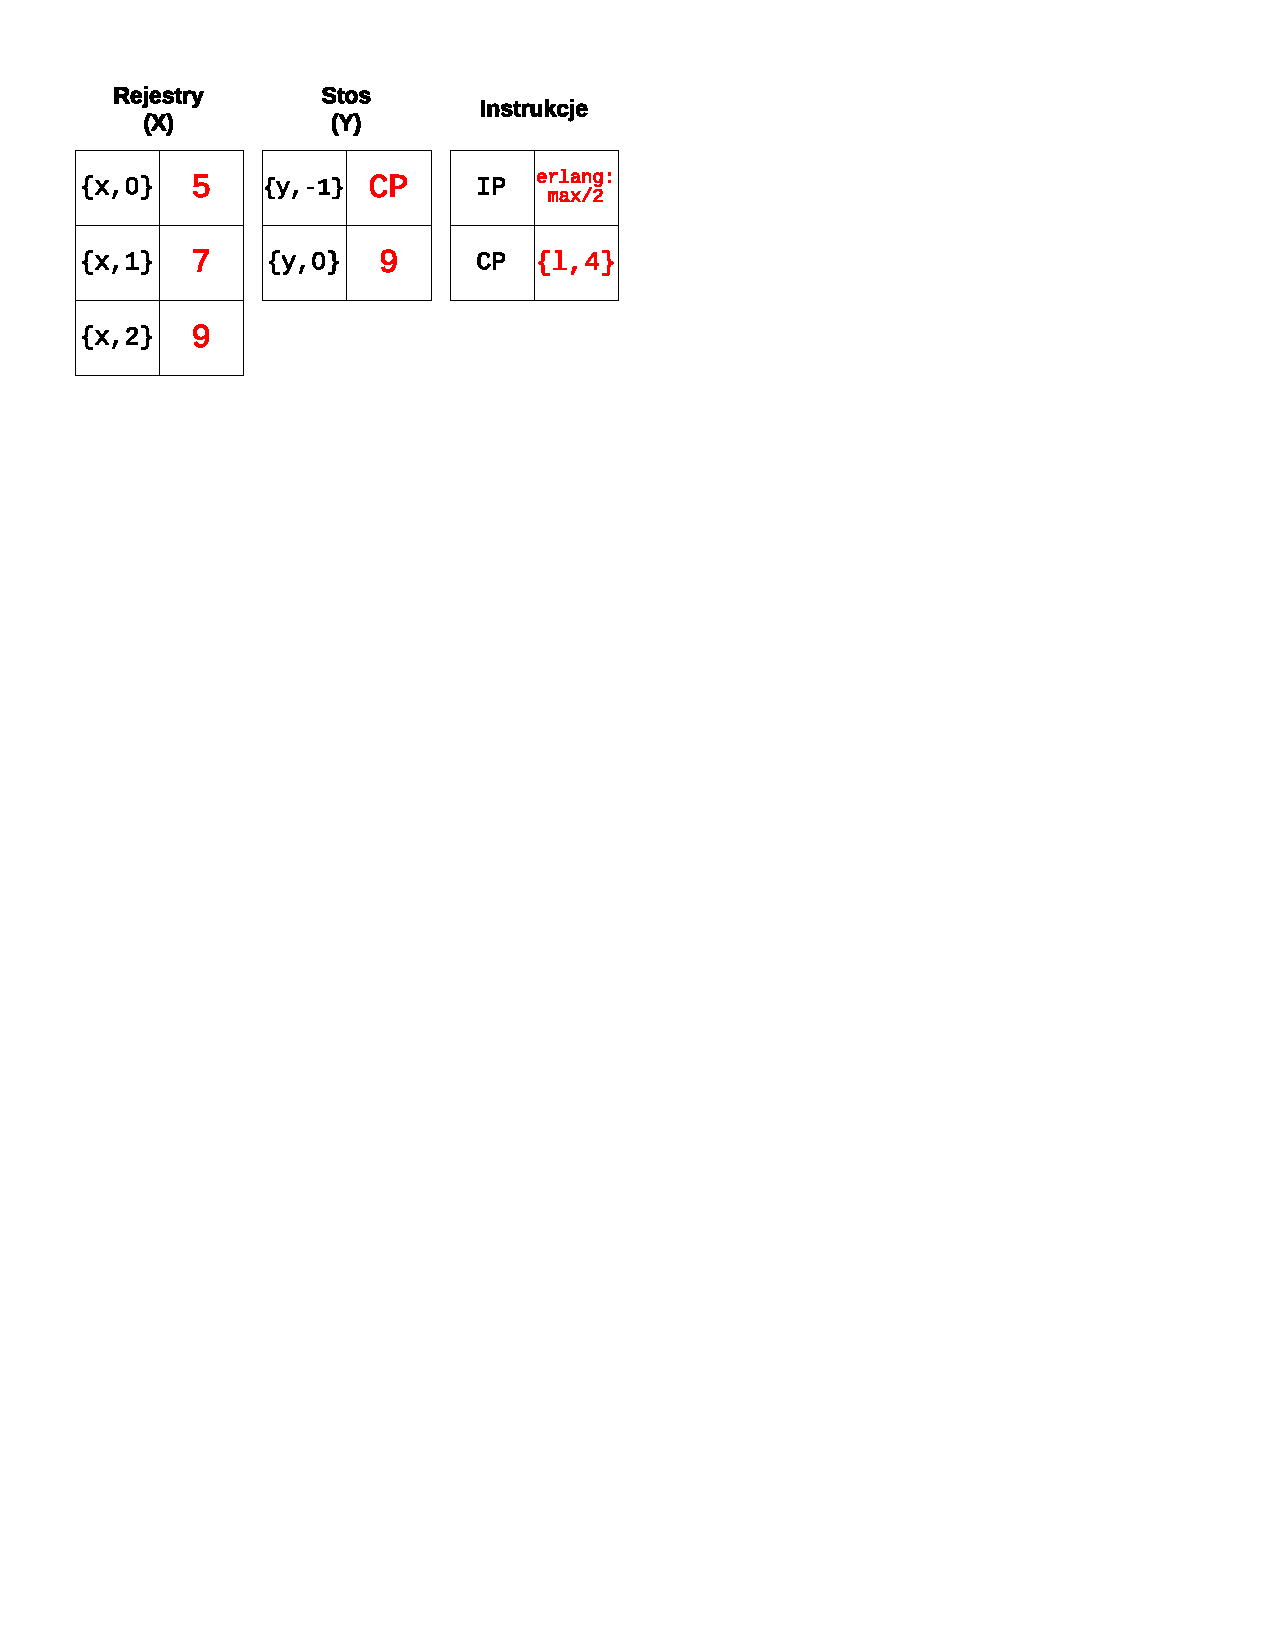
\includegraphics[scale=0.65, clip, trim=10mm 215mm 110mm 10mm]{interpreter_max_4}
\captionof{figure}{Rejestry przed wywołaniem funkcji w linii 3}
\label{fig:max4}
\end{Figure}

\vspace{-4mm}
\begin{Figure}
 \centering
 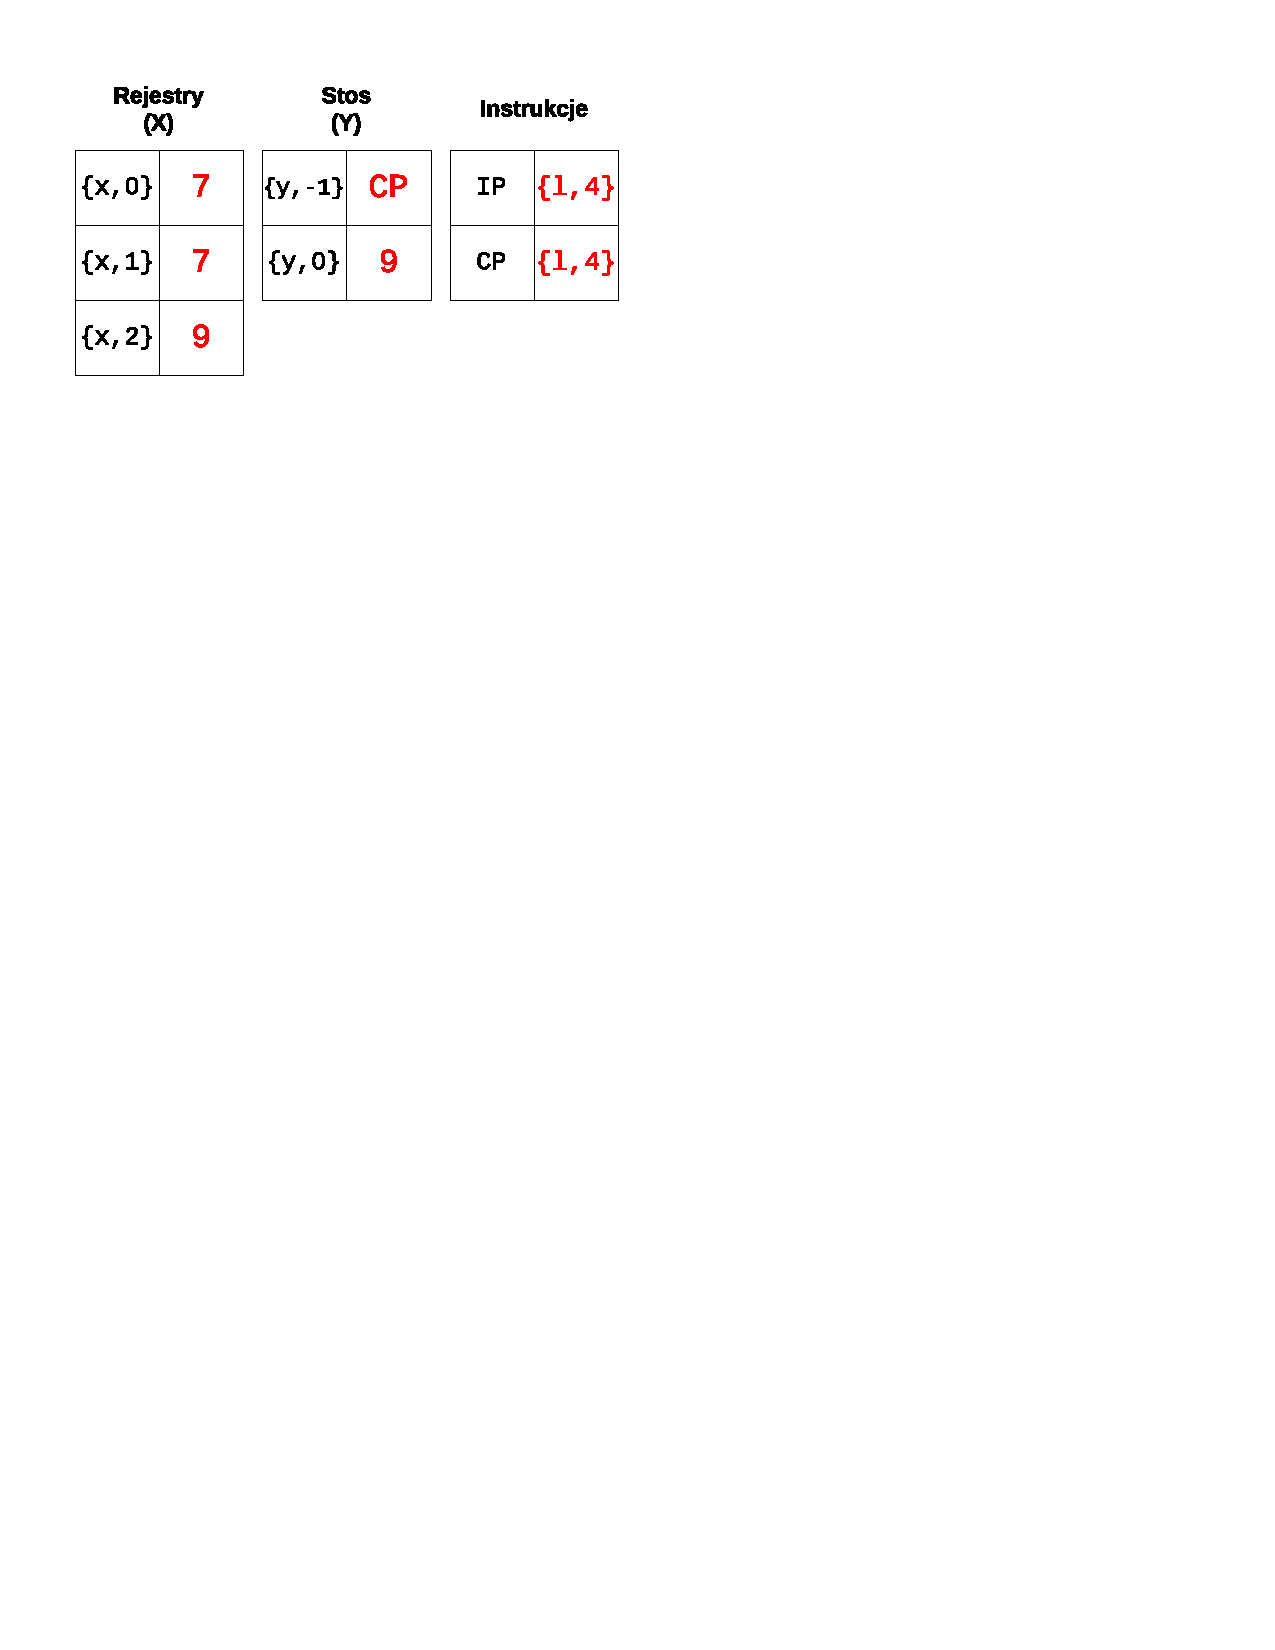
\includegraphics[scale=0.65, clip, trim=10mm 215mm 110mm 10mm]{interpreter_max_5}
\captionof{figure}{Rejestry przed wykonaniem instrukcji w linii 4}
\label{fig:max5}
\end{Figure}

\vspace{-4mm}
\begin{Figure}
 \centering
 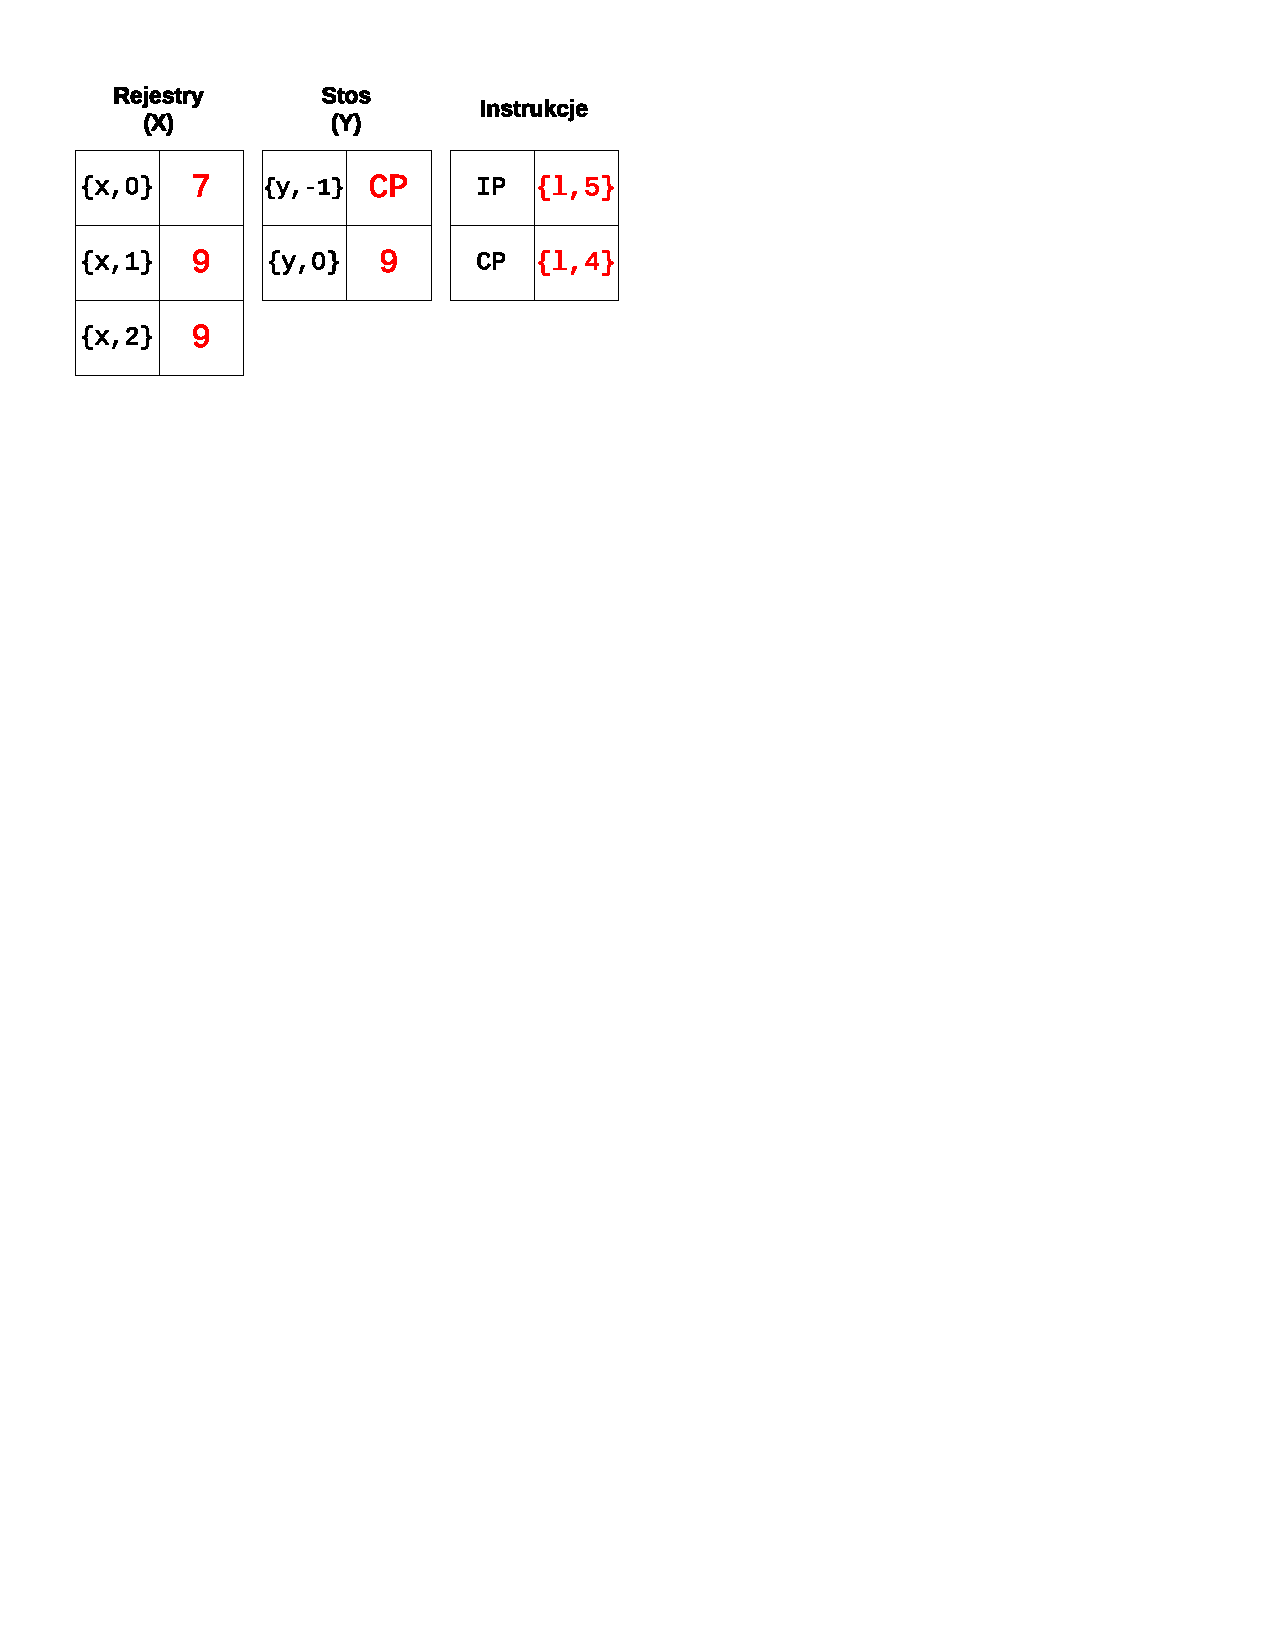
\includegraphics[scale=0.65, clip, trim=10mm 215mm 110mm 10mm]{interpreter_max_6}
\captionof{figure}{Rejestry przed wykonaniem instrukcji w linii 5}
\label{fig:max6}
\end{Figure}

\vspace{-4mm}
\begin{Figure}
 \centering
 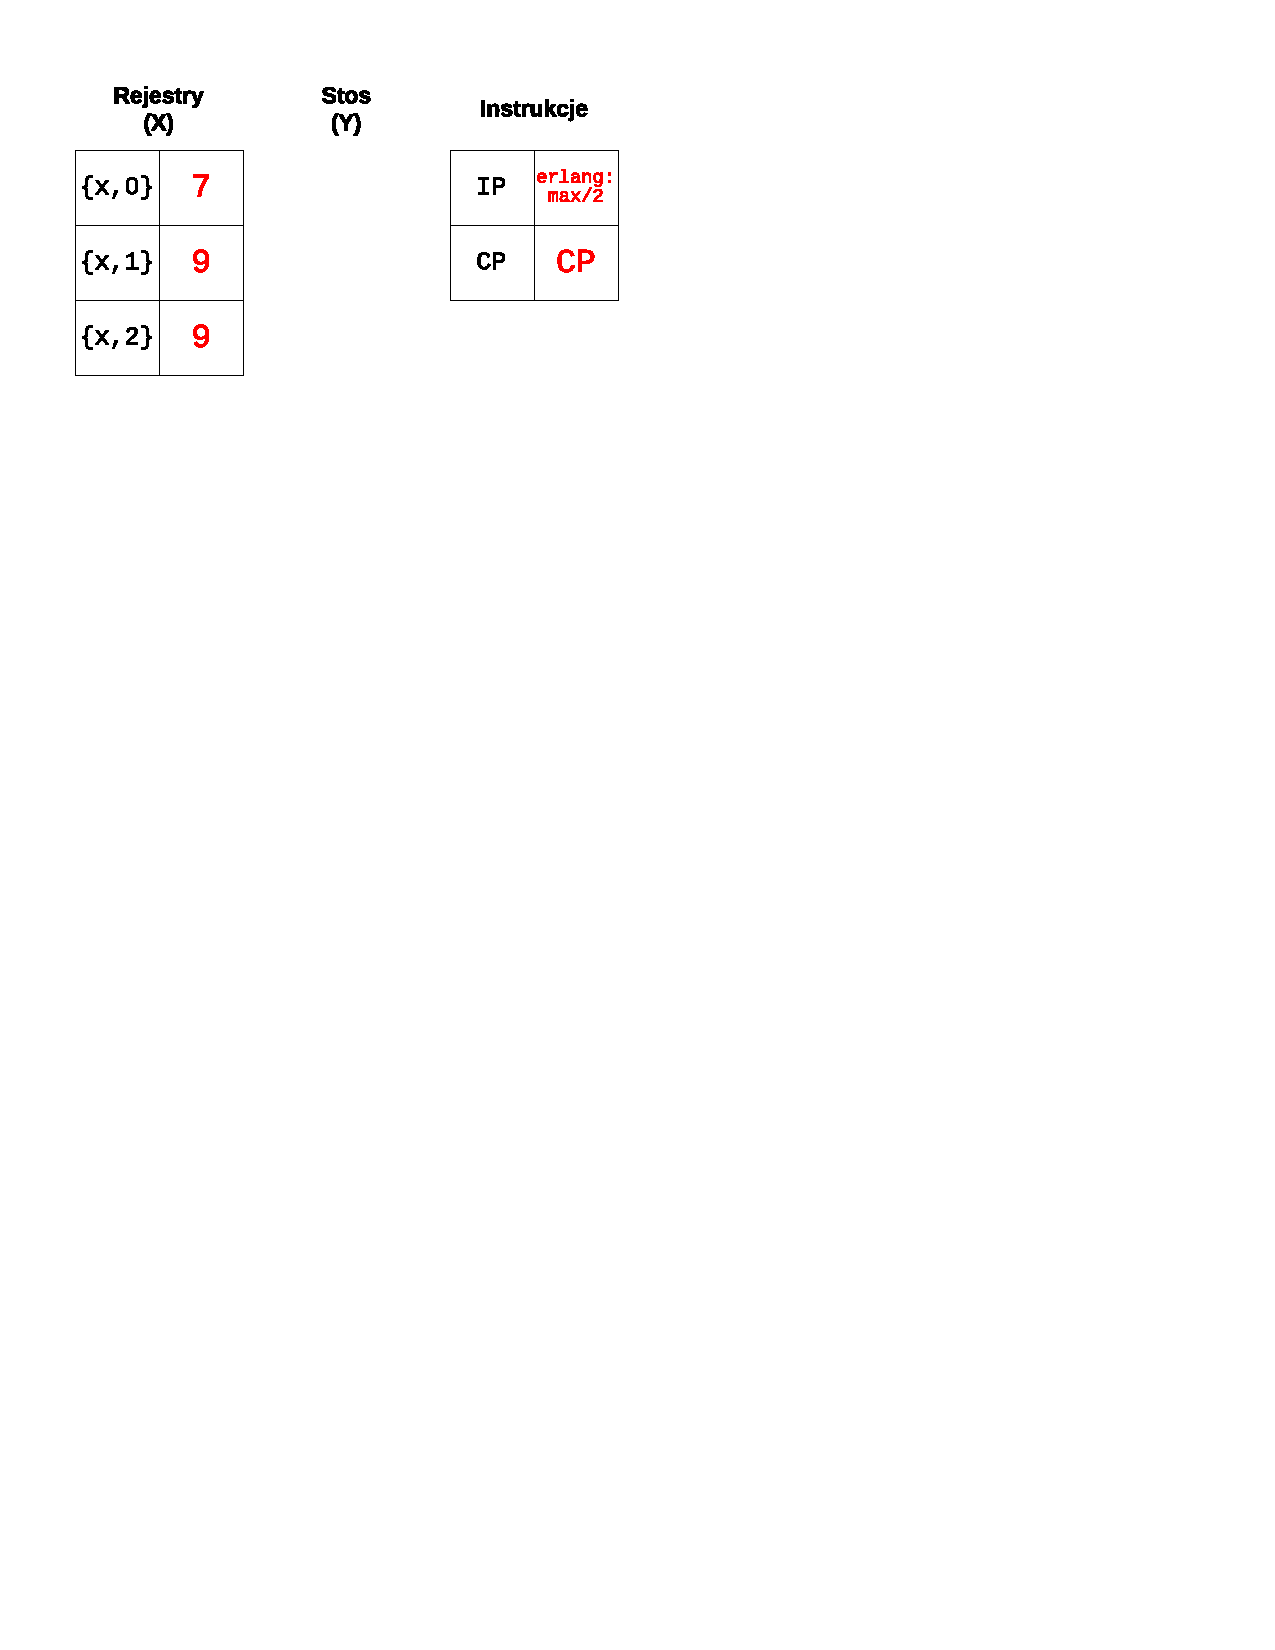
\includegraphics[scale=0.65, clip, trim=10mm 215mm 110mm 10mm]{interpreter_max_7}
\captionof{figure}{Rejestry przed wywołaniem funkcji w linii 5}
\label{fig:max7}
\end{Figure}

\vspace{-4mm}
\begin{Figure}
 \centering
 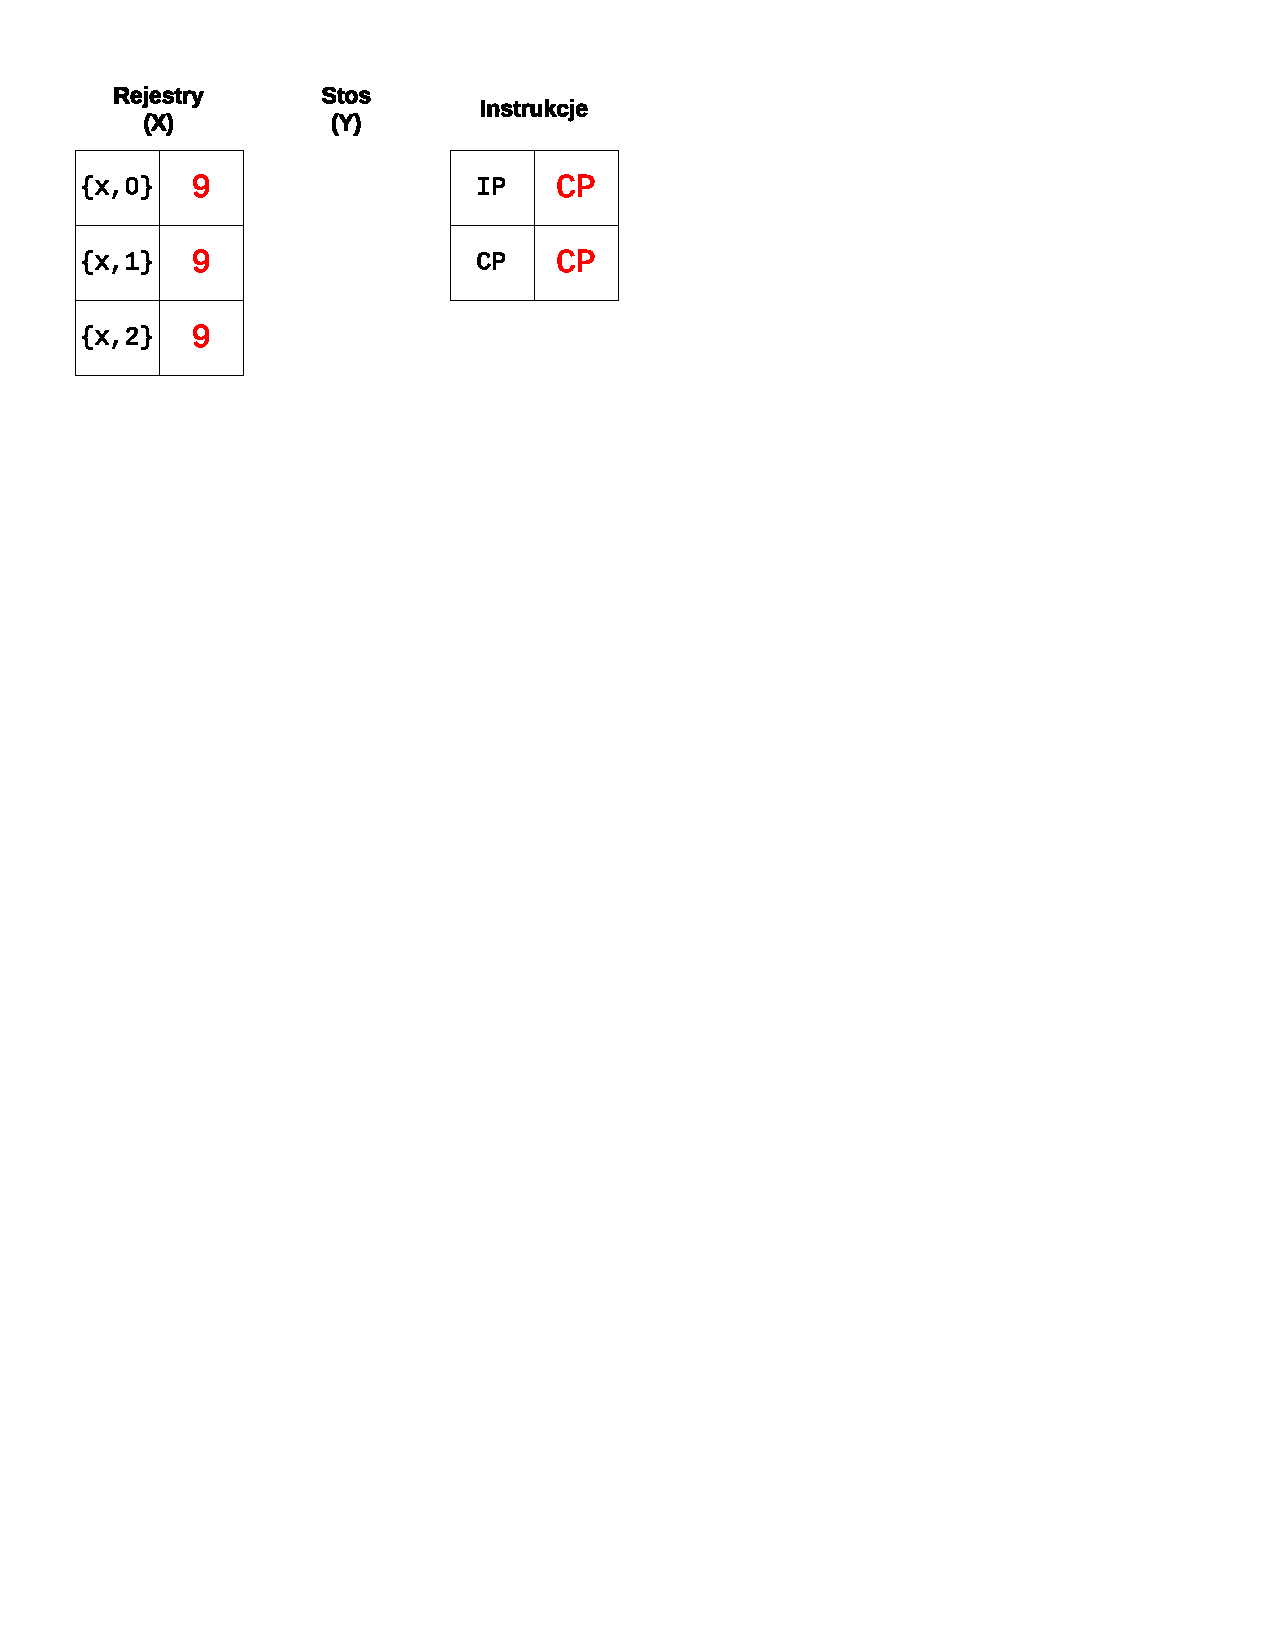
\includegraphics[scale=0.65, clip, trim=10mm 215mm 110mm 10mm]{interpreter_max_8}
\captionof{figure}{Rejestry po wykonaniu instrukcji w~linii 5, a zarazem i całej funkcji}
\label{fig:max8}
\end{Figure}
\end{multicols}
\end{figure}

\subsection{Sposób implementacji}
\label{sub:interpreterImplementacja}

Z implementacyjnego punktu widzenia kod interpretera kodu pośredniego w maszynie zaimplementowanej w pracy interpretuje kod adresowany bezpośrednio (\emph{Directly Threaded Code} \cite{Ertl}). Oznacza to, że operacja przekazywana do interpretera zapisana jest nie w postaci opkodu, ale zawiera wskaźnik do etykiety implementującej daną instrukcję. Odpowiedniej podmiany, w momencie ładowania pliku z modułem dokonuje \emph{loader}.

Maszyna wirtualna BEAM implementuje także sposób adresowania operacji przez ich opkod, na wypadek gdyby kompilator języka C użyty do jej kompilacji nie obsługiwał rozszerzenia standardu GNU C,~jakim są wskaźniki do etykiet.
Metoda \emph{Switch Threading} nie wymaga podmiany w żaden sposób oryginalnych opkodów, jednak interpretacja kodu pośredniego z jej użyciem jest dużo wolniejsza.
Powodem tego jest fakt, że kod każdej operacji przed jej wykonaniem należy sprawdzić z całym zestawem obsługiwanych opkodów w instrukcji \texttt{switch}, aż do napotkania właściwej.
W maszynie na system FreeRTOS wykorzystano oba sposoby adresowania operacji, a używany może zostać wybrany na poziomie konfiguracji maszyny wirtualnej (por. \ref{cha:config}).

Zestaw instrukcji zaimplementowanych w maszynie wirtualnej wraz z opisem ich działania został zaprezentowany w dodatku \ref{cha:operacjeBeam}.
Dodatek ten wymienia operacje, jakie możliwe są do otrzymania w pliku z kodem pośrednim z kompilatora języka Erlang.
Maszyna wirtualna BEAM implementuje jednak nieco większy zestaw instrukcji, który zostaje podmieniany w kodzie maszynowym w momencie ładowania modułu do pamięci (por. \ref{sec:maszynaLoader}).

Dodatkowymi operacjami, wykorzystywanymi wewnętrznie przez maszynę wirtualną, zaimplementowanymi w interpreterze są: \texttt{beam\_apply/0} oraz \texttt{normal\_exit/0}, służące do kontroli cyklu życia procesu.
W momencie startu procesu jako pierwsza instrukcja do wykonania (wskaźnik \textbf{IP}) zostaje ustawiona pierwsza z tych operacji, po wcześniejszym zapisaniu do pierwszych trzech rejestrów \textbf{X}: modułu, funkcji i listy argumentów będących początkowymi dla tego procesu.
Następnie operacja ta wywołuje właśnie tę funkcję.
Jako adres powrotu z wywołania funkcji początkowej (wskaźnik \textbf{CP}) ustawiana jest druga z dodatkowych instrukcji, która kończy działanie procesu z powodu osiągnięcia końca jego kodu.

%---------------------------------------------------------------------------
\section{Procesy}
\label{sec:maszynaProcesy}

Logika procesu opisana w niniejszym podrozdziale została zaimplementowana w pliku źródłowym \texttt{erl\_process.c}.

\subsection{Tablica procesów}
\label{sub:procTablica}

Stuktura procesów przechowywana jest w prealokowanej tablicy o konfigurowalnym rozmiarze.
W~zaimplementowanej maszynie domyślnie rozmiar ten wynosi 25.
Tak mała liczba procesów została wybrana ze względu na duże ograniczenia zasobów platformy docelowej dla maszyny.

Procesy identyfikowane są wewnątrz maszyny wirtualnej przez identyfikator procesu (\textbf{PID}, por. \ref{sub:typyImmediates}).
Ten bezpośredni typ danych przechowuje indeks procesu w ww. tablicy, dzięki czemu możliwe jest szybkie znalezienie struktury procesu, który konieczny jest do wykonania instrukcji przez interpreter kodu.

\subsection{Struktura procesu}
\label{sub:procStruktura}

W strukturze przechowującej informacje o procesie zostały zawarte dane niezbędne do poprawnego wykonywania przez niego kodu.
Spośród nich można wymienić:
\begin{itemize}
\item wspomniany wcześniej identyfikator procesu (\textbf{PID});
\item blok pamięci zajmowany przez wyrażenia wykorzystywane przez proces, zawierający stertę i stos. Został on szczegółowo opisany w podrozdziale \ref{sec:maszynaGC};
\item wskaźniki przechowujące aktualnie wykonywaną przez proces instrukcję oraz adres powrotu;
\item liczba redukcji jakie pozostały do wywłaszczenia procesu;
\item uchwyt do zadania w systemie FreeRTOS, w kontekście którego wykonywany jest kod procesu;
\item pamięć do przechowania wartości rejestrów \textbf{X} w sytuacji gdy proces przestanie być wykonywany na rzecz innego procesu (por. \ref{sec:maszynaScheduler});
\item kolejka wiadomości, które zostały wysłane do procesu;
\item lista procesów połączonych z danym procesem poprzez \emph{link} (por. \ref{sec:maszynaBledy});
\item flagi procesu, ustawiane przez funkcję \texttt{erlang:process\_flag/2};
\item informacje statystyczne związane z cyklem życia procesu, takie jak liczba wykonanych redukcji czy liczba wykonanych odśmieceń na procesie w trakcie jego działania.
\end{itemize}

Podstawową różnicą między implementacją maszyny a maszyny BEAM jest sposób wykonywania kodu pośredniego procesu.
Maszyna BEAM implementuje własny algorytm harmonogramowania, biorąc na siebie odpowiedzialność za utrzymywanie kolejki procesów do wykonania i zarządzania kolejnością ich wykonania. Logika procesu nie jest zatem opakowana w żadną warstwę abstrakcji. 
Z kolei maszyna zaimplementowana w pracy do zarządzania kolejnością procesów wykorzystuje \emph{scheduler} wbudowany w mikrojądro FreeRTOS, a procesy są instancjami zadań przez niego zarządzanych (por. podrozdział \ref{sec:rtosScheduler}).
Powodem wykorzystania takiego podejścia jest mały narzut pamięciowy i czasowy związany z uruchamianiem zadań, a także wbudowana obsługa priorytetów zadań i możliwość konfiguracji parametrów planisty.

Różnicą w strukturze procesu jest także uproszczenie obszaru pamięci dla wyrażeń procesu do jednej, podstawowej sterty. 
Maszyna BEAM wykorzystuje bardziej zaawansowane, generacyjne podejście przechowując wyrażenia na dwóch stertach.
Technika ta opisana została w podrozdziale \ref{sec:maszynaGC}.

W maszynie rozważanej w pracy nie została także zaimplementowany słownik procesu.

\subsection{Komunikacja międzyprocesowa}
\label{sub:procKolejka}

Komunikacja między procesami w maszynie wirtualnej jest zapewniona dzięki instrukcjom:
\begin{itemize}
\item \texttt{send}, służącej do wysłania wiadomości do innego procesu;
\item \texttt{wait} i \texttt{wait\_timeout} zawieszających działanie procesu aż do momentu otrzymania wiadomości lub przeterminowania;
\item \texttt{loop\_rec}, \texttt{remove\_message} i \texttt{loop\_rec\_end}, wykonujących operacje na kolejce wiadomości.
\end{itemize}

Mechanizm wysyłania wiadomości do procesu został zaprezentowany na rysunkach od \ref{fig:mp1} do \ref{fig:mp4}.

Na początku (rys. \ref{fig:mp1}) w kolejce wiadomości procesu odbierającego znajduje się jedna wiadomość (\textbf{M\textsubscript{0}}).
Wskaźnik aktualnej wiadomości ustawiony jest na pierwszą wiadomość w kolejce, oznaczoną kolorem czerwonym.
Zostanie on wykorzystany przez proces w momencie osiągnięcia przez kod procesu bloku \texttt{receive}.

\begin{figure}[h]
\centerline{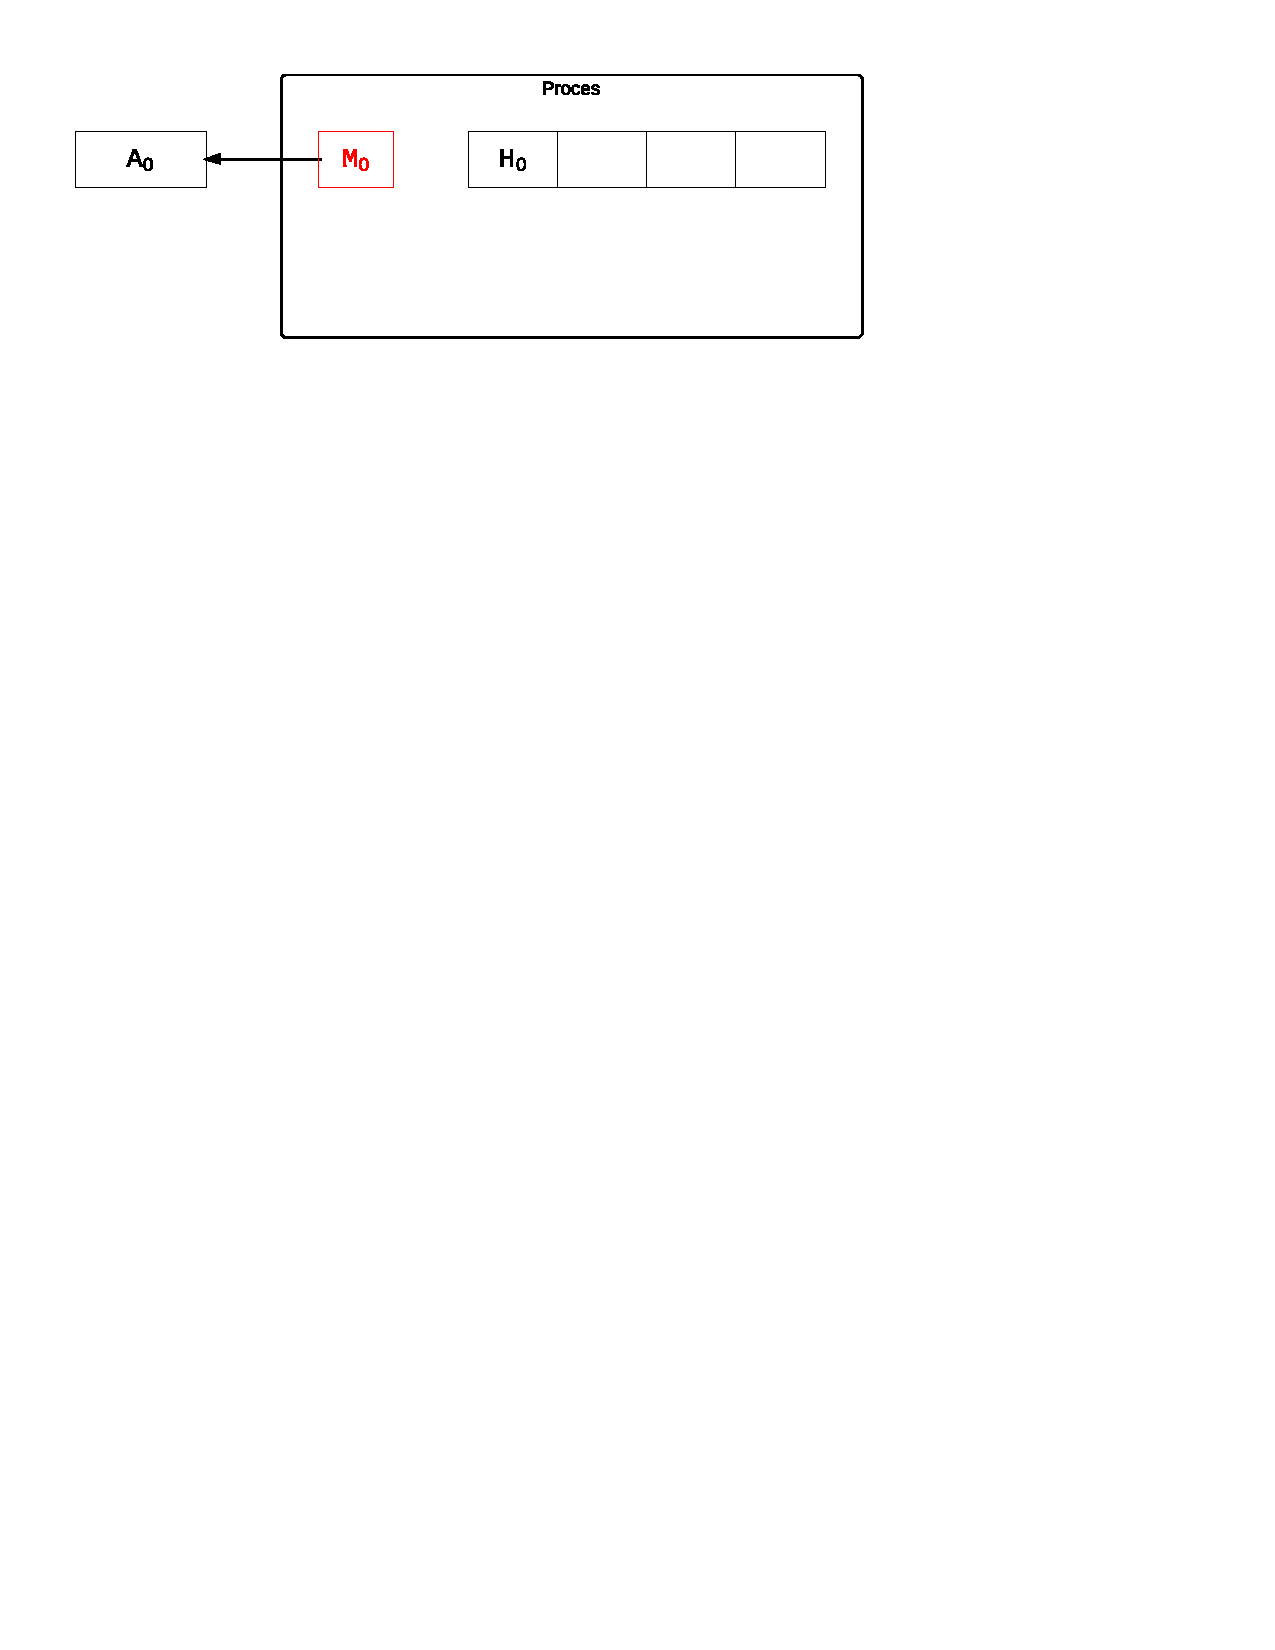
\includegraphics[scale=0.75, clip, trim=10mm 220mm 68mm 10mm]{mp1}}
\caption{Kolejka wiadomości procesu z jedną, nieodczytaną wiadomością.}
\label{fig:mp1}
\end{figure}

Wysłanie wiadomości do procesu polega na dołączeniu na koniec kolejki (która zaimplementowana jest jako lista jednokierunkowa) nowej wiadomości (rys. \ref{fig:mp2}).
Jeżeli wysyłane wyrażenie nie jest bezpośredniego typu danych, całe wyrażenie jest kopiowane do obszaru pamięci poza pamięcią należącą do procesu-odbiorcy.
Wiadomość nie jest kopiowana bezpośrednio na stertę procesu, gdyż w sytuacji w której na stercie nie byłoby wystarczającej ilości miejsca, konieczne byłoby uruchomienie \emph{garbage collectora}.
Tutaj pamięć zajmowana przez treść wiadomości została oznaczona przez \textbf{A\textsubscript{0}} oraz \textbf{A\textsubscript{1}}.
Jego uruchomienie powinno jednak zawsze mieć miejsce w bezpiecznym miejscu kodu, w którym znany jest cały źródłowy zbiór wyrażeń.


\begin{figure}[h]
\centerline{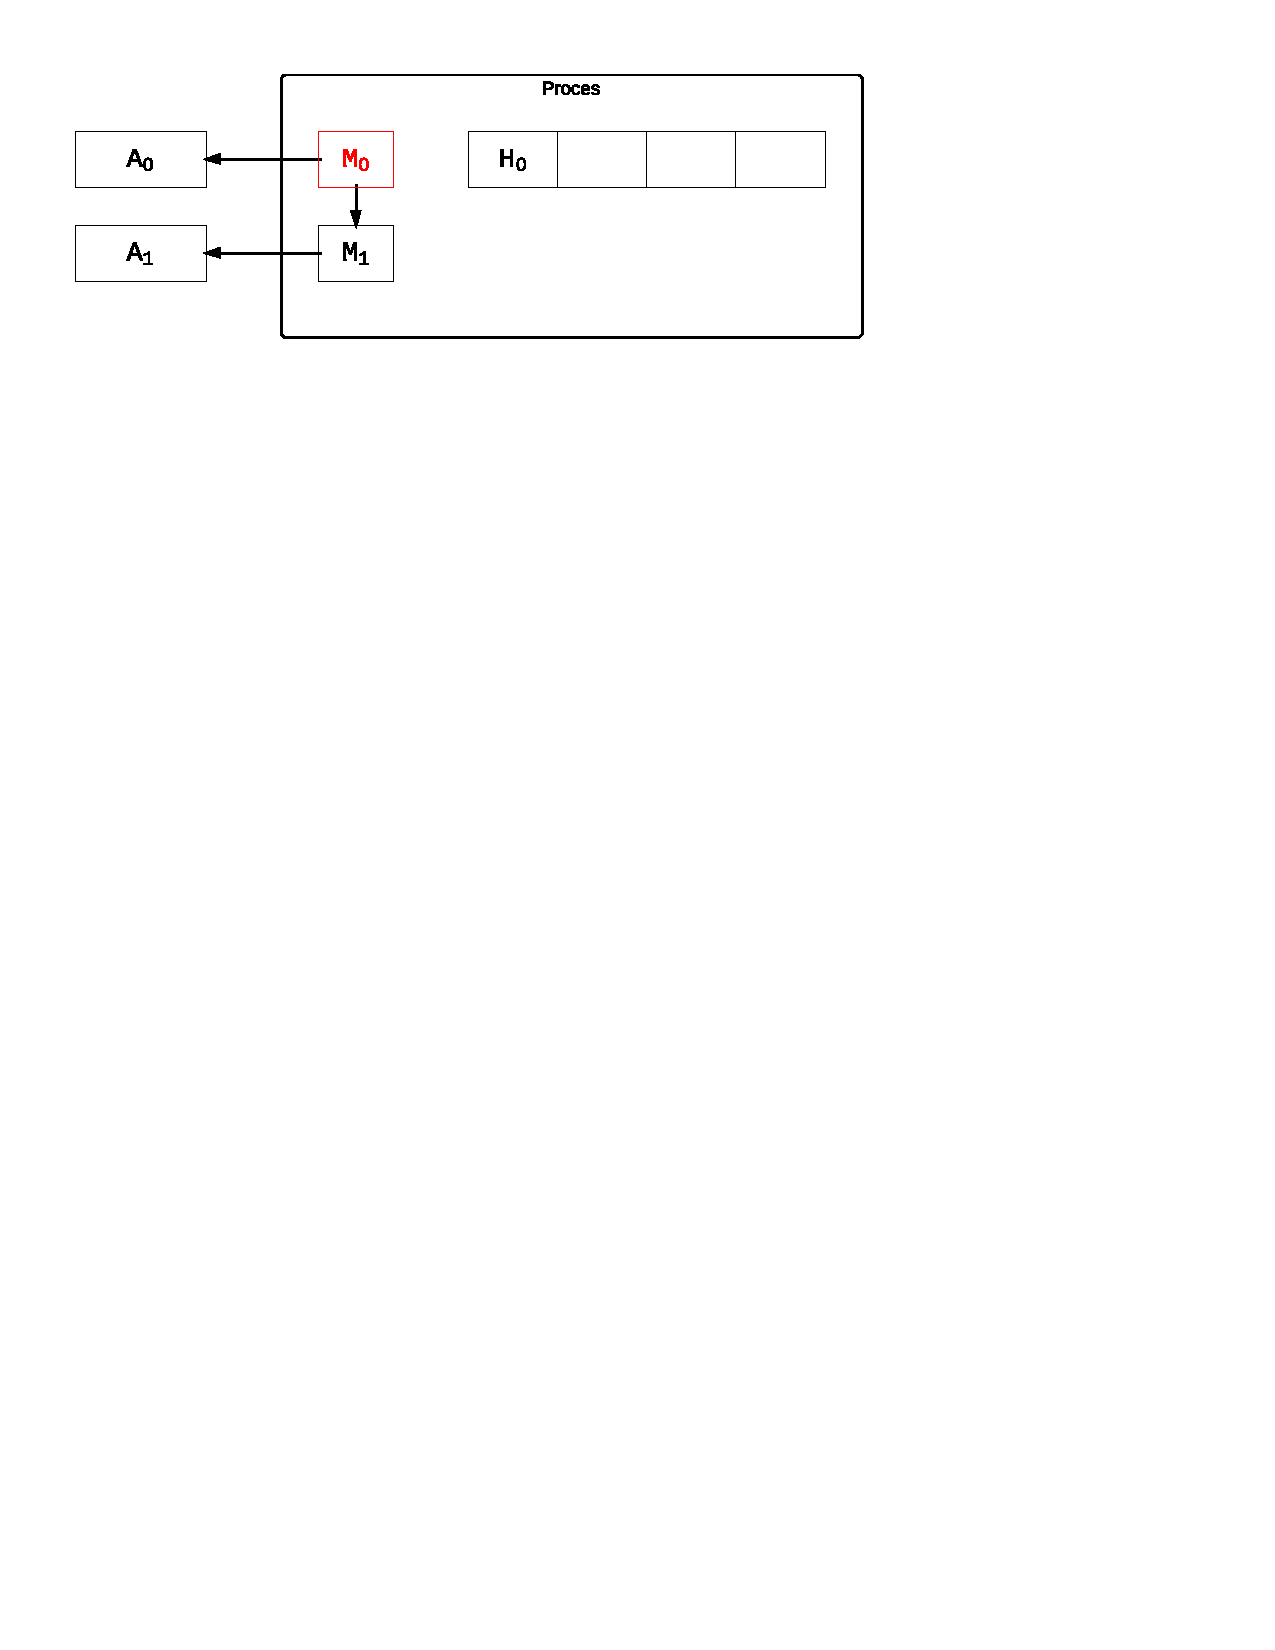
\includegraphics[scale=0.75, clip, trim=10mm 220mm 68mm 10mm]{mp2}}
\caption{Kolejka wiadomości procesu z dodaną kolejną wiadomością.}
\label{fig:mp2}
\end{figure}

W momencie, gdy proces-odbiorca w wykonywanym przez siebie kodzie dochodzi do instrukcji \texttt{loop\_rec} pobierana jest przez niego wiadomość oznaczona wskaźnikiem aktualnej wiadomości. W~sytuacji, gdy kolejka jest pusta proces zostaje zawieszany aż do momentu otrzymania kolejnej wiadomości lub zrealizowania się przeterminowania.
W pierwszym przypadku proces ponownie próbuje pobrać wiadomość z kolejki, w drugim zaś wykonywany jest kod przewidziany po zajściu przeterminowania.

Odebranie wiadomości przez proces polega na skopiowaniu jego zawartości na własną stertę (wyrażenie \textbf{H\textsubscript{1}} na rys. \ref{fig:mp3}), zwolnieniu pamięci zajmowanej przez jej oryginalną zawartość, usunięciu wiadomości z kolejki wiadomości oraz przepisaniu wskaźnika aktualnej wiadomości na następną w kolejce (rys. \ref{fig:mp4}).
Cała procedura jest powtarzana w momencie ponownego dojścia do instrukcji \texttt{loop\_rec} w~kodzie maszynowym (bloku \texttt{receive}).

\begin{figure}[h]
\centerline{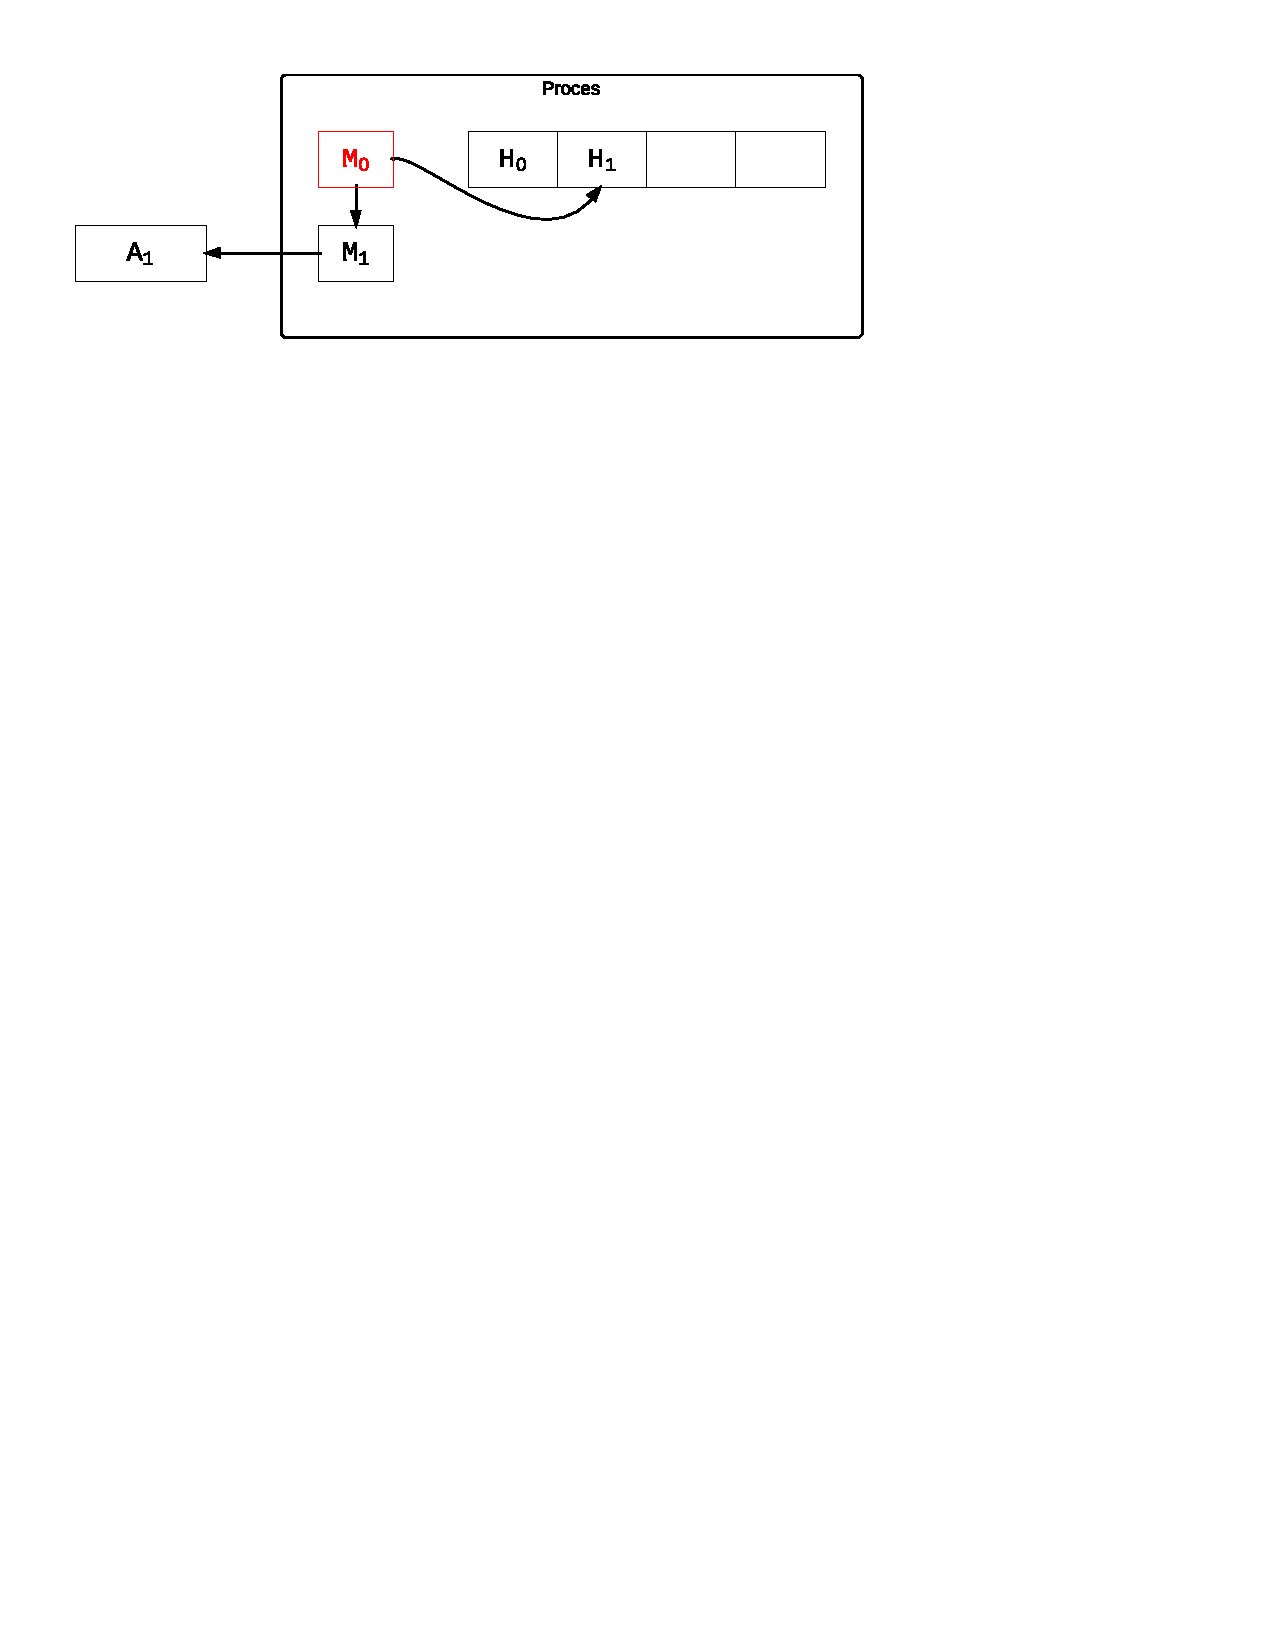
\includegraphics[scale=0.75, clip, trim=10mm 220mm 68mm 10mm]{mp3}}
\caption{Kolejka wiadomości procesu z odczytaną pierwszą wiadomością.}
\label{fig:mp3}
\end{figure}

\begin{figure}[h]
\centerline{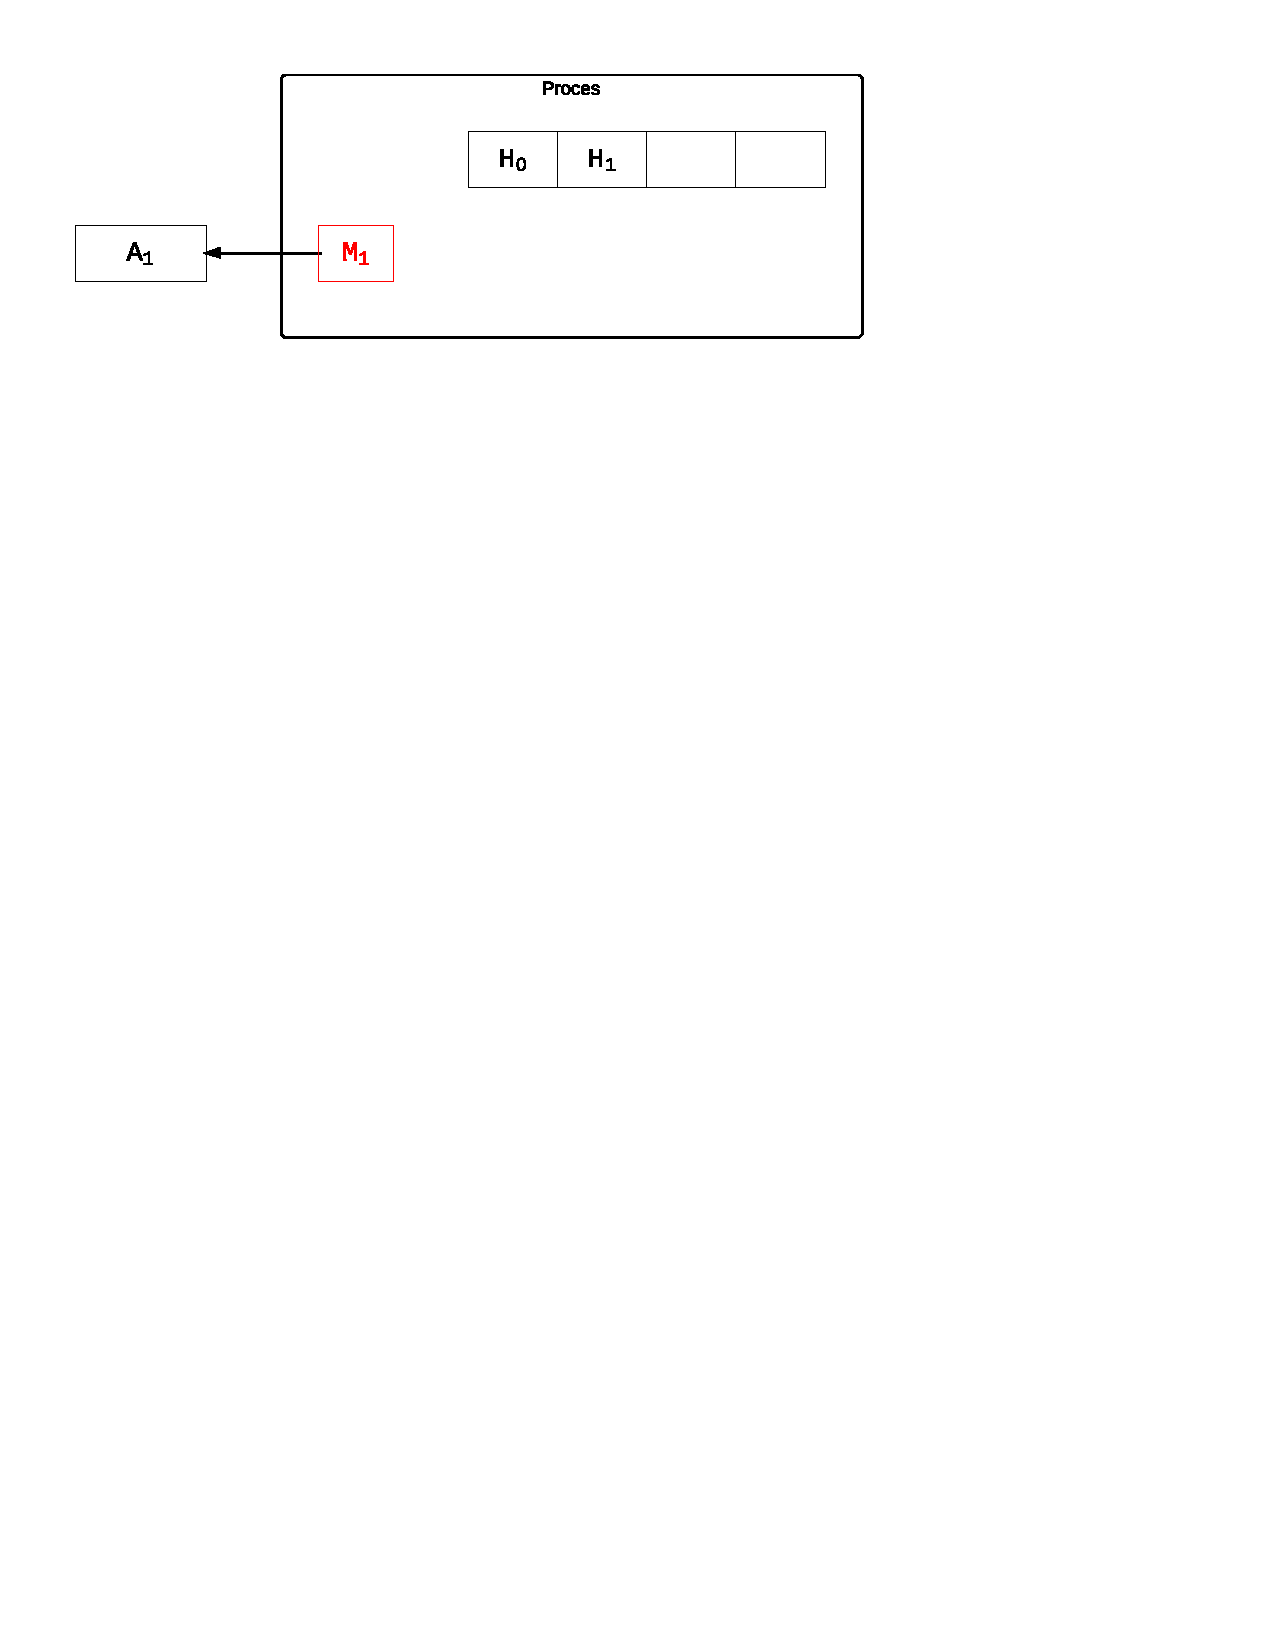
\includegraphics[scale=0.75, clip, trim=10mm 220mm 68mm 10mm]{mp4}}
\caption{Kolejka wiadomości procesu po usunięciu pierwszej wiadomości.}
\label{fig:mp4}
\end{figure}

\subsection{Obsługa błędów}
\label{sub:procBledy}

Maszyna wirtualna opisywana w niniejszej pracy posiada mechanizm dwukierunkowego połączenia procesów (\emph{link}), który zapewnia propagację błędu, w sytuacji gdy w trakcie wykonywania się jednego z~połączonych procesów wystąpi błąd, na skutek którego jego działanie zostanie zakończone.
Domyślnym zachowaniem procesu otrzymującego informację o zakończeniu działania procesu jest w takiej sytuacji jego zakończenie z takim samym błędem.
Możliwe jest jednak ustawienie w nim flagi \texttt{trap\_exit}, czego efektem jest zamiana ww. sygnału na wiadomość wysłaną do tego procesu.

Maszyna wirtualna BEAM oprócz ww. mechanizmu zapewnia również mechanizm jednokierunkowej obserwacji procesów (\emph{monitor}), a także bloki przechwytywania błędów w kodzie (\texttt{try} i \texttt{catch}).
Funkcjonalności te nie zostały jednak zapewnione w maszynie zaimplementowanej w ramach niniejszej pracy.

Lista błędów, jakie mogą wystąpić w trakcie uruchomienia procesu, wraz z opisem sytuacji w jakiej mogą wystąpić została zawarta w dokumentacji języka \cite{ErlangErrors}.

%---------------------------------------------------------------------------
\section{Planista (\emph{scheduler})}
\label{sec:maszynaScheduler}

W systemie współbieżnym procesy mogą działać na jeden z dwóch sposobów:
\begin{itemize}
\item we współbieżności konkurencyjnej (\emph{pre-emptive}), w której planista decyduje o tym kiedy przerwać wykonywanie pewnego procesu i wznowić inne;
\item we współbieżności współpracującej (\emph{cooperative}), w której proces decyduje kiedy przerwać swoje wykonywanie po to, aby \emph{scheduler} mógł wybrać inny proces do wykonania.
\end{itemize}

Z punktu widzenia programisty Erlanga procesy uruchomione w ramach systemu działają we współbieżności konkurencyjnej, gdyż planista sam zarządza kolejką procesów przeznaczonych do wykonania.
Implementacja logiki procesu w maszynie wirtualnej opiera się jednak na współbieżności współpracującej, ponieważ to ona jest odpowiedzialna za wywołanie funkcji wybierającej kolejny proces do wykonania w odpowiedniej chwili. Wynika to z faktu, że wywłaszczenie aktualnie wykonywanego procesu może nastąpić tylko pod pewnymi warunkami.

Pierwszym z nich jest spadek licznika redukcji w danym procesie do zera.
Redukcja jest pojęciem wprowadzonym na potrzeby działania \emph{schedulera} w maszynie wirtualnej BEAM.
Jedna redukcja to wywołanie jednej funkcji (zewnętrznej lub wewnętrznej, operacja z rodziny \textbf{CALL\_*}).
Domyślnie, w maszynie BEAM, gdy \emph{scheduler} wznawia działanie procesu, ten dostaje możliwość wykonania 2000 redukcji zanim będzie musiał oddać dostęp do mocy obliczeniowej innemu procesowi.
W maszynie zaimplementowanej w pracy, ze względu na mniejszą moc obliczeniową docelowej platformy, wartość ta została zmniejszona do 300, podlega ona jednak konfiguracji.
Aby nie doprowadzić do sytuacji, w której można zauważyć znaczącą rozbieżność w czasie dostępu do procesora pomiędzy różnymi procesami, redukcje liczone są także dla innych operacji.
I tak np. funkcje wbudowane czy uruchomienie \emph{garbage collectora} również modyfikują w pewien arbitralny sposób licznik redukcji w procesie. 

Zmiana wykonywanego procesu może wystąpić tylko przed wywołaniem funkcji (czyli przed instrukcją z rodziny \textbf{CALL\_*}), tj. w chwili gdy mamy pewność że wszystkie lokalne zmienne zapisane są na stosie procesu a rejestry \textbf{X} wypełnione są argumentami funkcji.

Procedura zmiany aktualnie wykonywanego procesu polega na odpowiednim zapamiętaniu struktur interpretera w pamięciu procesu przerywającego swoje działanie i odtworzenie tego samego rodzaju danych z pamięciu procesu, który swoje działanie wznawia.
Została ona zaprezentowana na rysunku \ref{fig:preemption}.
Wstrzymywane jest działanie procesu 1, w którego strukturze zapamiętywane są argumenty funkcji którą miał właśnie wywołać.
Zapisywany jest także wskaźnik na szczyt jego stosu oraz wskaźniki instrukcji i~adres powrotu. Na rysunku symbolicznie zostało to oznaczone czerownymi strzałkami.
Proces 2 z kolei wznawia swoje wykonanie. Licznik redukcji zostaje ustawiony ponownie na 300 i wykonywane są operacje odwrotne niż w przypadku procesu 1.
Oznaczone one zostały symbolicznie strzałkami w kolorze zielonym.

\begin{figure}[h]
\centerline{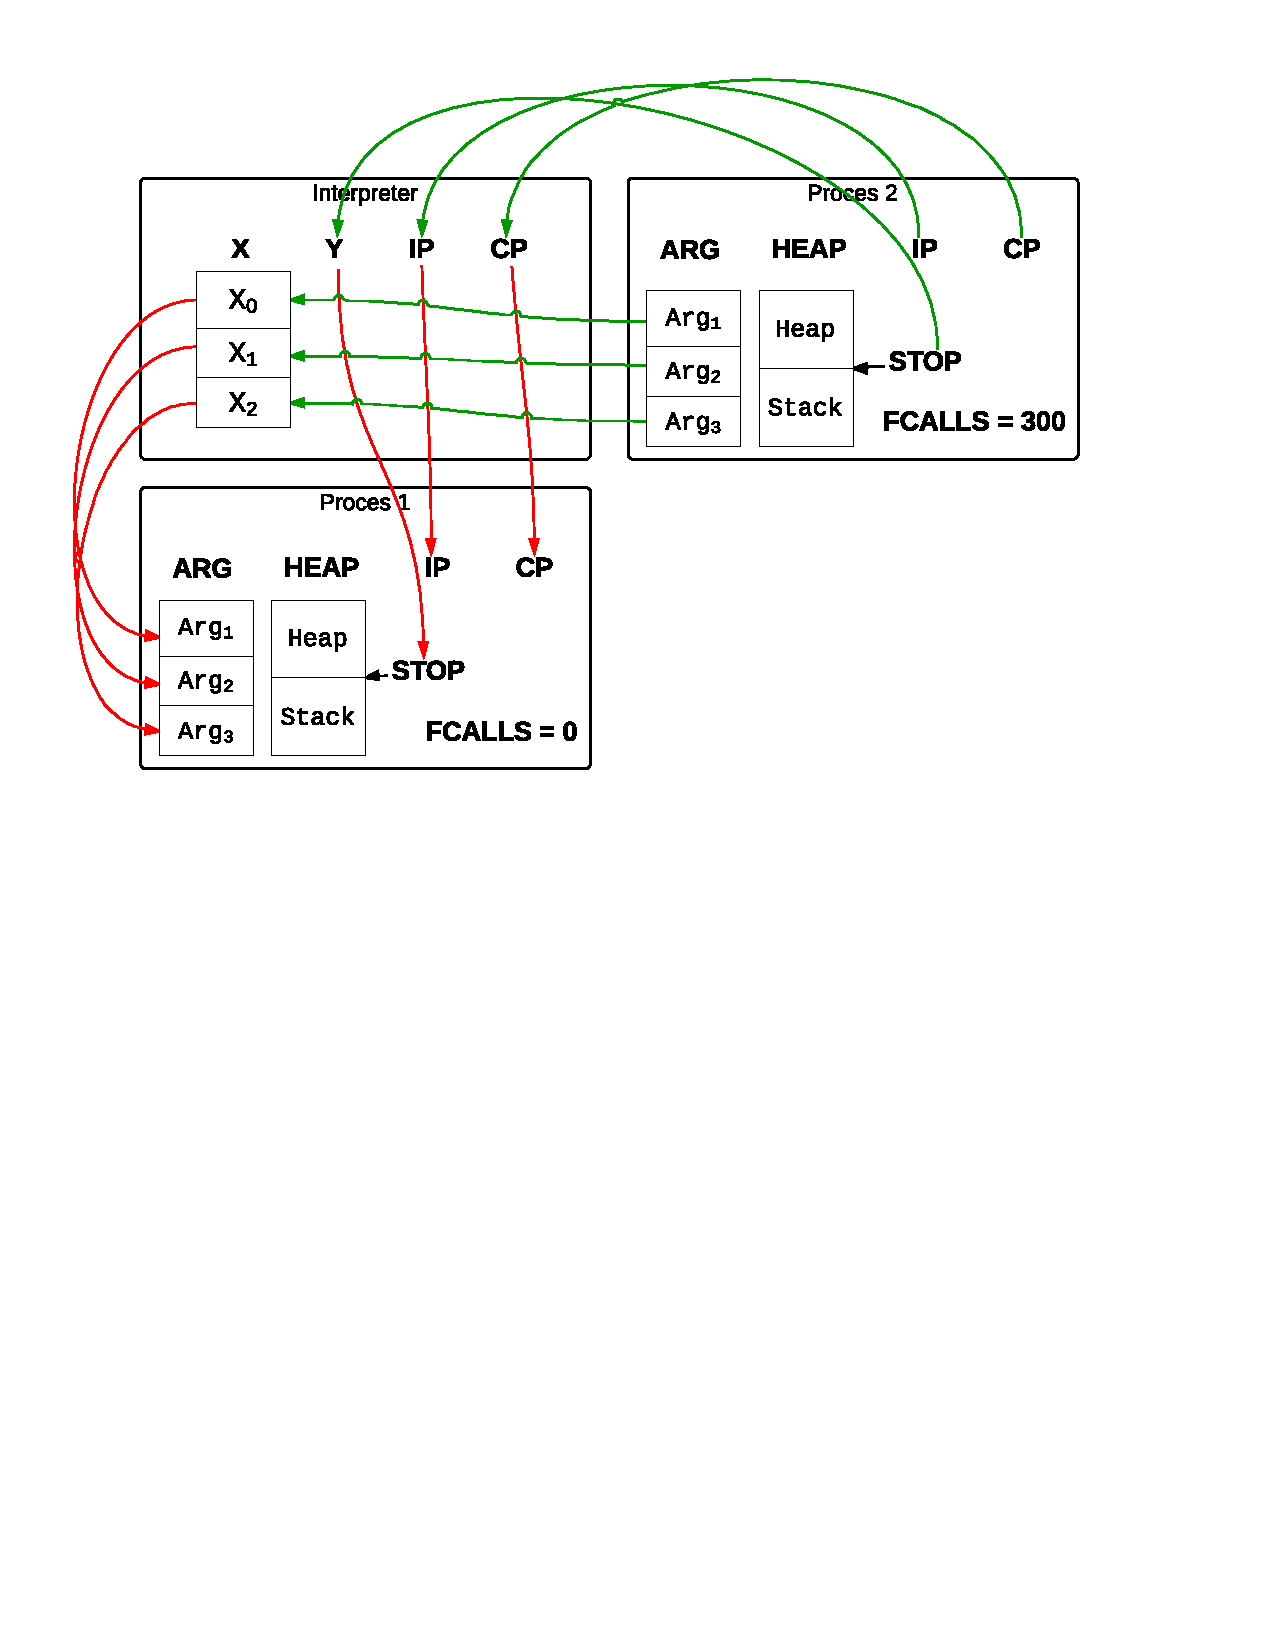
\includegraphics[scale=0.8, clip, trim=10mm 145mm 30mm 10mm]{preemption}}
\caption{Operacje wykonywane w trakcie zmiany wykonywanego procesu}
\label{fig:preemption}
\end{figure}

Istnieje możliwość uruchomienia maszyny wirtualnej BEAM w architekturze SMP (\emph{Symmetric Multiprocessing}), co domyślnie powoduje uruchomienie jednej instancji \emph{schedulera} na jednym fizycznym wątku procesora.
Synchronizację między planistami zapewniają w niej skomplikowane mechanizmy będące przedmiotem ciągłej optymalizacji.
Maszynę zaimplementowaną w pracy można uruchomić jednak tylko z~wykorzystaniem tylko jednego fizycznego wątku.
Pomimo badań nad uruchomieniem \emph{schedulera} mikrojądra FreeRTOS na architekturze wielordzeniowej \cite{Mistry2011}, oficjalna dystrybucja wspiera obecnie tylko architekturę jednordzeniową.

Maszyna wirtualna BEAM posiada zaimplementowane priorytety procesów: \textbf{max}, \textbf{high}, \textbf{normal} oraz \textbf{low}.
Procesy domyślnie uruchomiane są z priorytetem \textbf{normal}. 
Planista, w momencie gdy licznik redukcji aktualnie wykonywanego procesu osiągnie wartość 0 lub proces będzie oczekiwał na wiadomość w bloku \texttt{receive}, dokona wyboru kolejnego procesu do wykonania.

Proces może zostać wybrany spośród trzech dostępnych kolejek zawierających procesy o priorytecie:
\begin{itemize}
\item \textbf{max} --- jeżeli w kolejce jest zakolejkowany przynajmniej jeden proces to jest będzie on wybranym jako kolejny do wykonania;
\item \textbf{high} --- jeżeli kolejka procesów o priorytecie \textbf{max} jest pusta a w tej kolejce znajduje się przynajmniej jeden proces to zostanie on wybrany do uruchomienia;
\item \textbf{normal} i \textbf{low} --- kolejka zawiera procesy o dwóch priorytetach, jednak procesy o priorytecie \textbf{low} zawierają specjalny licznik, który wskazuje na to ile razy proces musi zostać pominięty przy wyborze do uruchomienia zanim faktycznie zostanie uruchomiony. Wartość licznika dla tego rodzaju procesów po zakolejkowaniu wynosi 8. Procesy z tej kolejki mogą zostać wybrane do wznowienia przez \emph{scheduler} tylko w sytuacji gdy kolejki z procesami o priorytetach \textbf{max} i \textbf{high} są puste.
\end{itemize}

Aktualny proces umieszczany jest na końcu kolejki odpowiadającej swojemu priorytetowi od razu (jeżeli zostaje zatrzymany z powodu wyczerpania się dostępnych redukcji) lub po otrzymaniu wiadomości lub przeterminowaniu (jeśli został zatrzymany na skutek wejścia w blok \texttt{receive}).

Wersja maszyny wirtualnej zaimplementowanej w pracy nie implementuje możliwości zmiany priorytetu uruchomionego procesu.
Wszystkie procesy uruchamiane są z takim samym priorytetem.
Jest to jednak funkcjonalność, której implementacja jest godna rozważenia w trakcie dalszego rozwoju projektu, biorąc pod uwagę fakt, że mikrojądro FreeRTOS pozwala na wybór priorytetu zadania a działanie planisty systemu jest bardzo podobne do ww. mechanizmu działania \emph{schedulera} maszyny wirtualnej BEAM.

%---------------------------------------------------------------------------
\section{Funkcje wbudowane (\emph{Built-In Functions})}
\label{sec:maszynaBIF}

W niniejszym podrozdziale zaprezentowano zbiór zaimplementowanych funkcji wbudowanych w~maszynę wirtualną dla systemu FreeRTOS.
Z punktu widzenia programisty funkcja wbudowana jest zwykłą funkcją zaimplementowaną w zewnętrznym module, jej implementacja jest jednak częścią kodu maszyny wirtualnej w języku C.
Nie jest zatem wykonywana ona jako kod pośredni przez interpreter, ale jako kod maszynowy danej architektury, co wpływa pozytywnie na szybkość jej wykonania.
Każdej funkcji wbudowanej odpowiada wpis w tablicy funkcji eksportowanych, podobnie jak funkcjom eksportowanym z załadowanych modułów.
Wpis ten zamiast wskaźnika do instrukcji kodu maszynowego do wykonania zawiera wskaźnik do funkcji zaimplementowanej w języku C.

\subsection{Funkcje ogólne (moduł \texttt{erlang})}
\label{sub:bifErlang}
Funkcje opisane w tej części podrozdziału zostały zaimplementowane w pliku źródłowym \texttt{erl\_bif.c}.

\begin{longtable}{|c|c|p{7.5cm}|}
\hline

Funkcja & Argumenty & Opis \\
\endfirsthead
\hline
\texttt{splus/2} & \texttt{Arg1 Arg2} & Zwraca \texttt{Arg1 + Arg2} \\
\hline
\texttt{sminus/2} & \texttt{Arg1 Arg2} & Zwraca \texttt{Arg1 - Arg2} \\
\hline
\texttt{stimes/2} & \texttt{Arg1 Arg2} & Zwraca \texttt{Arg1 * Arg2} \\
\hline
\texttt{spawn/3} & \texttt{M F A} & Startuje nowy proces, wykonujący funkcję \texttt{F} w~module \texttt{M} z listą argumentów \texttt{A} \\
\hline
\texttt{spawn\_link/3} & \texttt{M F A} & Startuje nowy proces, wykonujący funkcję \texttt{F} w~module \texttt{M} z listą argumentów \texttt{A}. Łączy wystartowany proces z wywołującym \emph{linkiem}.\\
\hline
\texttt{setelement/3} & \texttt{Index Tuple Element} & Zwraca nową krotkę, taką jak \texttt{Tuple}, ale z elementem \texttt{Element} na pozycji \texttt{Index} \\
\hline
\texttt{now/0} & & Zwraca krotkę \texttt{\{M,S,U\}} zawierająca kolejną liczbę megasekund, sekund i mikrosekund jakie upłynęły od uruchomienia maszyny wirtualnej \\
\hline
\texttt{length/1} & \texttt{List} & Zwraca długość listy \texttt{List} \\
\hline
\texttt{plusplus/2} & \texttt{List1 List2} & Zwraca nową listę, stanowiącą złączenie list \texttt{List1} i \texttt{List2} \\
\hline
\texttt{div/2} & \texttt{Int1 Int2} & Zwraca wynik dzielenia całkowitoliczbowego argumentów \\
\hline
\texttt{rem/2} & \texttt{Int1 Int2} & Zwraca resztę z dzielenia argumentów \\
\hline
\texttt{bsr/2} & \texttt{Int1 Int2} & Zwraca wynik przesunięcia bitowego w prawo argumentów \\
\hline
\texttt{band/2} & \texttt{Int1 Int2} & Zwraca iloczyn logiczny argumentów \\
\hline
\texttt{bor/2} & \texttt{Int1 Int2} & Zwraca alternatywę logiczną argumentów \\
\hline
\texttt{element/2} & \texttt{N Tuple} & Zwraca \texttt{N}-ty element krotki \texttt{Tuple} \\
\hline
\texttt{exit/1} & \texttt{Reason} & Kończy działanie wywołującego procesu z powodem \texttt{Reason} \\
\hline
\texttt{process\_flag/2} & \texttt{trap\_exit true} & Wywołujący proces nie kończy działania gdy kończą działania procesy połączone, ale otrzymuje informacje o tym fakcie w postaci wiadomości \\
\hline
\texttt{self/0} & & Zwraca \textbf{PID} wywołującego procesu \\
\hline
\texttt{send\_after/3} & \texttt{Time Dest Mesg} & Ustawia przeterminowanie wysyłające wiadomość \texttt{Mesg} do procesu \texttt{Dest} za \texttt{Time} milisekund. \\
\hline
\caption{Zaimplementowane funkcje wbudowane w module \texttt{erlang}} 
\label{table:bifErlang} \\
\end{longtable}


\subsection{Listy (moduł \texttt{lists})}
\label{sub:bifLists}

Funkcje opisane w tej części podrozdziału zostały zaimplementowane w pliku źródłowym \texttt{erl\_bif\_lists.c}.

\begin{longtable}{|c|c|p{8cm}|}
\hline

Funkcja & Argumenty & Opis \\
\endfirsthead
\hline
\texttt{reverse/1} & \texttt{List} & Zwraca nową listę bedącą odwróconą listą \texttt{List} \\
\hline
\caption{Zaimplementowane funkcje wbudowane w module \texttt{lists}} 
\label{table:bifLists} \\
\end{longtable}

\subsection{GPIO i obsługa przerwań (moduł \texttt{lpc\_gpio})}
\label{sub:bifGPIO}
Funkcje opisane w tej części podrozdziału zostały zaimplementowane w pliku źródłowym \texttt{erl\_bif\_lpc.c}.

\begin{longtable}{|c|c|p{10cm}|}
\hline

Funkcja & Argumenty & Opis \\
\endfirsthead
\hline
\texttt{output/2} & \texttt{Port Pin} & Ustawia pin \texttt{Pin} na porcie \texttt{Port} mikrokontrolera w tryb wyjścia\\
\hline
\texttt{high/2} & \texttt{Port Pin} & Ustawia stan wysoki na pinie \texttt{Pin} na porcie \texttt{Port} \\
\hline
\texttt{low/2} & \texttt{Port Pin} & Ustawia stan niski na pinie \texttt{Pin} na porcie \texttt{Port} \\
\hline
\texttt{interrupt/3} & \texttt{0 Pin falling} & Subskrybuje proces na opadające zbocze na pinie \texttt{Pin} na porcie \texttt{0}. Informacja  o przerwaniu dotrze do procesu w postaci wiadomości w postaci \texttt{interrupt}.\\
\hline
\caption{Zaimplementowane funkcje wbudowane w module \texttt{lpc\_gpio}} 
\label{table:bifGpio} \\
\end{longtable}


\subsection{SPI (moduł \texttt{lpc\_spi})}
\label{sub:bifSPI}

Funkcje opisane w tej części podrozdziału zostały zaimplementowane w pliku źródłowym \texttt{erl\_bif\_spi.c}.

\begin{longtable}{|c|c|p{10cm}|}
\hline

Funkcja & Argumenty & Opis \\
\endfirsthead
\hline
\texttt{init/1} & \texttt{Frequency} & Inicjalizuje interfejs SPI mikrokontrolera w trybie \emph{master} z sygnałem zegarowym o częstotiwości \texttt{Frequency} \\
\hline
\texttt{rw/1} & \texttt{Byte} & Wysyła bajt \texttt{Byte} po interfejsie SPI. Wartością zwracaną jest bajt otrzymany z interfejsu w trakcie transmisji. \\
\hline
\caption{Zaimplementowane funkcje wbudowane w module \texttt{lpc\_spi}} 
\label{table:bifSpi} \\
\end{longtable}

\subsection{Funkcje pomocnicze (moduł \texttt{lpc\_debug})}
\label{sub:bifDebug}
Funkcje opisane w tej części podrozdziału zostały zaimplementowane w pliku źródłowym \texttt{erl\_bif\_lpc.c}.

\begin{longtable}{|c|c|p{10cm}|}
\hline

Funkcja & Argumenty & Opis \\
\endfirsthead
\hline
\texttt{dump\_regs/0} &  & Drukuje zawartość rejestrów X\\
\hline
\texttt{dump\_stack/0} &  & Drukuje zawartość stosu wywołującego procesu\\
\hline
\texttt{dump\_heap/0} &  & Drukuje zawartość sterty wywołującego procesu\\
\hline
\texttt{print\_info/0} &  & Drukuje informacje dotyczące wywołującego procesu\\
\hline
\texttt{print\_term/1} & \texttt{Term}  & Drukuje zawartość wyrażenia \texttt{Term} \\
\hline
\caption{Zaimplementowane funkcje wbudowane w module \texttt{lpc\_debug}} 
\label{table:bifDebug} \\
\end{longtable}

%---------------------------------------------------------------------------
\section{\emph{Garbage collector}}
\label{sec:maszynaGC}

Moduł opisany w niniejszym podrozdziale został zaimplementowany w pliku źródłowym \texttt{erl\_gc.c}.

\subsection{Pamięć zajmowana przez proces}
\label{sub:gcHeap}

Blok pamięci zajmowany przez proces do przechowywania wyrażeń których używa nosi nazwę sterty i zarządzany jest automatycznie przez \emph{garbage collector}.
Obszar pamięci ten podzielony jest na dwie części:
\begin{itemize}
\item stertę, służącą do przechowywania danych złożonych (krotki, listy) lub opakowanych (\textbf{BOXED}), z których proces może korzystać nawet przez cały czas swojego życia;
\item stos, którego zadaniem jest zachowywanie informacji pomiędzy wywołaniami funkcji, takich jak zmienne lokalne czy adresy powrotu.
\end{itemize}

Pojęcie sterty jest w niniejszej pracy używane wymiennie w odniesieniu albo do całego zaalokowanego dla procesu bloku pamięci albo do pierwszej wspomnianej jego części.
Proces przechowuje kilka wskaźników dzięki którym możliwa jest identyfikacja odpowiednich fragmentów pamięci i wykonywanie operacji na nich. Należą do nich:
\begin{itemize}
\item \textbf{HEAP}, oznaczający początek całego bloku pamięci, a zarazem i sterty;
\item \textbf{HTOP}, oznaczający koniec sterty;
\item \textbf{STOP}, oznaczający początek stosu;
\item \textbf{HEND}, oznaczający koniec bloku pamięci, a zarazem i stosu.
\end{itemize}
Graficzne odniesienie wskaźników do miejsc w pamięci procesu zostało zaprezentowane na rysunku \ref{fig:heap}. 
Jak można zauważyć, wyrażenia dodawane do sterty procesu umieszczane są począwszy od początku całego bloku pamięci.
Z kolei wyrażenia dodawane na stos umieszczane są od końca bloku, w~kierunku jego początku.
Wskazywanie przez wskaźniki \textbf{HTOP} oraz \textbf{STOP} na to samo miejsce w~pamięci oznacza, że na stercie procesu skończyło się miejsce i konieczne jest uruchomienie \emph{garbage collectora}.

\begin{figure}[h]
\centerline{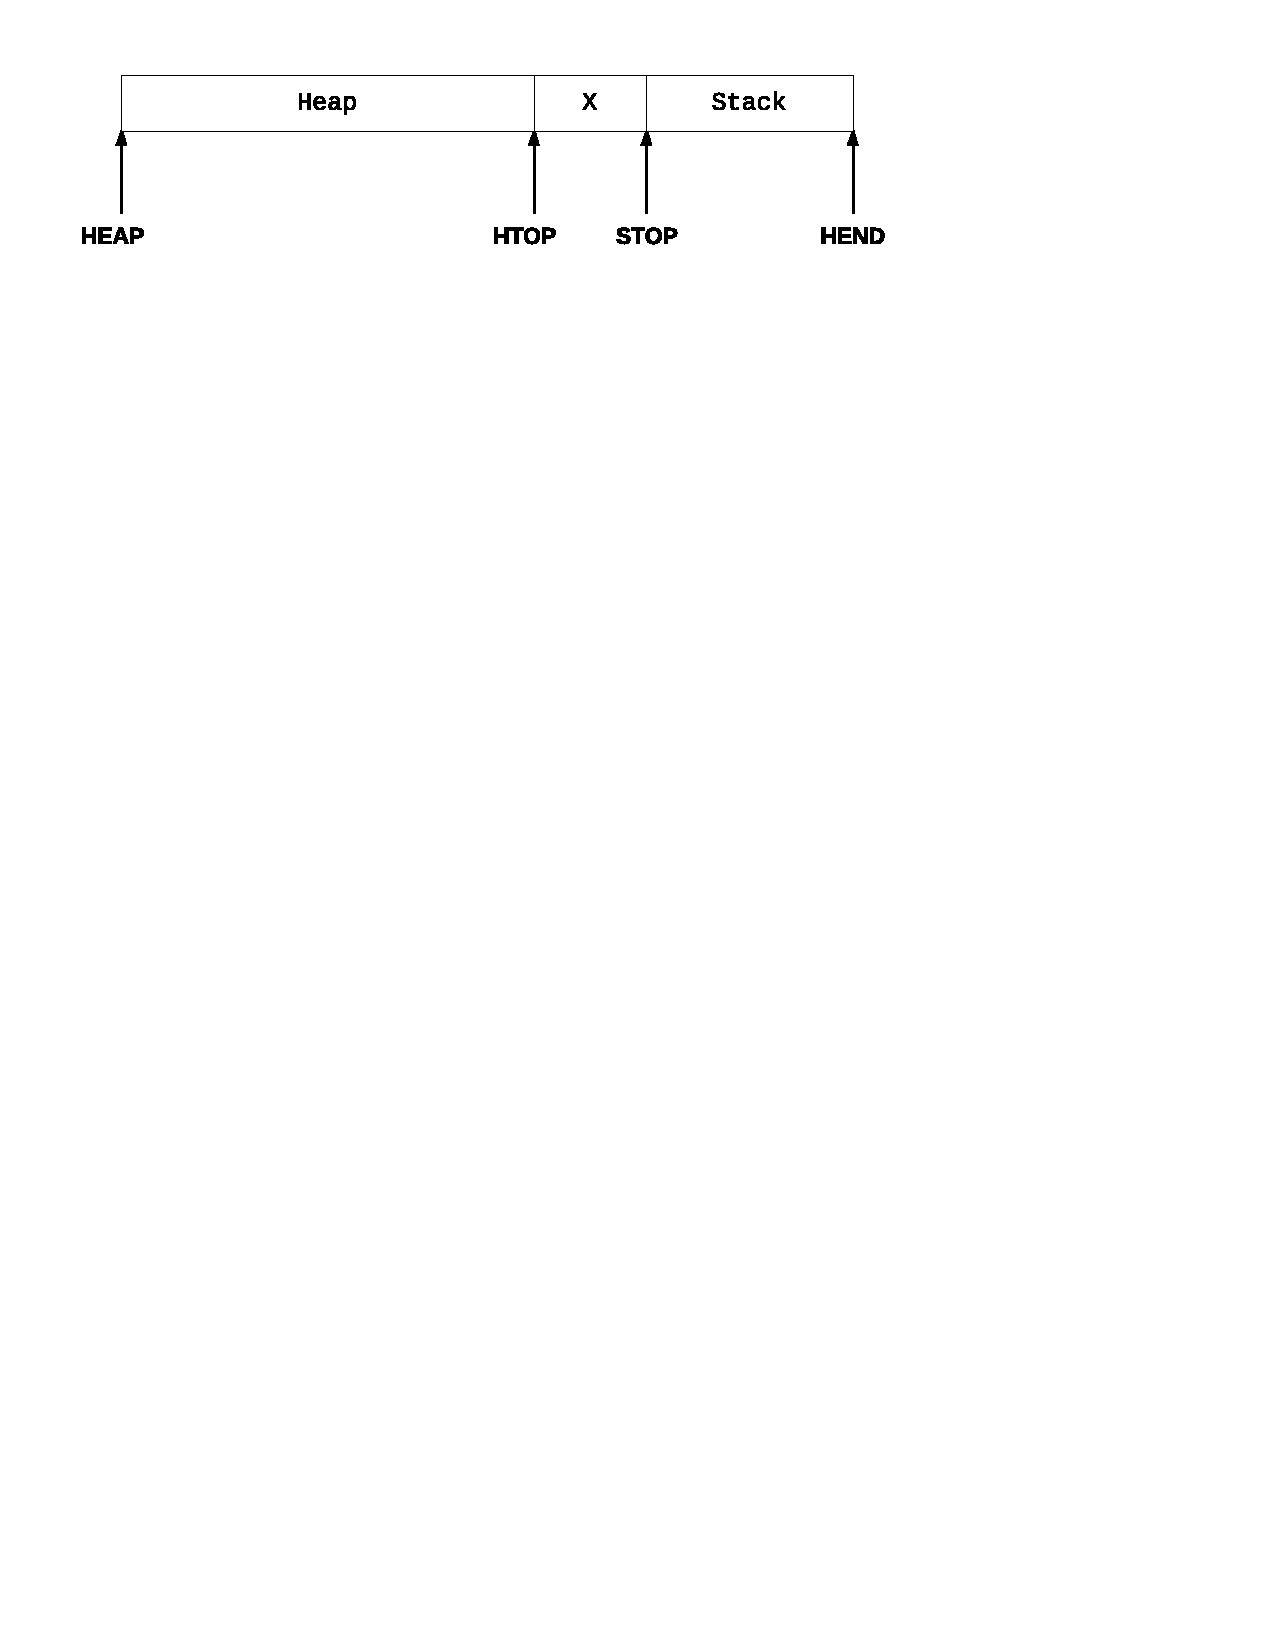
\includegraphics[scale=1, clip, trim=10mm 235mm 65mm 10mm]{heap}}
\caption{Struktura pamięci zajmowanej przez proces wraz ze wskaźnikami na poszczególne struktury}
\label{fig:heap}
\end{figure}

Sterta zaalokowana dla procesu może mieć jeden z pewnych ustalonych z góry rozmiarów, należący do ciągu:

\begin{equation}
h_{n} = \left\lbrace
\begin{array}{rcl}
12 & \text{dla} & n = 1,\\
38 & \text{dla} & n = 2,\\
h_{n-1} + h_{n-2} + 1 & \text{dla} & n > 2
\end{array}
\right.
\end{equation}

Rozmiar ten wyrażony jest w słowach maszynowych i dla maszyny BEAM domyślnie wynosi 233 (6. wyraz ciągu).
W maszynie zaimplementowanej w pracy domyślnym, początkowym rozmiarem sterty procesu jest 12 słów maszynowych ze względu na mniejsze zapotrzebowanie na pamięć, wynikające~z~przeznaczenia aplikacji.

\subsection{Algorytm Cheneya}
\label{sub:gcCheney}

Algorytmem odśmiecania wykorzystywanym w maszynie wirtualnej Erlanga jest algorytm Cheneya \cite{Cheney1970}.
Jest on algorytmem kopiującym, którego działanie polega na zaalokowaniu nowego bloku pamięci i przeniesieniu do niego wszystkich obecnie używanych obiektów.
Kolejnym krokiem jest przepisanie wszystkich istniejących referencji do poprzedniego bloku pamięci.
Na końcu następuje zwolnienie starego bloku pamięci.
Ten prosty algorytm pasuje do filozofii języka, gdzie każdy uruchomiony proces korzysta tylko i wyłącznie z pamięci zajmowanej przez samego siebie.
Dzięki temu możliwe jest uruchamianie \emph{garbage collectora} w kontekście każdego procesu z osobna.
Nie powoduje to zatrzymań działania całego uruchomionego systemu na czas odśmiecania sterty procesu.
Algorytm zostanie uruchomiony w~sytuacji, gdy na stercie nie ma wolnej liczby słów maszynowych potrzebnej do zaalokowania w danej chwili lub zostanie on wywołany \emph{explicite} przez funkcję \texttt{erlang:garbage\_collect/0-2}.

Działanie algorytmu Cheneya uruchomionego w procesie erlangowego zostało zaprezentowano na rysunkach od \ref{fig:gc0} do \ref{fig:gc6}.
Do zilustrowania sposobu działania algorytmu posłużono się abstrakcją trójkolorową, służącą do znalezienia obiektów których pamięć można zwolnić, wykorzystującą do ich oznaczania trzech kolorów:
\begin{itemize}
\item białego, oznaczającego że stan obiektu jest w tym momencie nieznany, ale nie napotkano jeszcze żadnego obiektu odwołującego się do niego;
\item szarego, obiekt jest wykorzystywany i nie można go usunąć, ale nie przetworzono jeszcze obiektów zależnych od niego;
\item czarnego, obiekt, podobnie jak obiekty od niego zależne, są wykorzystywane.
\end{itemize}
Celem algorytmu odśmiecania jest osiągnięcie takiego stanu, w którym wszystkie obiekty będą oznaczone kolorem czarnym (obiekty wykorzystywane) lub białym (obiekty niewykorzystywane które można usunąć z pamięci).
Na początku działania algorytmu, początkowy zbiór wyrażeń oznaczony jest kolorem szarym.
Ze względu na kopiujący charakter algorytmu, kolor obiektów na dotychczasowej stercie procesu będzie zawsze biały.
Obiekty przekopiowane na nową stertę będą z kolei tylko szare lub czarne.

Do początkowego zbioru wyrażeń, które odnosić będą się do używanej pamięci, w zaimplementowanej maszynie należą:
stos procesu, używane rejestry \textbf{X} i kolejka wiadomości (rys. \ref{fig:gc0}). W maszynie wirtualnej BEAM do tego zbioru należy jeszcze kilka innych struktur, jak np. słownik procesu.

\begin{figure}[h]
\centerline{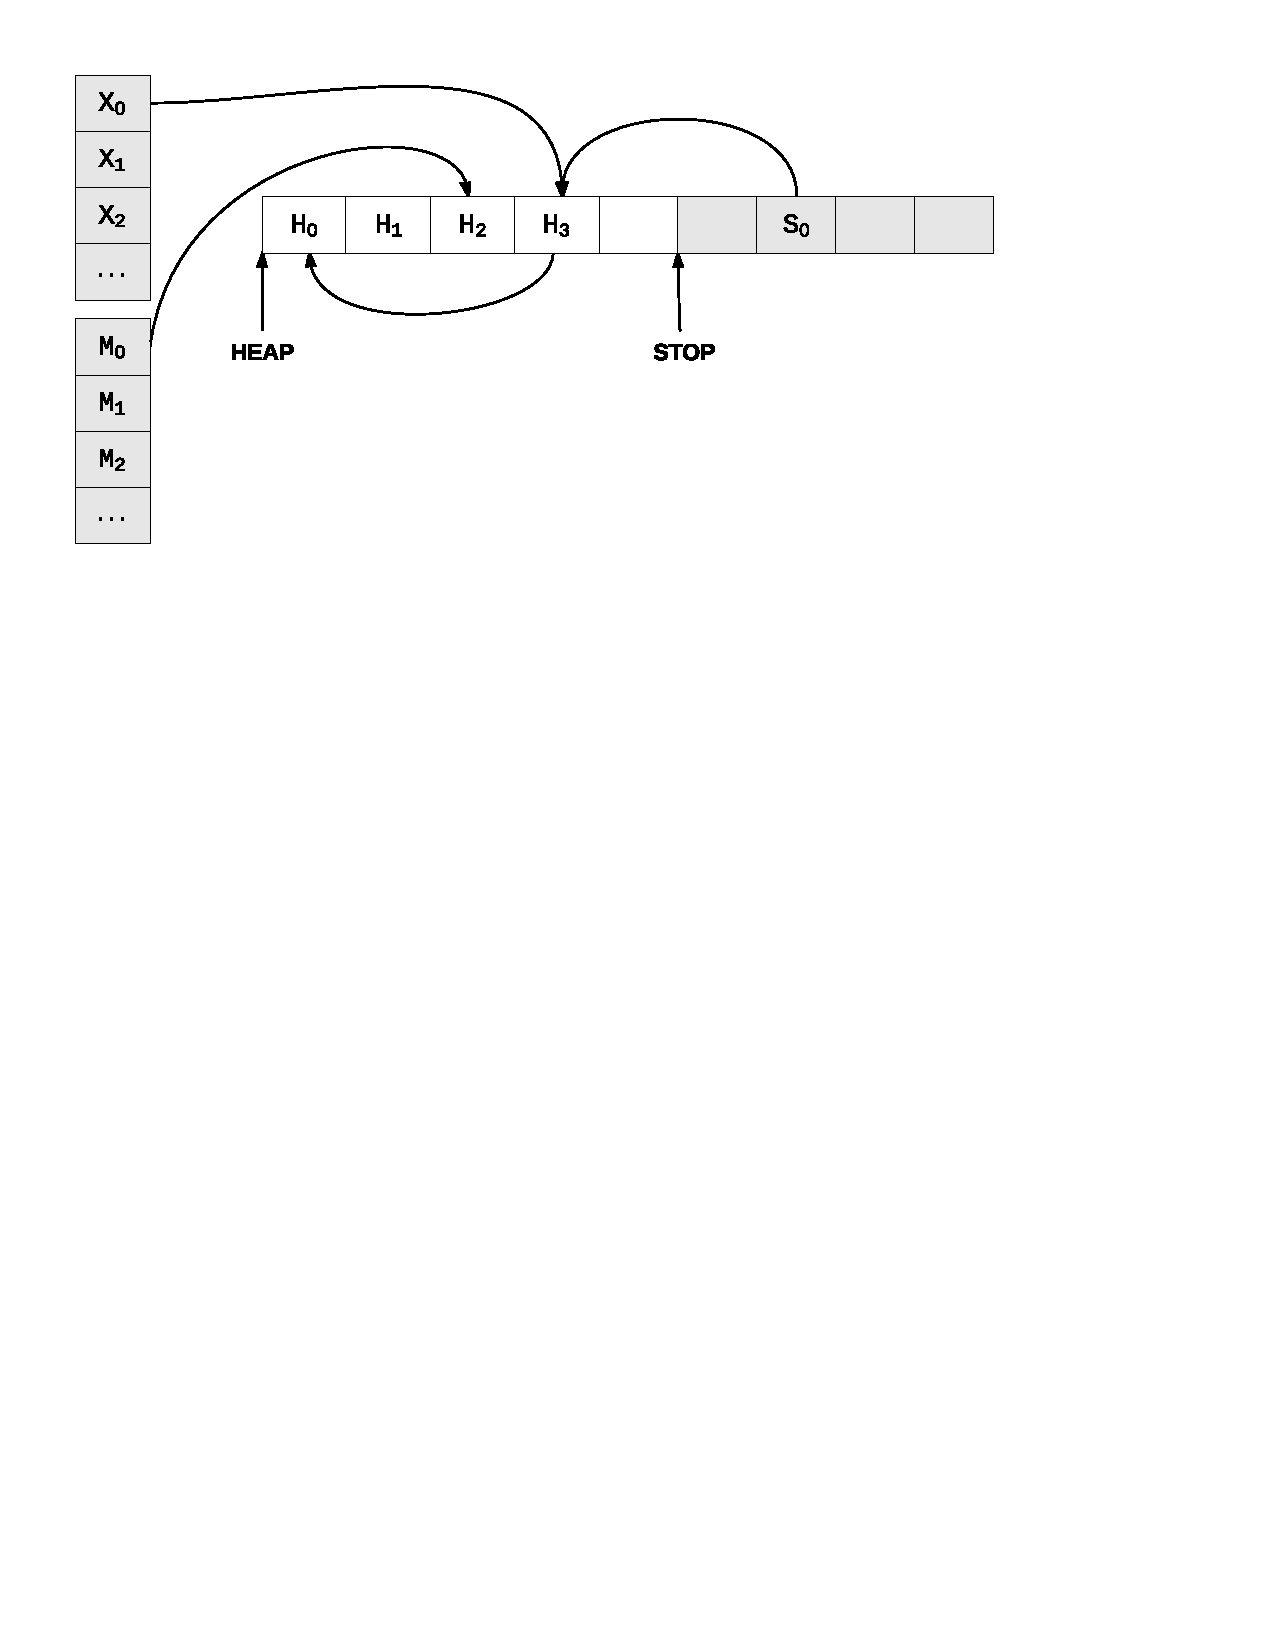
\includegraphics[scale=0.75, clip, trim=10mm 185mm 45mm 10mm]{gc_0}}
\caption{Sterta poddawana odśmiecaniu. Szary zbiór stanowi stos procesu, rejestry \textbf{X} i kolejka wiadomości procesu.}
\label{fig:gc0}
\end{figure}

Pierwszym krokiem działania algorytmu jest zaalokowanie sterty procesu o takiej samej długości jak dotychczasowa (rys. \ref{fig:gc1}).
Następnie przetwarzane są kolejne elementy zbioru szarego, a wyrażenia do których zawierają referencję kopiowane są na nową stertę.
Tak jest w przypadku wyrażenia \textbf{H\textsubscript{3}}, do którego odnosi się rejestr \textbf{X\textsubscript{0}}.
Wyrażenie to zostało przekopiowane na nową stertę i referencja do nowego wyrażenia została zapisana w tym rejestrze.
Obiekt \textbf{H\textsubscript{3}'} miał w tym momencie kolor szary.
Dlatego, że on sam zawierał referencję do wyrażenia \textbf{H\textsubscript{0}}, to wyrażenie także musiało zostać przeniesione na nową stertę.
Przeniesiony obiekt nie zawierał już referencji do żadnego innego obiektu, dlatego zaraz po oznaczeniu go kolorem szarym można było zmienić jego kolor na czarny.

\begin{figure}[h]
\centerline{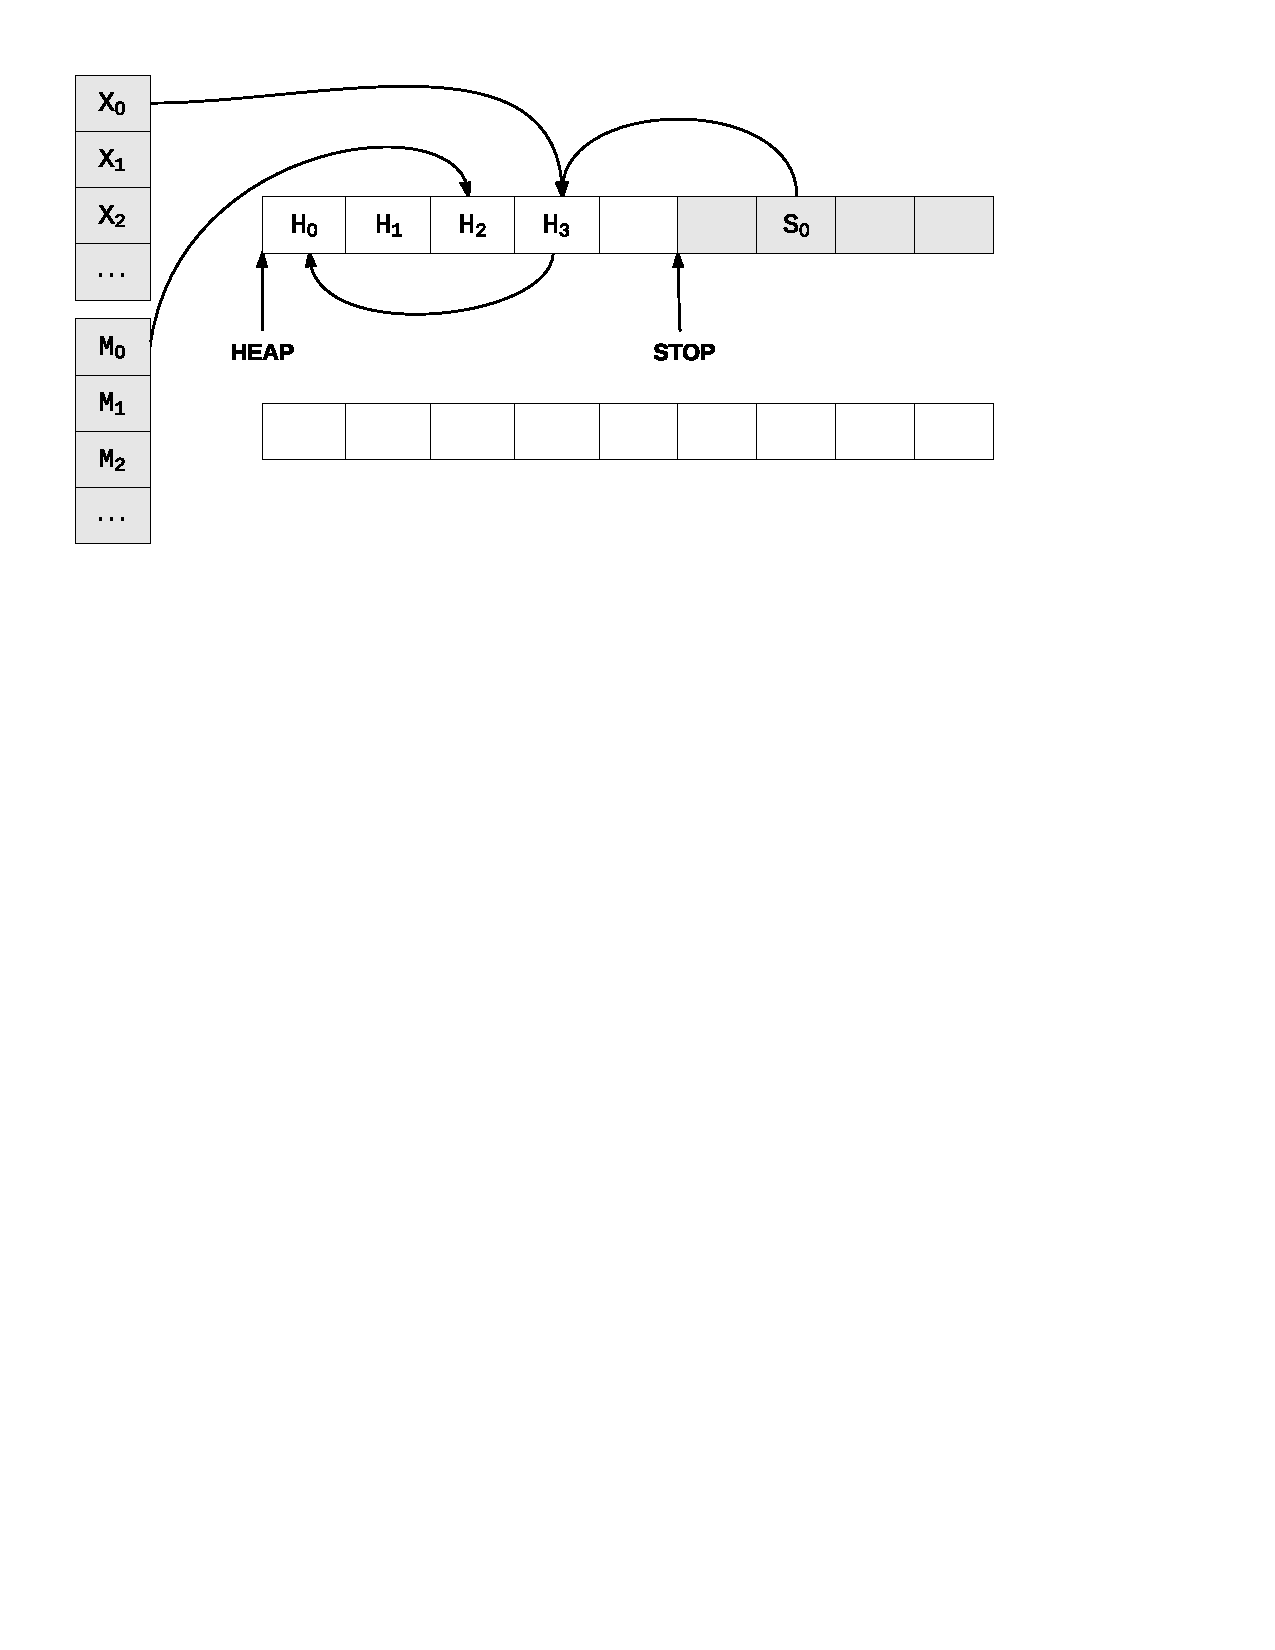
\includegraphics[scale=0.75, clip, trim=10mm 185mm 45mm 10mm]{gc_1}}
\caption{Alokacja nowej sterty o takim samym rozmiarze jak dotychczasowa.}
\label{fig:gc1}
\end{figure}

Dopiero po podmianie referencji w~wyrażeniu \textbf{H\textsubscript{3}'} do obiektu \textbf{H\textsubscript{0}'} można było oznaczyć ten pierwszy kolorem czarnym (rys. \ref{fig:gc2}).
Należy również zauważyć, że staremu obiektowi \textbf{H\textsubscript{3}} przypisano jego kopię na nowej stercie.
Zabieg ten wykonany został po to, aby kolejne obiekty ze zbioru szarego odnoszące się do niego nie kopiowały go na nową stertę, ale zaktualizowały referencję do jego istniejącej już kopii.

\begin{figure}[h]
\centerline{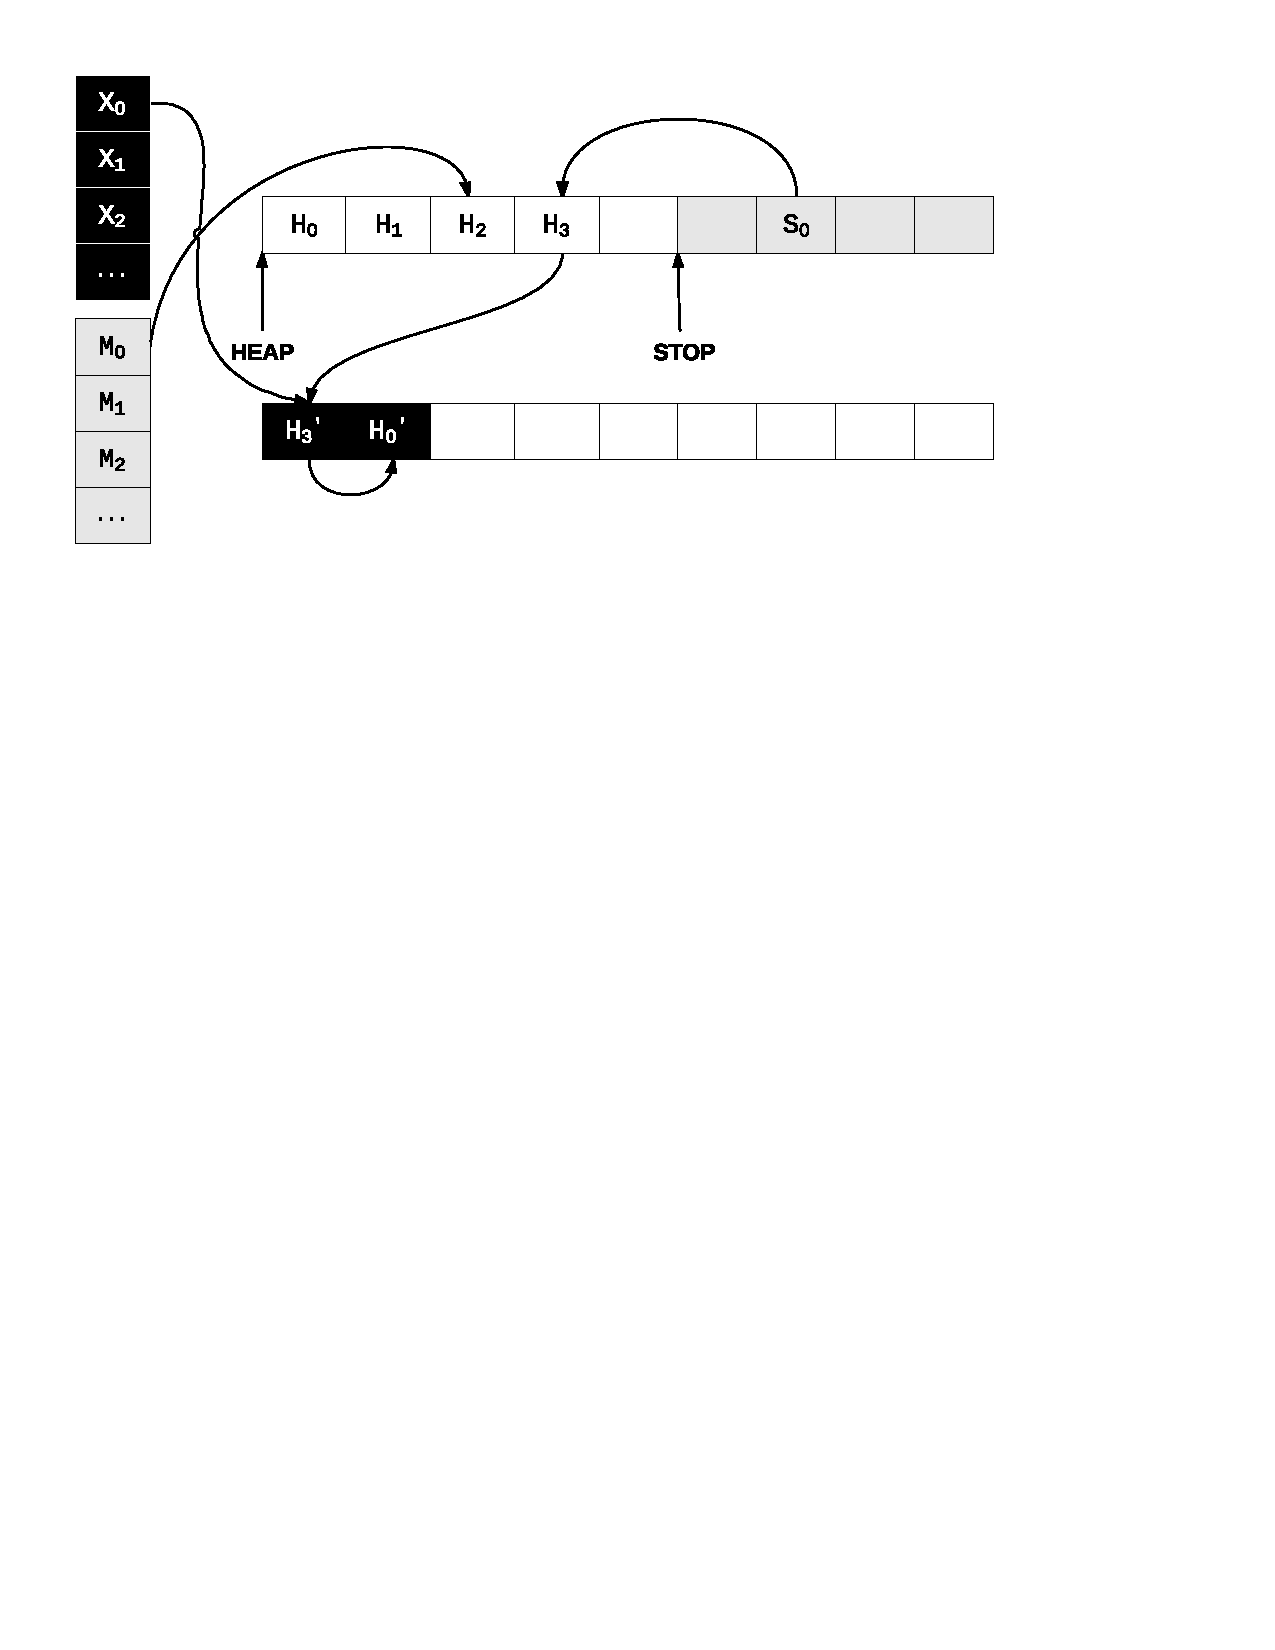
\includegraphics[scale=0.75, clip, trim=10mm 185mm 45mm 10mm]{gc_2}}
\caption{Przeniesienie wyrażeń mających źródło w rejestrach na nową stertę.}
\label{fig:gc2}
\end{figure}

Analogicznie, na nową stertę przeniesione zostało wyrażenie \textbf{H\textsubscript{2}}, do którego odnosiła się wiadomość \textbf{M\textsubscript{0}} (rys. \ref{fig:gc3}).

\begin{figure}[h]
\centerline{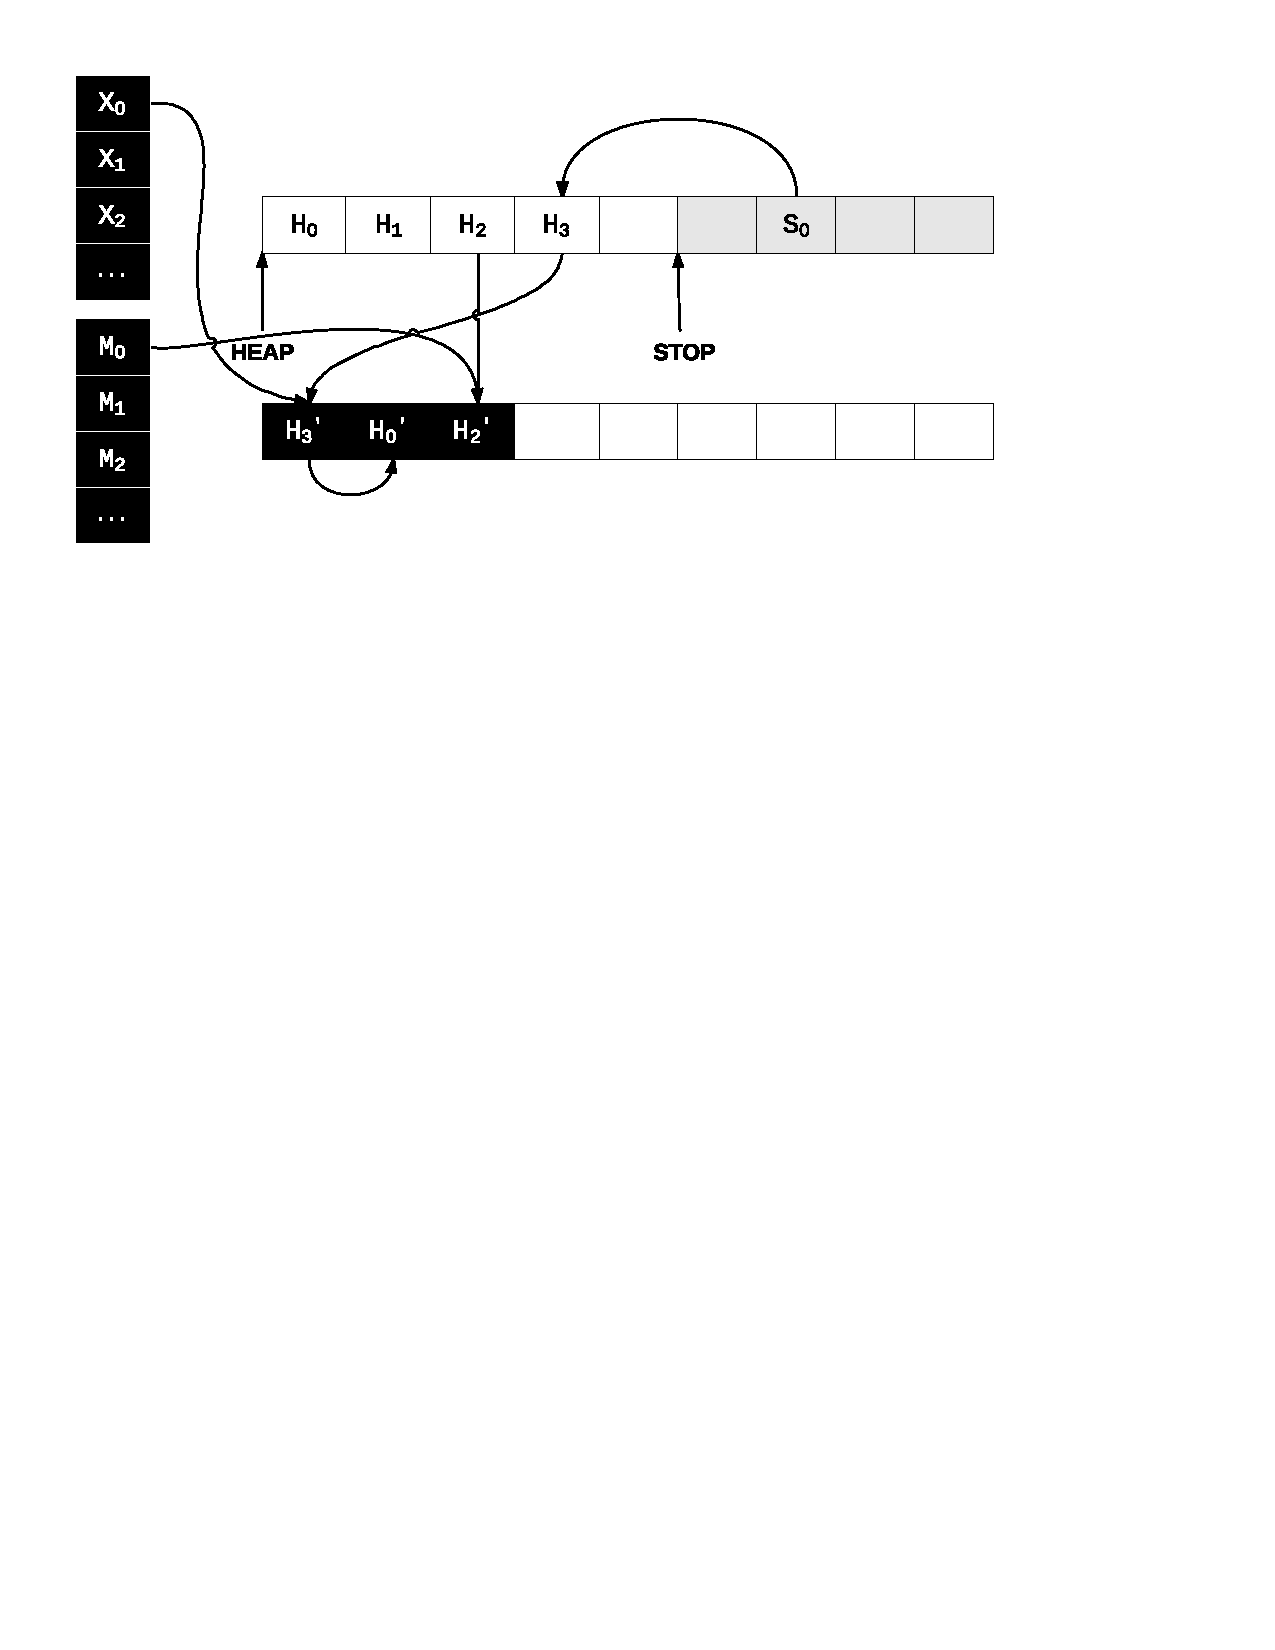
\includegraphics[scale=0.75, clip, trim=10mm 185mm 45mm 10mm]{gc_3}}
\caption{Przeniesienie wyrażeń mających źródło w kolejce wiadomości.}
\label{fig:gc3}
\end{figure}

Ostatnim analizowanym zbiorem szarym był stos procesu, w którym wyrażenie \textbf{S\textsubscript{0}} odnosiło się do, przeniesionego już wcześniej, wyrażenia \textbf{H\textsubscript{0}}. Dlatego też w tym kroku wystarczające było przepisanie referencji do kopii tego obiektu do wyrażenia na stosie (rys. \ref{fig:gc4}).

\begin{figure}[h]
\centerline{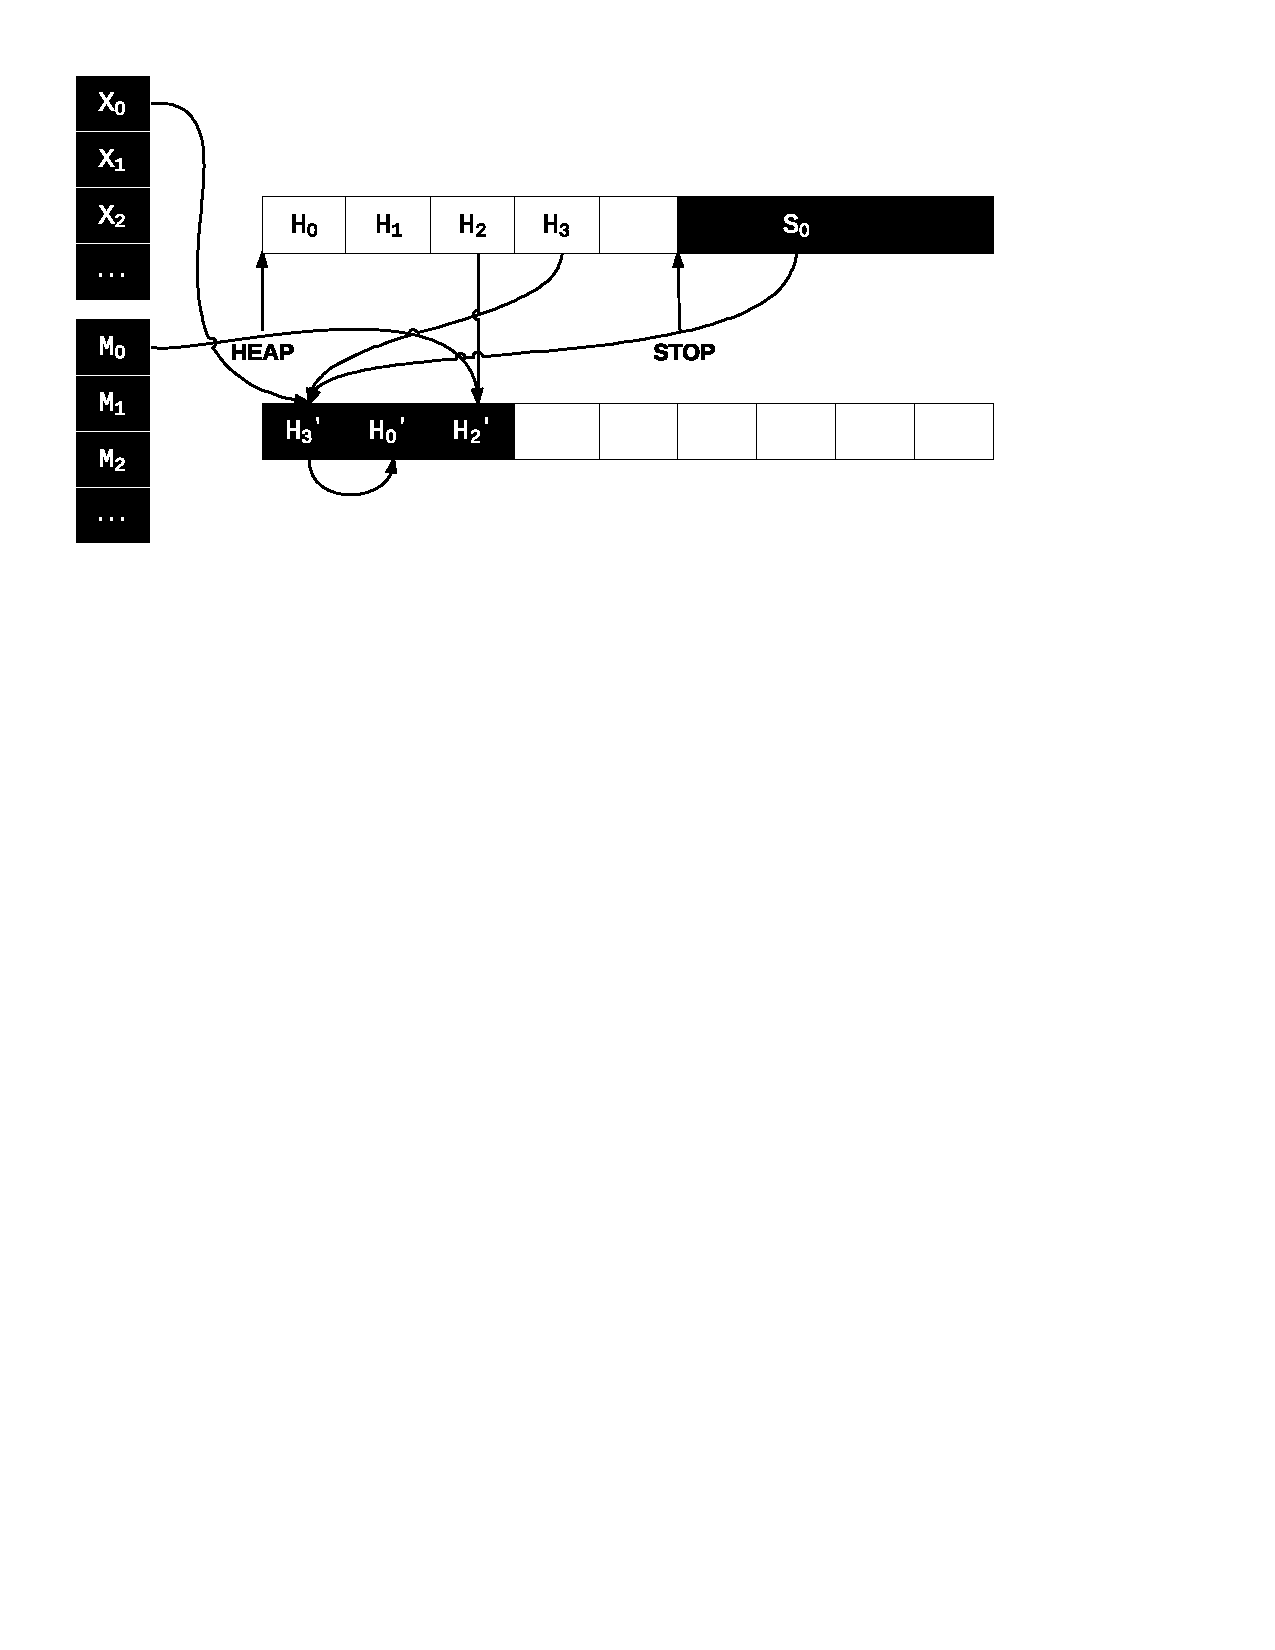
\includegraphics[scale=0.75, clip, trim=10mm 185mm 45mm 10mm]{gc_4}}
\caption{Podmiana wskaźnika do już przeniesionego wyrażenia.}
\label{fig:gc4}
\end{figure}

Przedostatnim krokiem działania algorytmu było skopiowanie stosu procesu, gdyż znajduje się on zawsze w tym samym bloku pamięci co sterta, a więc również zostaje usunięty w trakcie działania \emph{garbage collectora}.
Dokonano także przepisania odpowiednich wskaźników oznaczających początek sterty i stosu procesu (rys. \ref{fig:gc5}).

\begin{figure}[h]
\centerline{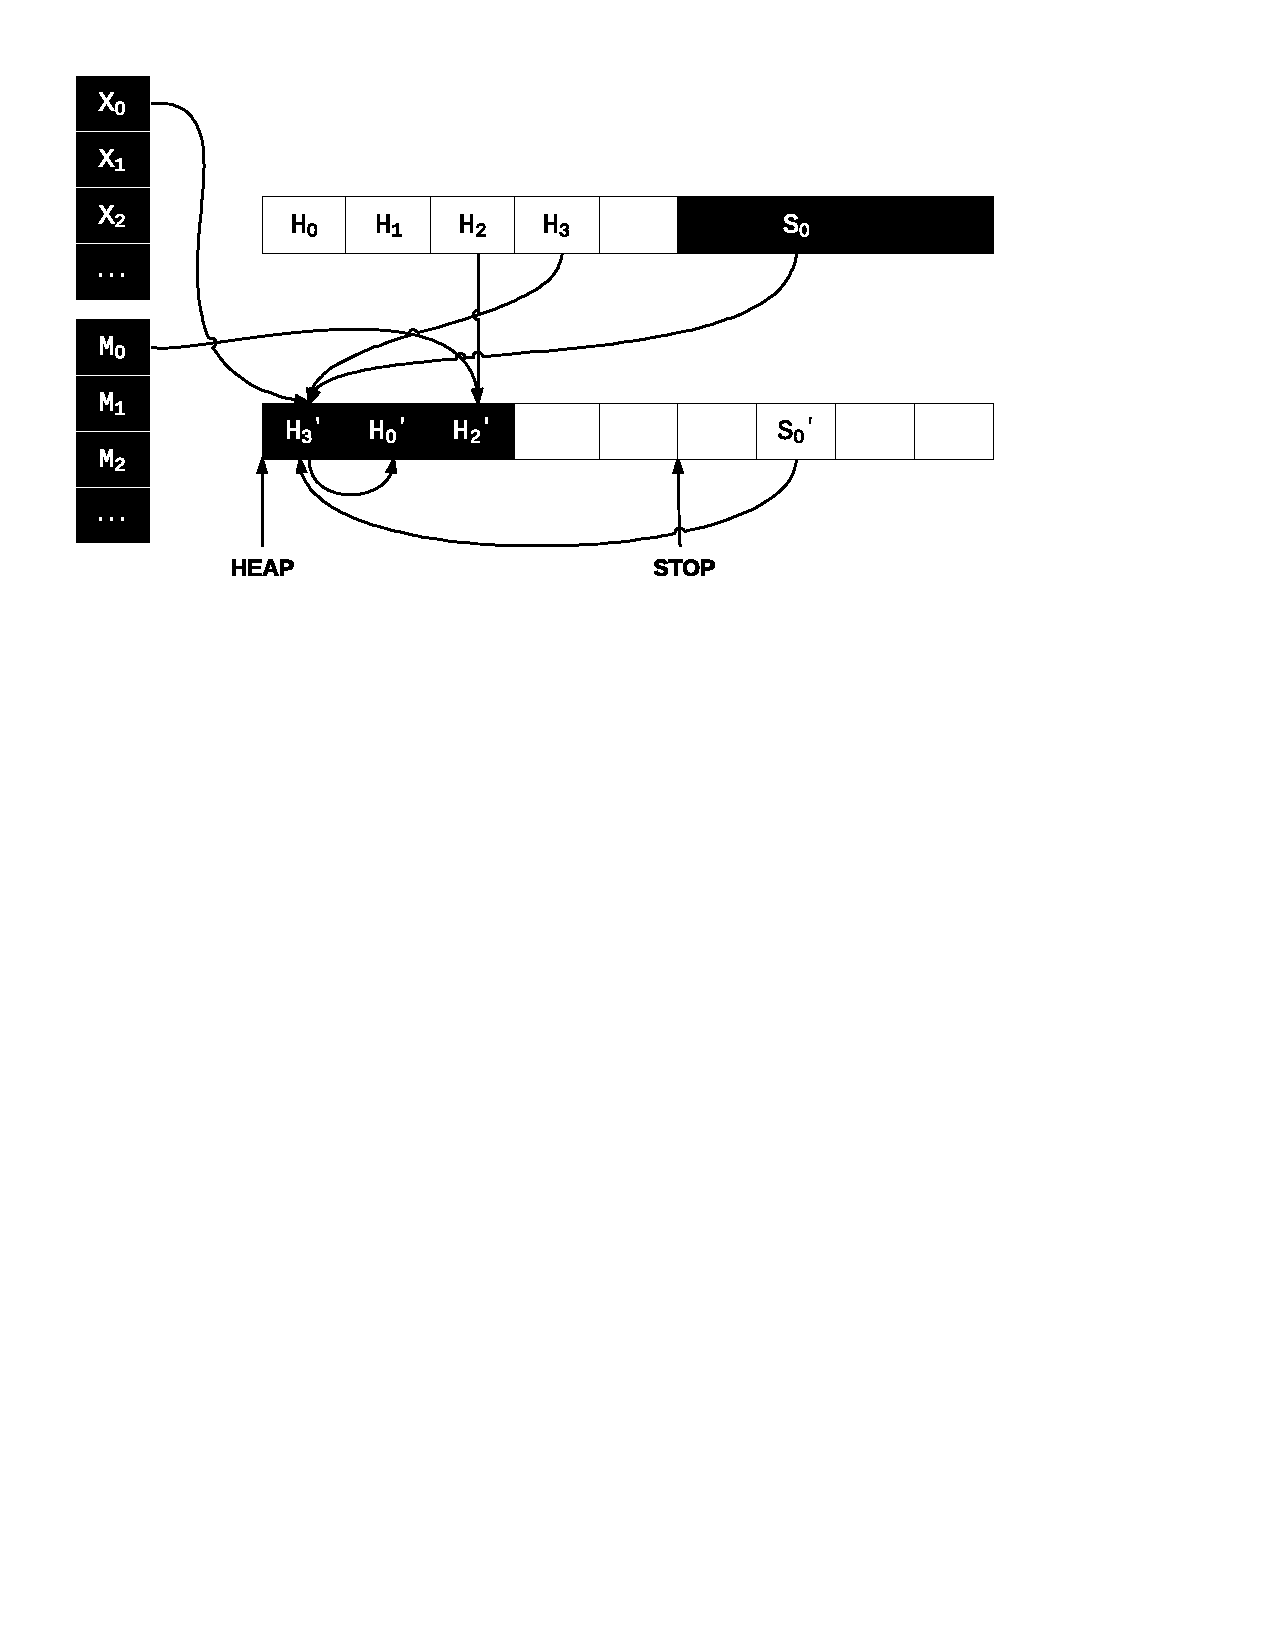
\includegraphics[scale=0.75, clip, trim=10mm 180mm 45mm 10mm]{gc_5}}
\caption{Kopiowanie stosu na nową stertę i przepisanie odpowiednich wskaźników.}
\label{fig:gc5}
\end{figure}

Końcowym krokiem działania algorytmu było zwolnienie dotychczas używanego bloku pamięci. Jak można zauważyć, na nowej stercie nie ma wyrażenia \textbf{H\textsubscript{1}}, które nie było już wykorzystywane w momencie uruchomienia algorytmu (rys. \ref{fig:gc6}).

\begin{figure}[h]
\centerline{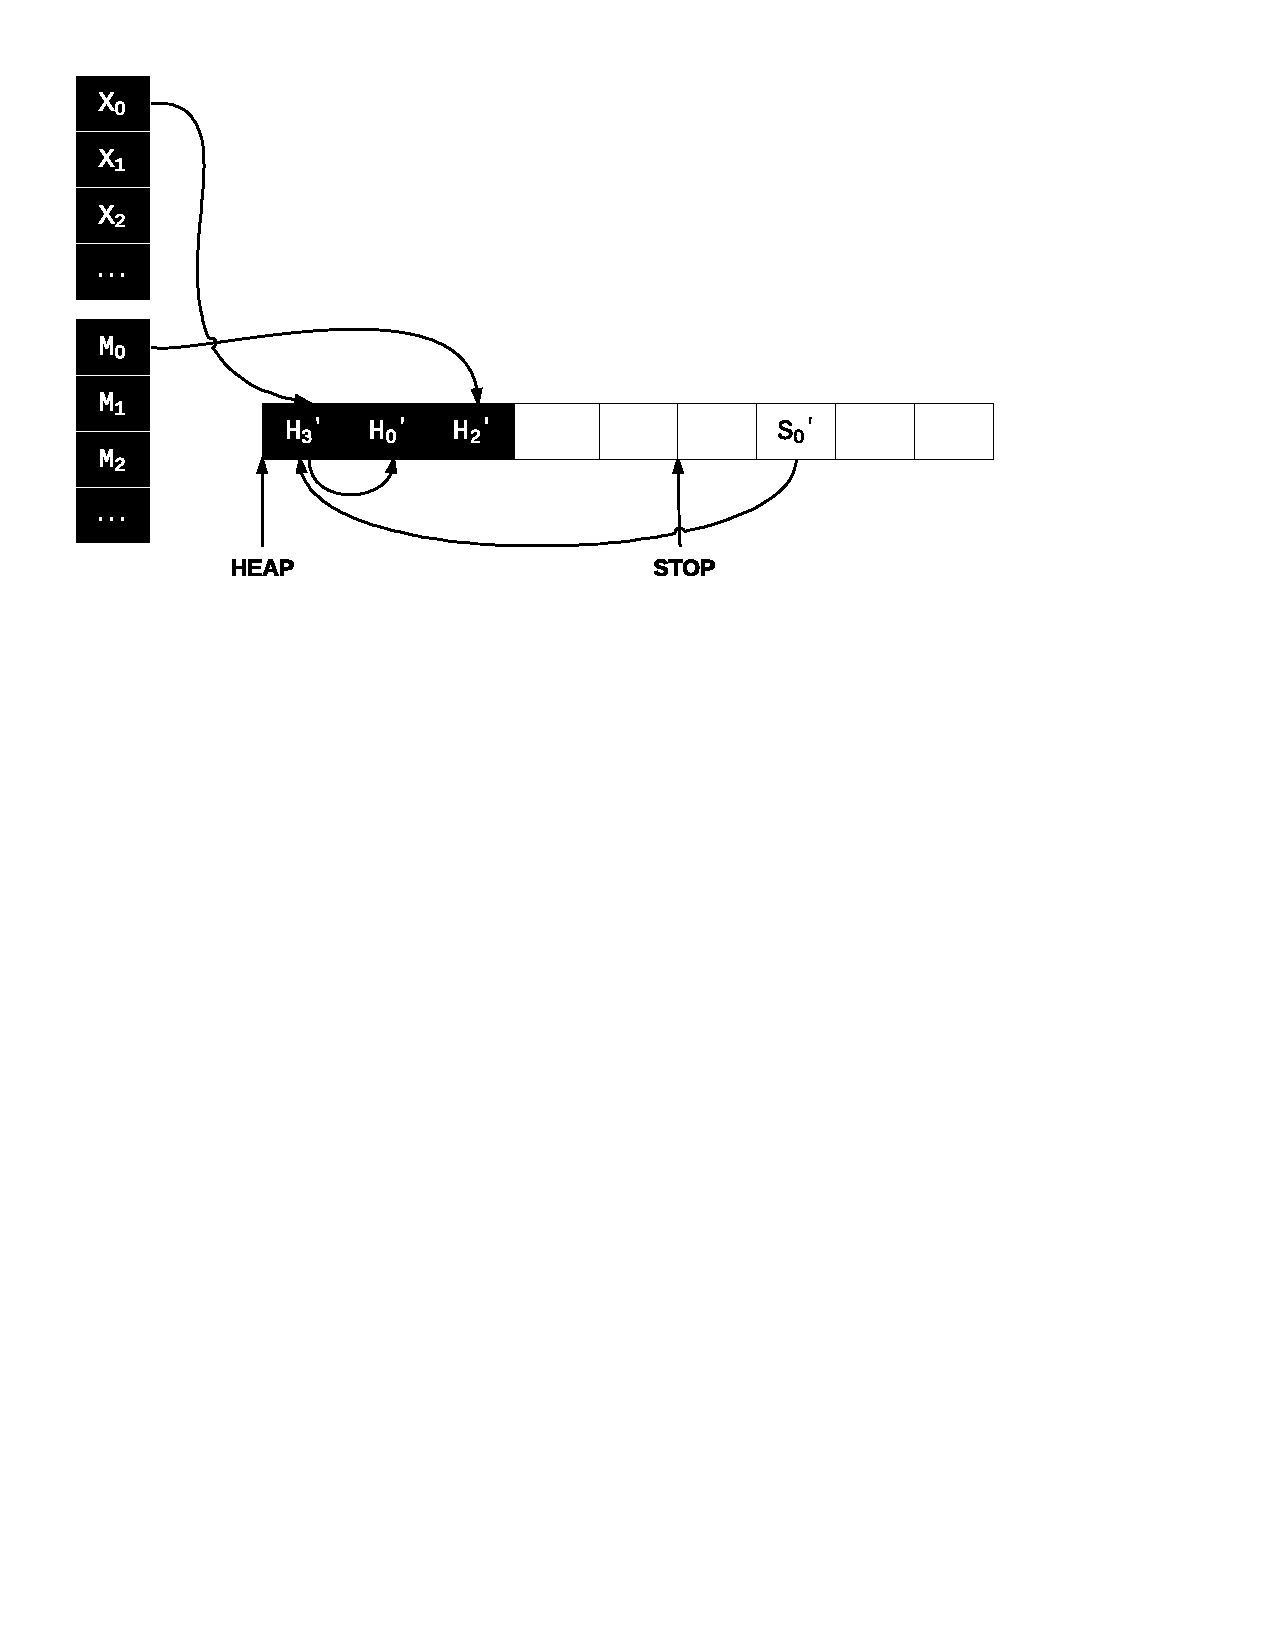
\includegraphics[scale=0.75, clip, trim=10mm 180mm 45mm 10mm]{gc_6}}
\caption{Zwolnienie pamięci zajmowanej przez starą stertę.}
\label{fig:gc6}
\end{figure}

Jeżeli dojdzie do sytuacji, w której po uruchomieniu \emph{garbage collectora} na stercie nie będzie odpowiedniej ilości miejsca dla nowych obiektów, dokonane zostanie rozszerzenie sterty. Polega ono na zaalokowaniu nowego obszaru pamięci, o kolejnym możliwym rozmiarze niż obecny i przeniesieniu stosu oraz wszystkich wyrażeń ze sterty.
W takiej sytuacji konieczne jest również przepisanie referencji obiektów do nowych miejsc w pamięci.
Po zakończeniu tego procesu źródłowa sterta jest zwalniania.

Analogiczną operację wykonuje się w sytuacji, gdy pamięć zajmowana przez nowe obiekty zajmuje co najwyżej pewnien ustalony rozmiar.
W maszynie wirtualnej został on ustalony na połowę rozmiaru starej sterty.
W takiej sytuacji sterta procesu jest zmniejszana do najbliższego wymaganemu rozmiarowi i, podobnie jak w przypadku rozszerzania sterty, zawartość sterty i stos przenoszone są do nowego bloku pamięci.

\subsection{Podejście generacyjne w maszynie BEAM}
\label{sub:gcGeneracje}

Maszyna BEAM w procesie odśmiecania korzysta dodatkowo z podejścia generacyjnego.
Opiera się ono na obserwacji, że większość utworzonych obiektów usuwana jest z pamięci stosunkowo wcześnie, a~obiekty które ,,przetrwały'' przynajmniej jedno uruchomienie \emph{garbage collectora} prawdopodobnie przetrwają i kolejne.
Prowadzi to do podziału obiektów na dwie generacje, którym przypisane są osobne sterty: ,,młodą'' i ,,starą''.
Pierwsza z nich zawiera niedawno utworzone obiekty, które nie zostały poddane jeszcze żadnemu procesowi odśmiecania.
Druga z kolei przechowuje obiekty, które zostały utworzone w pamięci przed przynajmniej jednym uruchomieniem \emph{garbage collectora}.
Odśmiecanie ,,starej'' sterty odbywa się z założenia zdecydowanie rzadziej niż jest to w przypadku obszaru pamięci z nowymi obiektami.
Częstość ta w maszynie wirtualnej BEAM jest parametrem konfigurowalnym przez zmienną środowiskową \texttt{ERL\_FULLSWEEP\_AFTER}, której wartość mówi co ile uruchomień \emph{garbage collectora} na ,,młodej'' generacji obiektów uruchomiony on zostanie również dla ,,starej'' generacji.
Im większa wartość, tym sam proces odśmiecenia trwa zdecydowanie krócej, proces wykorzystuje jednak więcej pamięci.

W maszynie wirtualnej zaimplementowanej w pracy nie została zaimplementowana ta optymalizacja algorytmu odśmiecania. 


%---------------------------------------------------------------------------
\section{Mechanizmy zarządzania czasem}
\label{sec:maszynaTimer}

Moduł opisany w niniejszym podrozdziale został zaimplementowany w pliku źródłowym \texttt{erl\_time.c}.

Język Erlang zapewnia dwie konstrukcje pozwalające na ustawienie przeterminowania po upływie zadanego czasu, po którym przez maszynę wirtualną zostanie wykonana pewna czynność:
\begin{itemize}
\item konstrukcja \texttt{receive ... after ... end} --- zawieszająca wykonywanie się procesu aż do momentu otrzymania wiadomości, kiedy to przeterminowanie zostaje usunięte z listy aktywnych lub do upłynięcia ustalonego czasu w milisekundach, kiedy proces wznawia działanie wykonując najpierw kod w bloku \texttt{after};
\item wywołanie funkcji wbudowanej \texttt{erlang:send\_after/3} --- kolejkującej wysłanie wiadomości do wskazanego procesu po upłynięciu zadanego czasu. Usunięcia tak utworzonego przeterminowania można dokonać poprzez wywołanie innej funkcji wbudowanej \texttt{erlang:cancel\_timer/1}.
\end{itemize}

Wymienione funkcjonalności związane z zarządzeniem przeterminowaniami zostały zaimplementowane w maszynie wirtualnej opisywanej w pracy.

Strukturą danych służącą do zapamiętania aktywnych przeterminowań jest koło czasowe, będące tablicą dwukierunkowych list przeterminowań, o określonej z góry długości. Sposób działania mechanizmu został zaprezentowany na rysunkach od \ref{fig:tiw1} do \ref{fig:tiw3}.

Na rysunku \ref{fig:tiw1} zaprezentowano wygląd struktury w momencie uruchomienia maszyny wirtualnej.
Koło czasowe ma tutaj 128 pól, a rozdzielczość każdego z nich to 1 milisekunda.
Wskaźnik, oznaczony na rysunkach czerwoną strzałką, zapamiętuje aktualne pole koła czasowego.
W momencie aktualizacji czasu wskaźnik ten jest przesuwany o odpowiednią liczbę pól, a w przypadku dojścia do końca tablicy ustawiany jest on ponownie na jej początku.
\begin{figure}[h]
\centerline{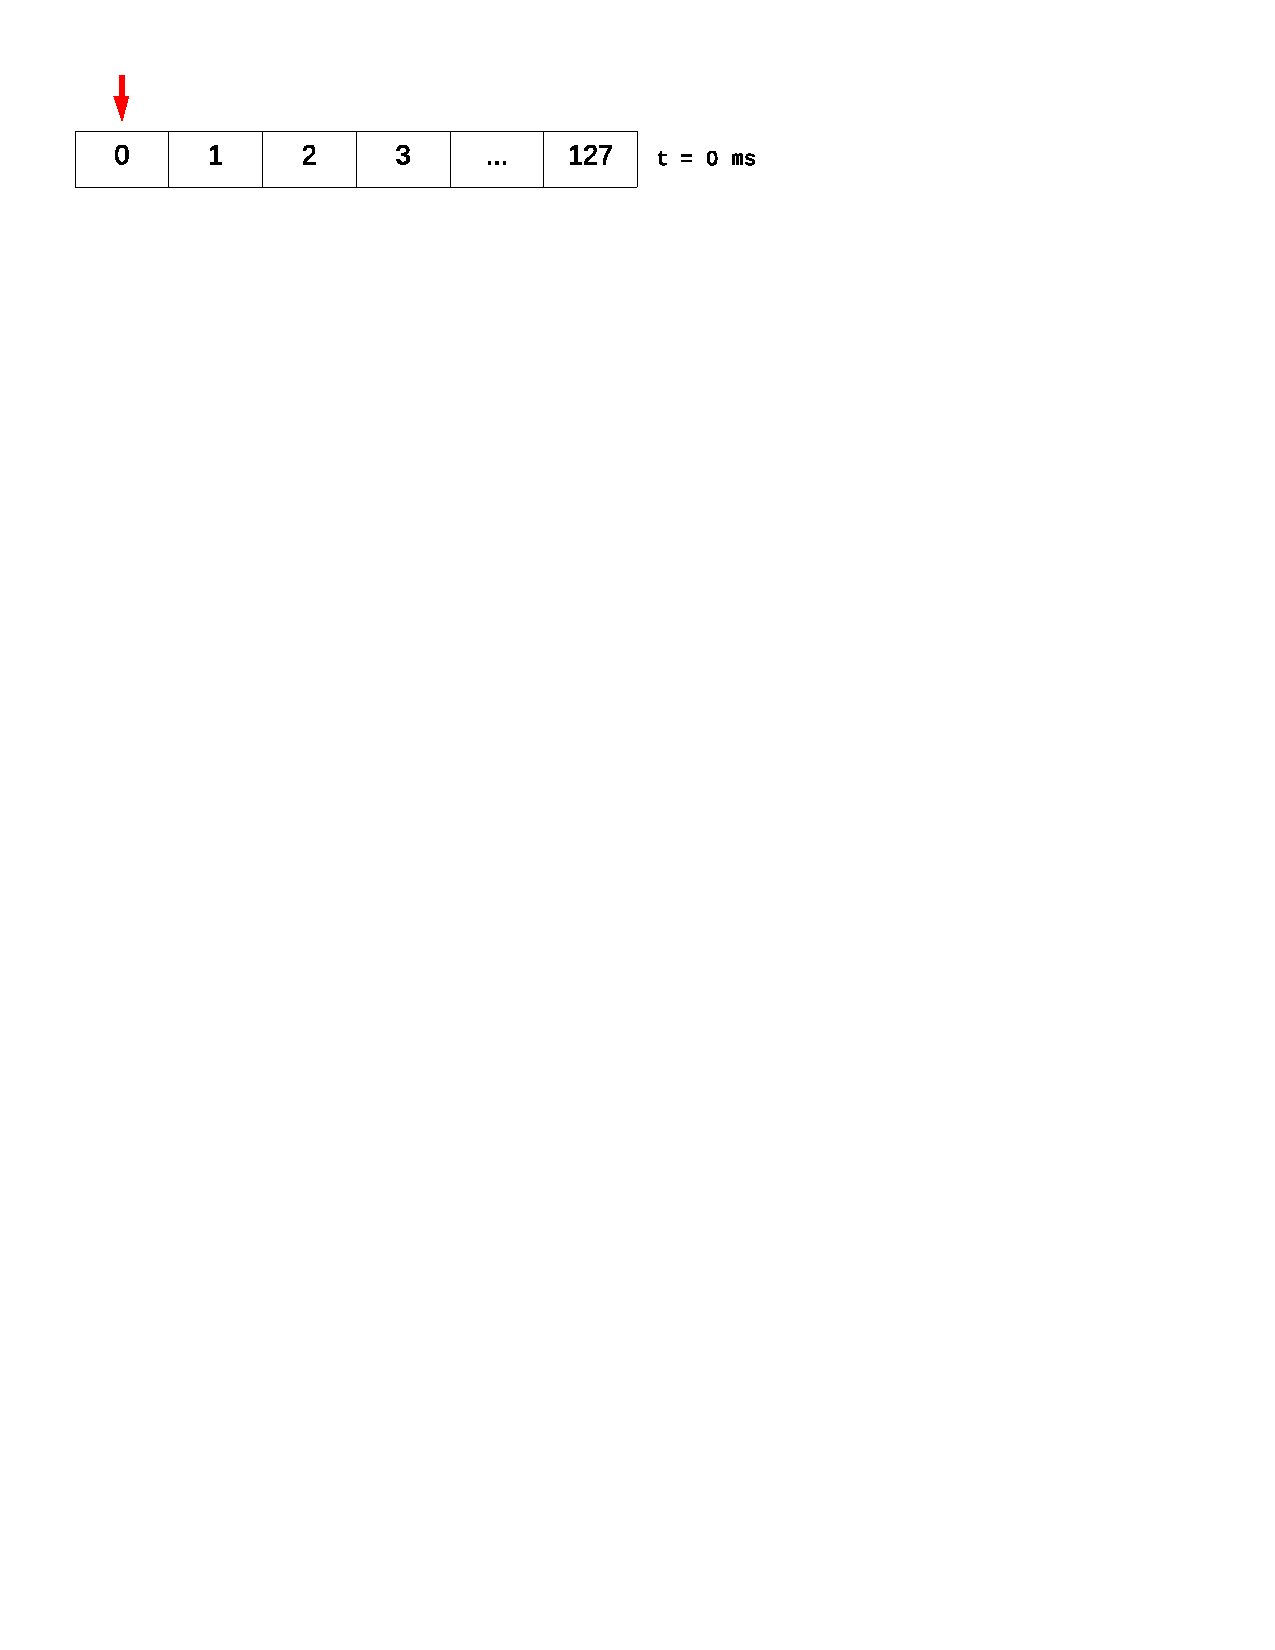
\includegraphics[scale=0.75, clip, trim=10mm 245mm 80mm 10mm]{tiw1}}
\caption{Stan koła czasowego w momencie uruchomienia systemu.}
\label{fig:tiw1}
\end{figure}

Na rys. \ref{fig:tiw2} zaprezentowano wygląd koła czasowego po upływie 2 milisekund od uruchomienia systemu.
W międzyczasie do koła czasowego dodano dwa przeterminowania:
\begin{itemize}
\item do zrealizowania za 1 milisekundę --- ponieważ aktualne pole w kole czasowym to 2, przeterminowanie zostało dodane na pozycji 3 i zostanie zrealizowane przy kolejnej aktualizacji czasu;
\item do zrealizowania za 257 milisekund --- realizacja przeterminowania może nastąpić dopiero po dwukrotnym przejściu wskaźnika przez całe koło czasowe (256 ms) i dojścia do pozycji nr 3~w~tablicy, dlatego w przypadku tego przeterminowania wartość licznika ustawiona została na 2.
\end{itemize}

\begin{figure}[h]
\centerline{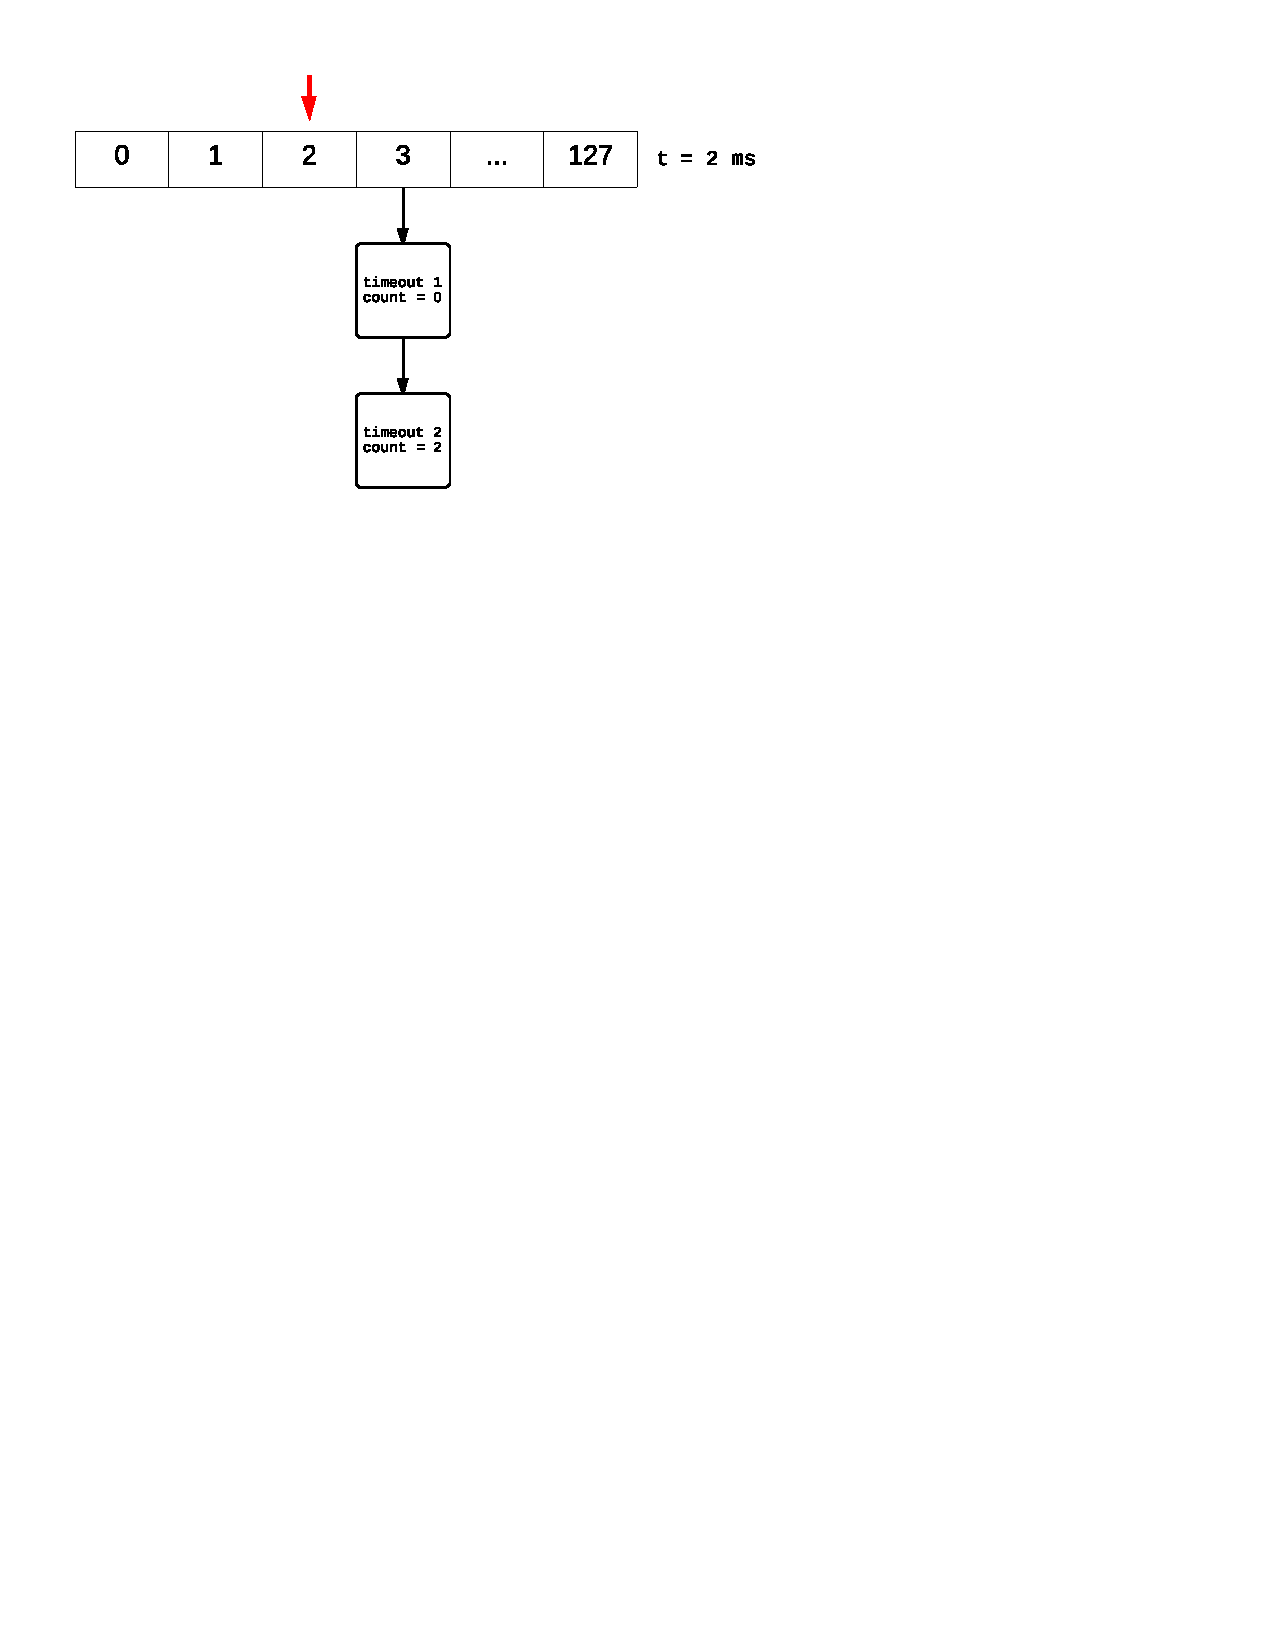
\includegraphics[scale=0.75, clip, trim=10mm 195mm 80mm 10mm]{tiw2}}
\caption{Koło czasowe z dodanymi dwoma przeterminowaniami.}
\label{fig:tiw2}
\end{figure}

Rysunek \ref{fig:tiw3} przedstawia stan koła czasowego w 259. milisekundzie.
Wskaźnik, oznaczony czerwoną strzałką, w porównaniu do stanu zaprezentowanego na poprzednim rysunku wykonał dwa pełne przejścia przez całą tablicę koła czasowego.
Każda aktualizacja czasu (przesunięcie wskaźnika) pociąga za sobą aktualizację przeterminowań na pozycjach mijanych przez wskaźnik.
Jeżeli licznik przeterminowania jest równy zeru oznacza to, że przeterminowanie powinno zostać zrealizowane i usunięte z listy na danej pozycji.
W przeciwnym wypadku, przeterminowanie przeznaczone jest do zrealizowania w którymś z kolejnych przejść wskaźnika przez daną pozycję koła czasowego. Dlatego też licznik danego przeterminowania zostaje zmniejszony o 1.

\begin{figure}[h]
\centerline{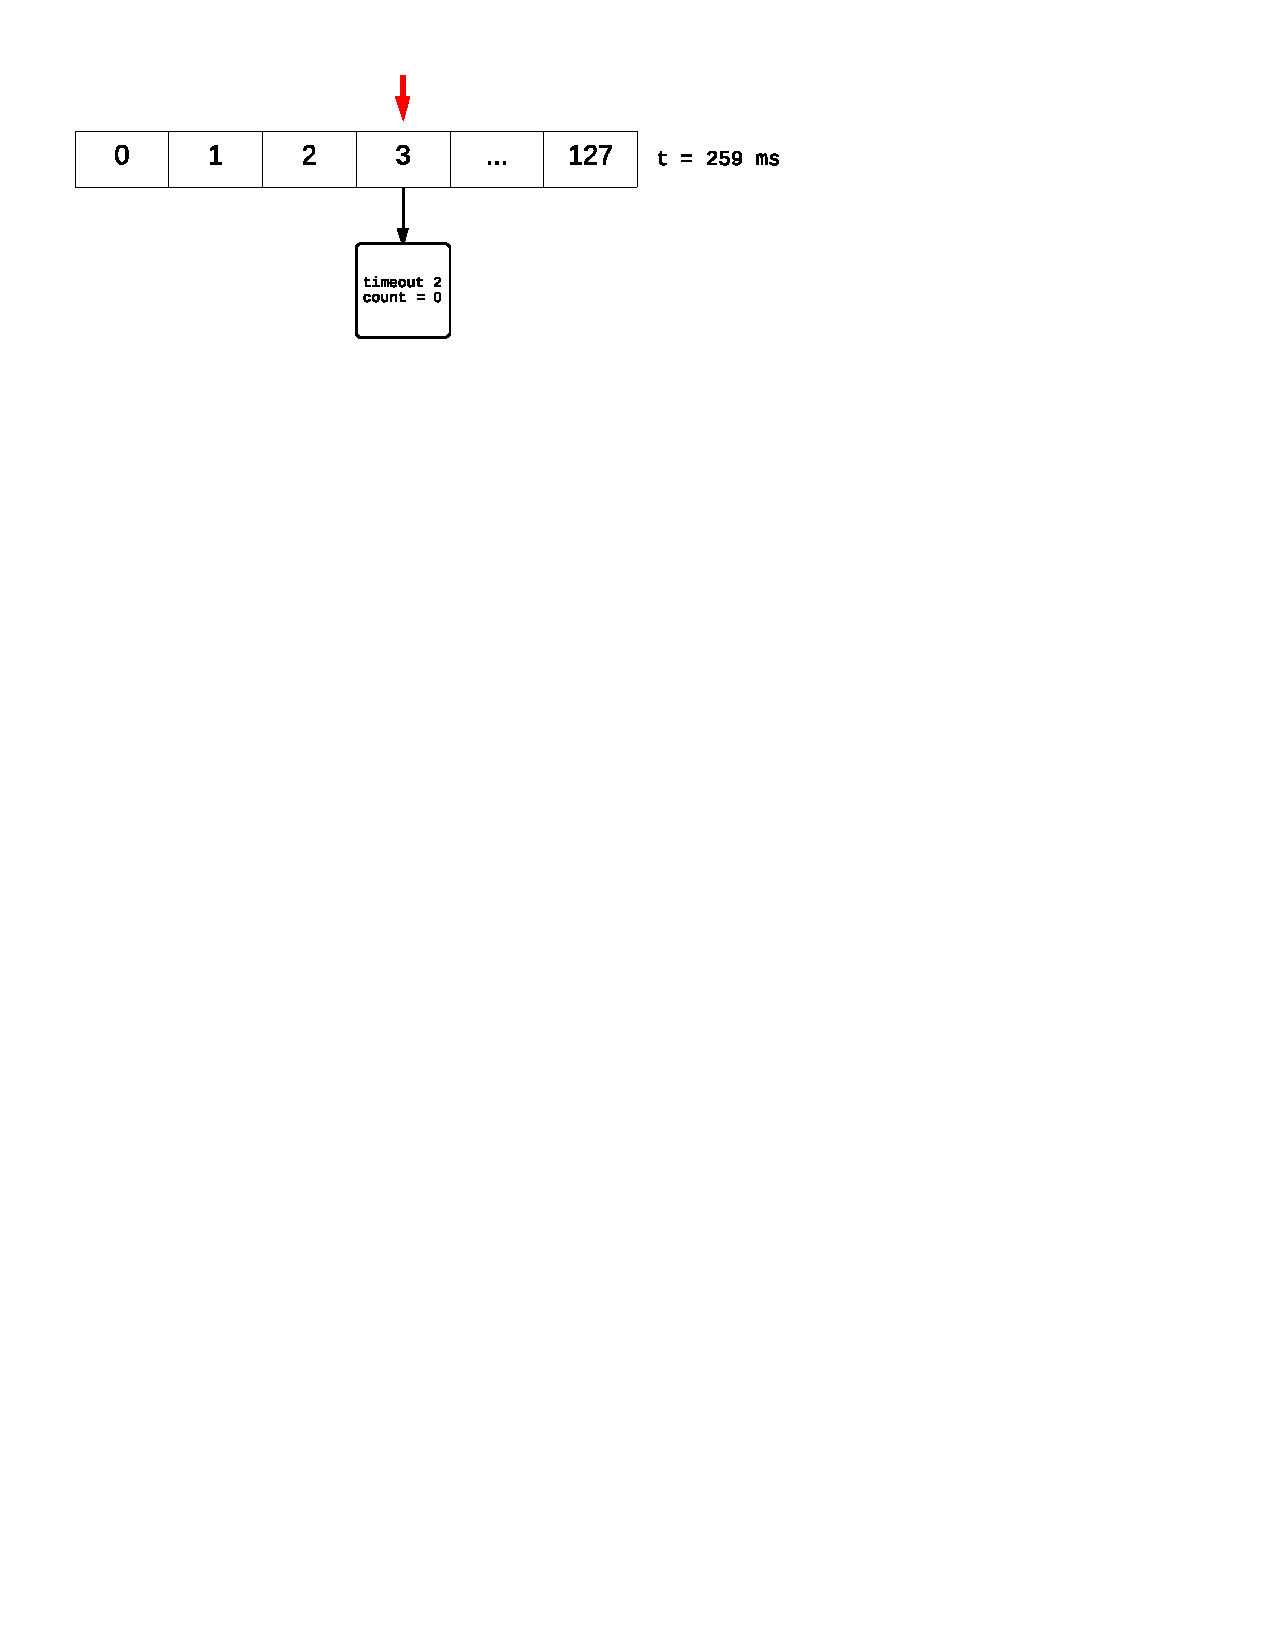
\includegraphics[scale=0.75, clip, trim=10mm 220mm 80mm 10mm]{tiw3}}
\caption{Koło czasowe z jednym przeterminowaniem, które zostanie zrealizowane przy kolejnej aktualizacji czasu.}
\label{fig:tiw3}
\end{figure}

Jedyną różnicą w budowie koła czasowa pomiędzy maszyną zaimplementowaną w pracy a maszyną BEAM jest jej rozmiar.
W maszynie BEAM składa się ona aż z 65536 pozycji.
Rozmiar ten, ze względu na ograniczony rozmiar dostępnej pamięci, w niniejszej maszynie został ograniczony do minimum.

Aspektem różniącym obie maszyny w działaniu mechanizmów zarządzania czasem jest również sposób aktualizacji czasu, a co za tym idzie częstość aktualizacji wskaźnika koła czasowego.
W maszynie wirtualnej BEAM wskaźnik aktualizowany jest na podstawie zegara systemowego pomiędzy wykonywaniem kolejnych procesów z kolejek, a także gdy nie ma w nich żadnych procesów do uruchomienia.
Z~kolei w zaimplementowanej maszynie wirtualnej rola aktualizacji czasu przejęta została przez fizyczny zegar aktualizowany taktowaniem o częstotliwości 1 kHz.
Zegar uruchamia przerwanie w mikrokontrolerze, a kod je obsługujący aktualizuje pozycję wskaźnika koła czasowego i aktualizuje jego stan wraz z~realizacją odpowiednich przeterminowań.
W idealnym przypadku więc pozycja wskaźnika będzie aktualizowana z częstotliwością równą rozdzielczości koła czasowego (co 1 milisekundę), jednak opóźnienia w obsłudze przerwania mogą prowadzić do rzadszej jego aktualizacji.

W niniejszej maszynie wirtualnej została zaimplementowana została także funkcja wbudowana \texttt{erlang:now/0}, różniąca się jednak działaniem od jej odpowiednika w maszynie BEAM tym, że zwraca czas jaki upłynął od momentu uruchomienia systemu, nie zaś od początku 1 stycznia 1970 r.
Czas pozyskiwany jest z, innego niż w przypadku aktualizacji czasu w kole czasowym, fizycznego zegara mikrokontrolera LPC1769, aktualizowanego taktowaniem o częstotliwości 1 MHz.

%---------------------------------------------------------------------------
\section{Podsumowanie różnic z maszyną BEAM}
\label{sec:maszynaPodsumowanie}

Na elementy, z których składa się maszyna wirtualna Erlanga można popatrzeć z punktu widzenia poszczególnych obszarów pamięci przez nią zajmowanych.

Do elementów tych należą:
\begin{itemize}
\item skompilowany kod wykonywalny modułów opisanych w niniejszym rozdziale;
\item tablice: atomów, eksportowanych funkcji, portów i procesów;
\item kolejki procesów i portów, na podstawie których \emph{scheduler} decyduje o wyborze kolejnego procesu do wykonania;
\item uruchomione procesy z informacjami kontrolnymi, kolejkami wiadomości i pamięcią do nich należącą;
\item załadowany kod pośredni modułów, który wykonywany jest w kontekście procesów;
\item globalna sterta, na której umieszczane są stałe wyrażenia pochodzące z plikami z modułów;
\item tablice ETS (\emph{Erlang Term Storage}) stanowiące w maszynie wirtualnej mutowalny obszar pamięci, w postaci bazy danych klucz-wartość;
\item sterta, na której przechowywane są dane typu binarnego, których długość wynosi przynajmniej 64 bajtów. Dane te mogą być współdzielone przez procesy, których liczba przechowywana jest przez licznik referencji, na którego podstawie \emph{garbage collector} zwalnia nieużywane już obszary pamięci.
\end{itemize}

Na rysunku \ref{fig:ertsmemory} zaprezentowany został powyższy podział, z uwzględnieniem elementów które posiada zarówno maszyna BEAM jak i maszyna zaimplementowana w pracy, które zostały oznaczone kolorem czarnym.
Kolorem niebieskim z kolei oznaczone zostały elementy, które nie zostały zaimplementowane w maszynie na system FreeRTOS.
Strzałki na diagramie przedstawiają fakt przechowywania wskaźników na elementy w jednym obszarze pamięci przed drugi.

\begin{figure}[h]
\centerline{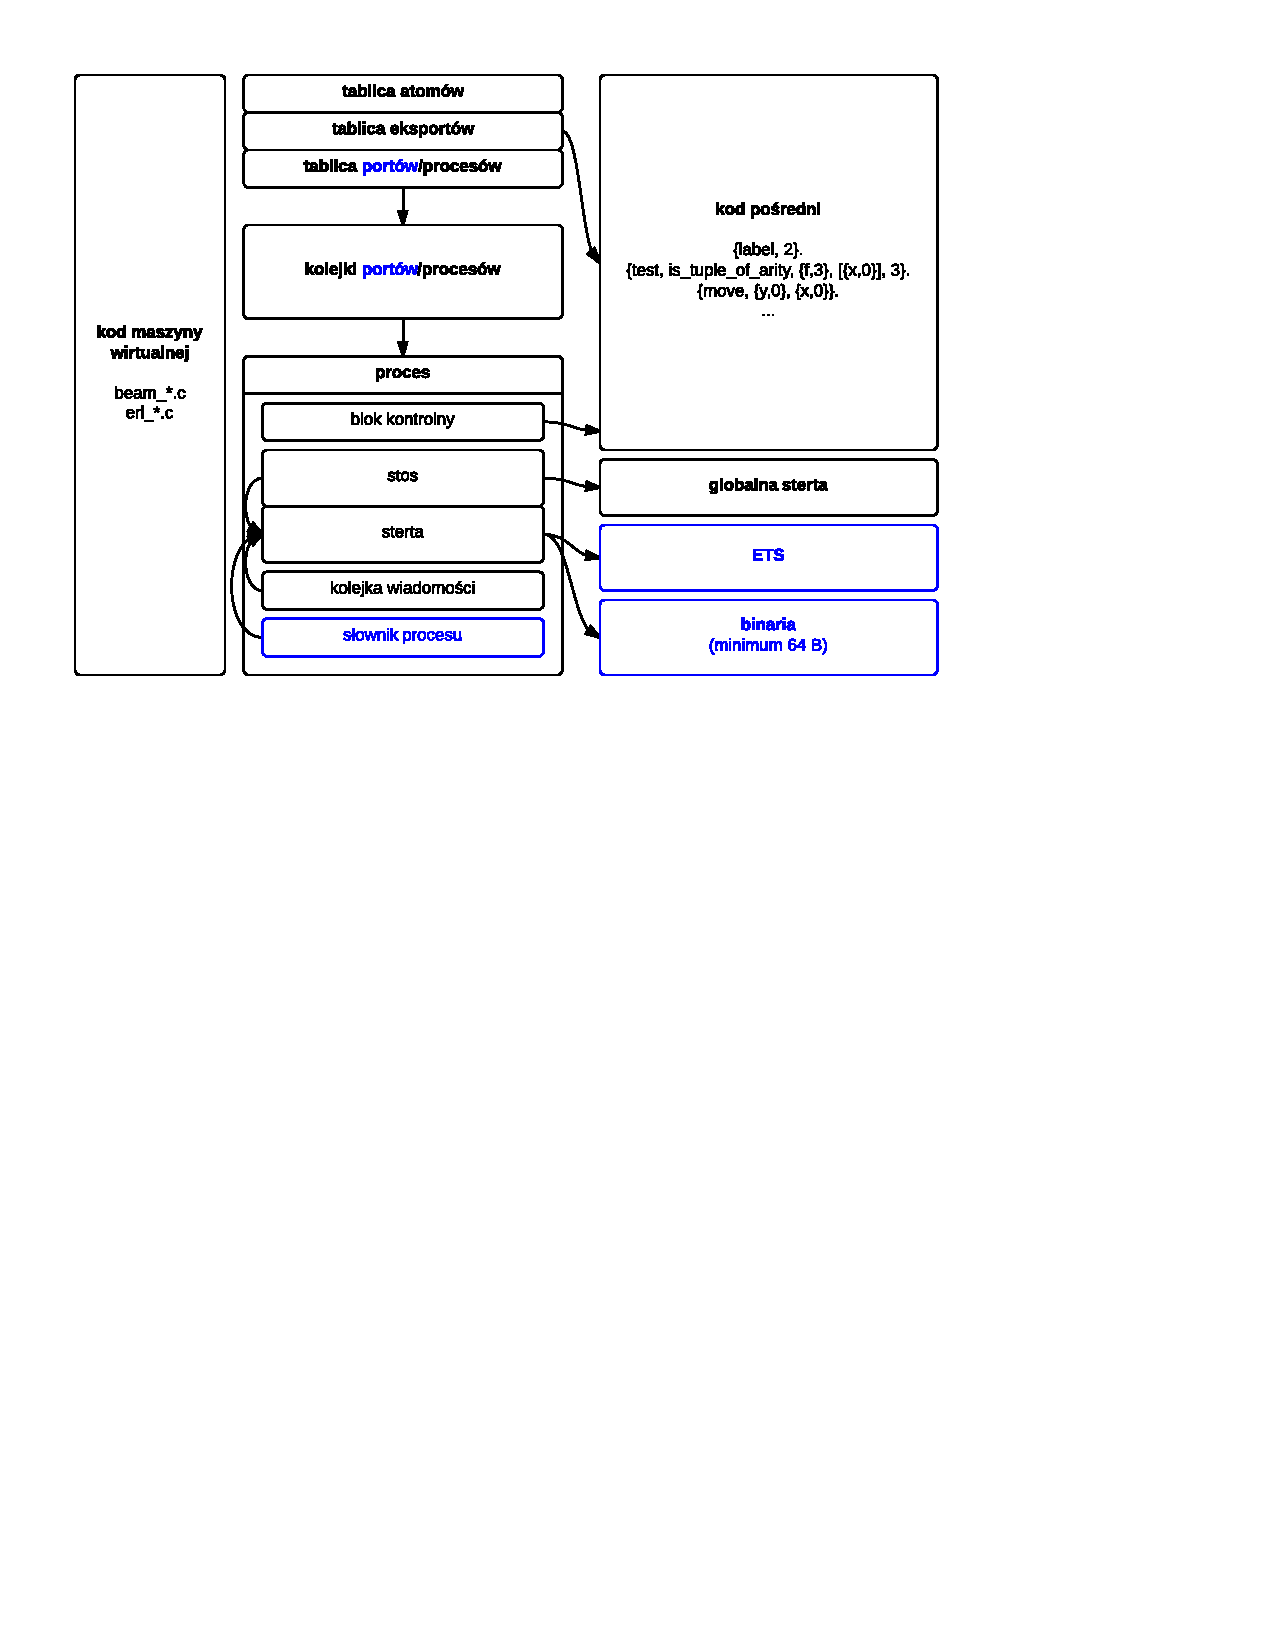
\includegraphics[scale=1, clip, trim=10mm 165mm 55mm 10mm]{erts_memory}}
\caption{Elementy maszyny wirtualnej Erlanga jako obszary pamięci.}
\label{fig:ertsmemory}
\end{figure}

Elementami, które nie zostały zaimplementowane w pracy są: tablice ETS oraz słownik procesu, których użycie nie jest konieczne do implementacji w pełni funkcjonalnych modułów w języku Erlang. Nie pozostały również zaimplementowane sterta binariów oraz tablice i kolejki portów, ze względu na niezaimplementowanie tych typów danych w maszynie.
%\chapter{Przykładowe aplikacje}
\label{cha:przyklady}

W niniejszym rozdziale pracy zaprezentowano przykładowe aplikacje zaimplementowane w języku Erlang i uruchomione na maszynie wirtualnej opisywanej w pracy. Platformą, na której uruchamiane były przykłady był mikrokontroler LPC1769 z procesorem ARM Cortex-M3 pod kontrolą mikrojądra FreeRTOS.

Wszystkie aplikacje zostały skompilowane przy użyciu narzędzia opisanego w dodatku \ref{cha:builder}. Kody źródłowe aplikacji zostały umieszczone na płycie CD dołączonej do pracy.

\section{Silnia}
\label{sec:przykladySilnia}

\subsection{Cel aplikacji}

Aplikacja miała na celu uruchomienie przykładowego sekwencyjnego programu zaimplementowanego w języku Erlang w dwóch wersjach: z rekurencją ogonową oraz bez tego typu rekurencji.

Rekurencja ogonowa charakteryzuje się tym, że wynik wywołania funkcji rekurencyjnej całkowicie zależy od wyniku rekurencyjnego wywołania funkcji.
Nie ma zatem konieczności powrotu do poprzedniego wywołania funkcji w celu ustalenia aktualnej wartości funkcji, a co za tym idzie zapisywania na stosie adresu powrotu i wyrażeń potrzebnych do wyliczenia zwracanego wyniku.
Kompilator Erlanga automatycznie wykrywa funkcje ogonowo-rekurencyjne i optymalizuje kod pośredni pod kątem użytego rozmiaru stosu (por. np. opis instrukcji \texttt{call} i \texttt{call\_only} na liście instrukcji kodu pośredniego na str. \pageref{sec:opsOps}).

Listingi \ref{lis:fac_facERL} oraz \ref{lis:fac_fac2ERL} przedstawiają kody źródłowe dwóch funkcjonalnie równoważnych sobie funkcji (\texttt{fac/1}) obliczających silnię liczby naturalnej.

\begin{figure}
\begin{multicols}{2}
\begin{lstlisting}[style=erlang, caption=Kod modułu \texttt{fac.erl}, label=lis:fac_facERL]
-module(fac).

-export([fac/1]).

fac(0) ->
    1;
fac(N) ->
    N*fac(N-1).



\end{lstlisting}

\columnbreak

\begin{lstlisting}[style=erlang, caption=Kod modułu \texttt{fac2.erl}, label=lis:fac_fac2ERL]
-module(fac2).

-export([fac/1]).

fac(N) ->
    fac(N, 1).

fac(0, Acc) ->
    Acc;
fac(N, Acc) ->
    fac(N-1, N*Acc).
\end{lstlisting}
\end{multicols}
\end{figure}

Funkcja z modułu \texttt{fac} wykorzystuje do tego celu tradycyjną rekurencję, uzależniając wynik zwrócony przez funkcję nie tylko od rekurencyjnego wywołania samej siebie, ale także od argumentu z jakim została wywołana. 

Funkcja zaimplementowana w module \texttt{fac2} wykorzystuje dodatkowy argument, tzw. akumulator, którego aktualna wartość przekazywana jest wraz z każdym kolejnym wywołaniem, a na samym końcu zwracana.
Dzięki zastosowaniu tego podejścia funkcja ta jest ogonowo-rekurencyjna, co pozwala na optymalizację użycia stosu przez kompilator Erlanga w kodzie pośrednim.

Celem eksperymentu było uruchomienie dwóch ww. funkcji obliczających silnię dla różnych wejściowych liczb naturalnych od 1 do 200. Pozwoliło to na sprawdzenie działania podstawowych elementów maszyny wirtualnej, m.in. interpretera kodu pośredniego, \emph{garbage collectora} czy arytmetyki dużych liczb (do zapisania wyniku $200!$ potrzebnych jest 156 bajtów).


\subsection{Uzyskane wyniki}

Silnia została obliczona dla wejściowych liczb: 1, 11 (wynik $11!$ jest ostatnim, jaki mieści się na 28 bitach i może zostać przechowany jako wyrażenie typu \textbf{SMALL}), 12 (wynik $12!$ jest ostatnim, jaki mieści się na 32 bitach i jest zarazem pierwszym, który do przechowania potrzebuje typu danych \textbf{BIGNUM}), 25, 50, 75, 100, 125, 150, 175 i 200. Dla wszystkich wartości wejściowych, dla obu modułów, uzyskano poprawne wartości silni.

Obliczenia zostały wykonane w kontekście procesu Erlanga, który był jedynym uruchomionym w~tym momencie na maszynie wirtualnej.

Czas wykonania mierzony był przy użyciu sprzętowego licznika wbudowanego w mikrokontroler, taktowanego zegarem o częstotliwości 1 MHz.

Rezultaty uzyskane w trakcie uruchomień zostały zaprezentowane na rysunku \ref{fig:facGraphs}.


Zgodnie z oczekiwaniami rozmiar sterty procesu w przypadku modułu \texttt{fac} rósł znacznie szybciej niż w przypadku modułu \texttt{fac2}, osiągając aż 610 słów maszynowych
w porównaniu do 90 słów w~przypadku funkcji ogonowo-rekurencyjnej dla obliczenia wyniku $200!$.
Na samo przechowanie stosu wywołań w pierwszym przypadku konieczne jest 400 słów maszynowych (200 liczb \textbf{SMALL} i 200 adresów powrotu).

Dużo większy rozmiar sterty dla pierwszego z modułów miał bezpośredni wpływ na dużo rzadsze uruchomienia \emph{garbage collectora}.
Ponieważ wyrażenia zajmujące znaczną część sterty (duże liczby) potrzebne były tylko w czasie jednego rekurencyjnego wywołania funkcji, przy każdym jego uruchomieniu zwalniana byłą dużą część pamięci. Większa część zaalokowanej sterty mogła zostać zatem później wykorzystana przez kolejne wywołania funkcji.

Z tego samego powodu w przypadku funkcji ogonowo-rekurencyjnej, \emph{garbage collectorowi} udało zwolnić się większą część pamięci (ok. 4500 słów maszynowych w porównaniu do ok. 3500 słów maszynowych).

Sam czas wykonywania kodu był nieco większy w przypadku modułu \texttt{fac} (2981 \textmugreek s w porównaniu do 2108 \textmugreek s), co wynika bezpośrednio z większej liczby instrukcji w kodzie pośrednim.
Czas spędzony na odśmiecaniu sterty procesu (ok. 43\% łącznego czasu wykonania programu w przypadku modułu \texttt{fac2} w porównaniu do ok. 21\% czasu dla drugiego modułu) miał jednak decydujący wpływ na łączny czas obliczenia silni, który okazał się wyraźnie większy dla modułu z funkcją ogonowo-rekurencyjną (4920 \textmugreek s w porównaniu do 3750 \textmugreek s).

Dla porównania, obie powyższe funkcje obliczające silnię z 200 na maszynie wirtualnej BEAM na komputerze z systemem operacyjnym MacOS X i procesorem Intel Core i7, wykonały się w ok. 1800 \textmugreek s.
Należy wspomnieć, że początkowy rozmiar sterty procesu został ustawiony na 12 słów maszynowych, tak jak jest to w przypadku maszyny implementowanej w pracy.


Różnicę można również zauważyć w liczbie wykonanych redukcji przez procesy, która jest nieco większa w przypadku wykonywania kodu z modułu \texttt{fac}.
Powodem tego jest fakt, że w całkowitą liczbę redukcji procesu wliczany jest czas uruchomienia \emph{garbage collectora}, ale tylko w przypadku gdy jest on uruchamiany przez instrukcje z rodziny \texttt{allocate} (opkody 12-15). Jeżeli \emph{garbage collector} uruchomiony zostanie w trakcie operacji arytmetycznej, redukcje nie są doliczane.
Ponieważ kod modułu \texttt{fac2} nie używa stosu, liczba redukcji przez niego wykonana pochodzi tylko i wyłącznie z wywołań funkcji.

\begin{figure}

\begin{multicols}{2}

\begin{gnuplot}[terminal=epslatex,terminaloptions=color,scale=0.7]
	set grid
	set title 'Pamięć zwolniona przez \emph{garbage collector}'
	set ylabel 'słowa maszynowe'
	set xlabel '$n$'
	set yr [0:5000]
	set size ratio 0.8
	plot 'facstats.csv' using 1:2 w p pt 7 ps 1 title 'fac:fac($n$)',\
			'facstats.csv' using 1:2 smooth csplines lt 3 lw 4 lc 1 notitle,\
			'fac2stats.csv' using 1:2 w p pt 7 ps 1 lc 3 title 'fac2:fac($n$)', \
			'fac2stats.csv' using 1:2 smooth csplines lt 3 lw 4 lc 3 notitle
\end{gnuplot}

\begin{gnuplot}[terminal=epslatex,terminaloptions=color,scale=0.7]
	set grid
	set title 'Uruchomienia \emph{garbage collectora}'
	set ylabel 'uruchomienia'
	set xlabel '$n$'
	set yr [0:180]
	set size ratio 0.8
	plot 'facstats.csv' using 1:3 w p pt 7 ps 1 title 'fac:fac($n$)',\
			'facstats.csv' using 1:3 smooth csplines lt 3 lw 4 lc 1 notitle,\
			'fac2stats.csv' using 1:3 w p pt 7 ps 1 lc 3 title 'fac:fac2($n$)', \
			'fac2stats.csv' using 1:3 smooth csplines lt 3 lw 4 lc 3 notitle
\end{gnuplot}

\begin{gnuplot}[terminal=epslatex,terminaloptions=color,scale=0.7]
	set grid
	set title 'Czas działania'
	set ylabel 'czas ($\mu s$)'
	set xlabel '$n$'
	set size ratio 0.8
	plot 'facstats.csv' using 1:5 w p pt 7 ps 1 title 'całkowity fac:fac($n$)',\
			'facstats.csv' using 1:5 smooth csplines lt 3 lw 4 lc 1 notitle,\
			'fac2stats.csv' using 1:5 w p pt 7 ps 1 lc 3 title 'całkowity fac:fac2($n$)', \
			'fac2stats.csv' using 1:5 smooth csplines lt 3 lw 4 lc 3 notitle,\
\end{gnuplot}


\begin{gnuplot}[terminal=epslatex,terminaloptions=color,scale=0.7]
	set grid
	set title 'Wykonane redukcje'
	set ylabel 'redukcje'
	set xlabel '$n$'
	set size ratio 0.8
	plot 'facstats.csv' using 1:4 w p pt 7 ps 1 title 'fac:fac($n$)',\
			'facstats.csv' using 1:4 smooth csplines lt 3 lw 4 lc 1 notitle,\
			'fac2stats.csv' using 1:4 w p pt 7 ps 1 lc 3 title 'fac:fac2($n$)', \
			'fac2stats.csv' using 1:4 smooth csplines lt 3 lw 4 lc 3 notitle
\end{gnuplot}


\begin{gnuplot}[terminal=epslatex,terminaloptions=color,scale=0.7]
	set grid
	set title 'Rozmiar sterty procesu'
	set ylabel 'słowa maszynowe'
	set xlabel '$n$'
	set size ratio 0.8
	plot 'facstats.csv' using 1:9 w p pt 7 ps 1 title 'fac:fac($n$)',\
			'facstats.csv' using 1:9 w steps lt 3 lw 4 lc 1 notitle,\
			'fac2stats.csv' using 1:9 w p pt 7 ps 1 lc 3 title 'fac:fac2($n$)', \
			'fac2stats.csv' using 1:9 w steps lt 3 lw 4 lc 3 notitle,\
\end{gnuplot}

\begin{gnuplot}[terminal=epslatex,terminaloptions=color,scale=0.7]
	set grid
	set title 'Czas działania'
	set ylabel 'czas ($\mu s$)'
	set xlabel '$n$'
	set yr [0:4000]
	set size ratio 0.8
	plot 'facstats.csv' using 1:7 w p pt 7 ps 1 title 'kod fac:fac($n$)',\
			'facstats.csv' using 1:7 smooth csplines lt 3 lw 4 lc 1 notitle,\
			'fac2stats.csv' using 1:7 w p pt 7 ps 1 lc 3 title 'kod fac:fac2($n$)', \
			'fac2stats.csv' using 1:7 smooth csplines lt 3 lw 4 lc 3 notitle,\
			'facstats.csv' using 1:6 w p pt 5 ps 1 lc 1 title 'GC fac:fac($n$)',\
			'facstats.csv' using 1:6 smooth csplines lt 3 lw 4 lc 1 notitle,\
			'fac2stats.csv' using 1:6 w p pt 5 ps 1 lc 3 title 'GC fac:fac2($n$)', \
			'fac2stats.csv' using 1:6 smooth csplines lt 3 lw 4 lc 3 notitle
\end{gnuplot}

\end{multicols}

\caption{Porównanie wyników uruchomienia modułów \texttt{fac} oraz \texttt{fac2} na implementowanej maszynie wirtualnej.}
\label{fig:facGraphs}

\end{figure}

\subsection{Wnioski}

Eksperymentalne uruchomienia funkcji obliczających silnię zwróciły poprawne wyniki, testując w~ten sposób arymetykę dużych liczb zaimplementowaną w maszynie wirtualnej.
Zmierzone czasy wykonania zarówno kodu jak i odśmiecania mogą stanowić punkt odniesienia przy przewidywania narzutu, jaki do aplikacji uruchamianej na mikrokontrolerze może wprowadzić maszyna wirtualna.
Na ich podstawie można wyciągnąć wniosek, że rekurencja ogonowa co prawda wykorzystuje zdecydowanie mniej pamięci, jednak przez dużą liczbę odśmieceń zajmuje więcej czasu. 

W momencie projektowania funkcji w Erlangu, która uruchamiana będzie na szybkim procesorze i~przy dostępnej dużej ilości pamięci, wybór pomiędzy rekurencją ogonową a tradycyjną nie ma większego znaczenia (o ile liczba wywołań nie jest bardzo duża, mogąca spowodować skończenie się dostępnej pamięci) i wybór implementacji powinien zostać podyktowany czytelnością kodu funkcji. Jednak w przypadku urządzeń wbudowanych, ze względu na bardzo ograniczone rozmiary zasobów, zawsze powinna być wybierana rekurencja ogonowa, która po optymalizacji kompilatora nie będzie używać stosu procesu w momencie rekurencyjnych wywołań funkcji.
Wydajność konkretnej aplikacji, poprzez zmniejszenie liczby uruchomień \emph{garbage collectora}, może zostać poprawiona przez wybór w pliku konfiguracyjnym początkowego rozmiaru sterty procesu, adekwatnego do jego logiki.


\section{Kontrola diod LED przez procesy}
\label{sec:przykladyDiody}

\subsection{Cel aplikacji}

Celem aplikacji było uruchomienie przykładowego programu korzystającego ze współbieżnych cech języka Erlang.
Aplikacja miała pozwolić na sprawdzenie działania takich funkcjonalności maszyny wirtualnej jak:
przesyłania i odbierania wiadomości między procesami, propagacji zakończenia działania procesu (\emph{link}) czy mechanizmów zarządzania czasem (przeterminowania i wysyłania wiadomości do innych procesów z opóźnieniem).

W tym celu zaimplementowano dwa moduły: \texttt{led\_sup} i \texttt{led\_drv}, których zadaniem była kontrola diod LED, przez zaimplementowane funkcje kontrolujące GPIO, w dwóch kolorach: czerwonym i~zielonym.
W systemie uruchomiony był jeden proces implementujący logikę pierwszego z modułów oraz osiem procesów - drugiego z nich.
Każdy z procesów \texttt{led\_drv} kontrolował stan jednej zielonej diody - zapalał lub gasił ją po otrzymaniu wiadomości z procesu \texttt{led\_sup}. Proces ten, w odstępie sekundowym, wysyłał do trzech losowych procesów wiadomość o zmianie stanu diody. Dodatkowo, w logice procesu ustawione zostało przeterminowanie, efektem którego było zakończenie się działania procesu w~sytuacji, gdy żadna wiadomość kontrolująca stan diody nie przyszła do skrzynki odbiorczej procesu w~odstępie 2 sekund.

Stan systemu wizualizowało dodatkowo osiem czerwonych diod, które były zgaszone w momencie gdy procesy kontrolujące odpowiadający im diody zielony były uruchomione i zapalone w przeciwnym wypadku.
Pojedynczy proces był procesem nadzorczym (\emph{supervisor}), którego zadaniem było ponowne uruchamianie kończących się procesów kontrolujących diody zielone. W tym celu, proces ten musiał działać jako proces przechwytujący wyjścia procesów z nim powiązanych jako wiadomości (co w języku Erlang realizowane jest poprzez ustawienie flagi procesu \texttt{trap\_exit} na \texttt{true}).
Dla czytelniejszej prezentacji stanu systemu w przykładzie, proces kontrolujący diodę zieloną restartowany był dopiero po upływie przynajmniej dwóch sekund po otrzymaniu wiadomości o zakończeniu się jego poprzednika.

Zależności między procesami uruchomionymi w ramach przykładowej aplikacji zostały zaprezentowane na rysunku \ref{fig:exampleledprocesses}. Fizyczna realizacja podłączeń diod, sterowanych stanem niskim, do mikrokontrolera wykorzystanego w przykładzie przedstawiona została na rysunku \ref{fig:exampleled}. Na obu rysunkach diody zostały oznaczone tymi samymi symbolami.

\begin{figure}[h]
\centerline{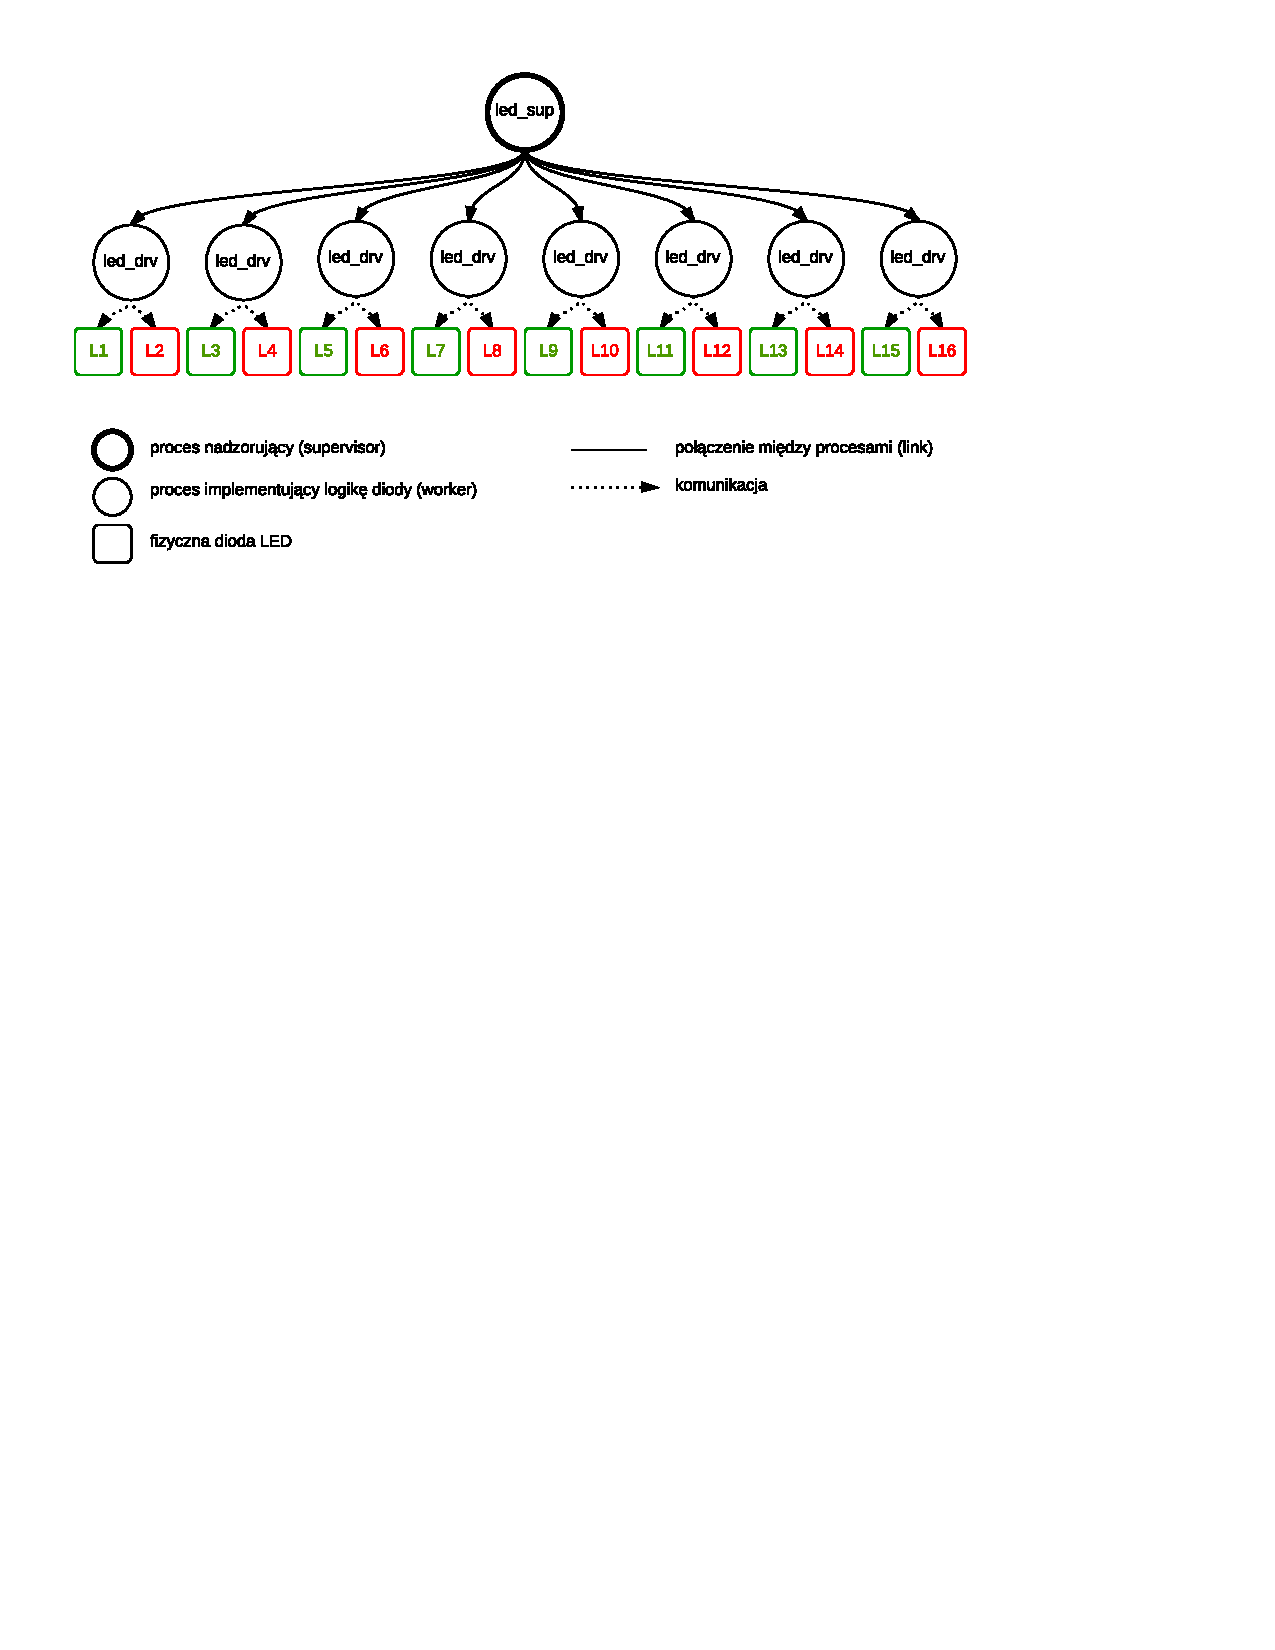
\includegraphics[scale=1, clip, trim=0 180mm 50mm 0]{example_led_processes}}
\caption{Struktura procesów w aplikacji i kontrolowanych przez nie diod}
\label{fig:exampleledprocesses}
\end{figure}

\begin{figure}[h]
\centerline{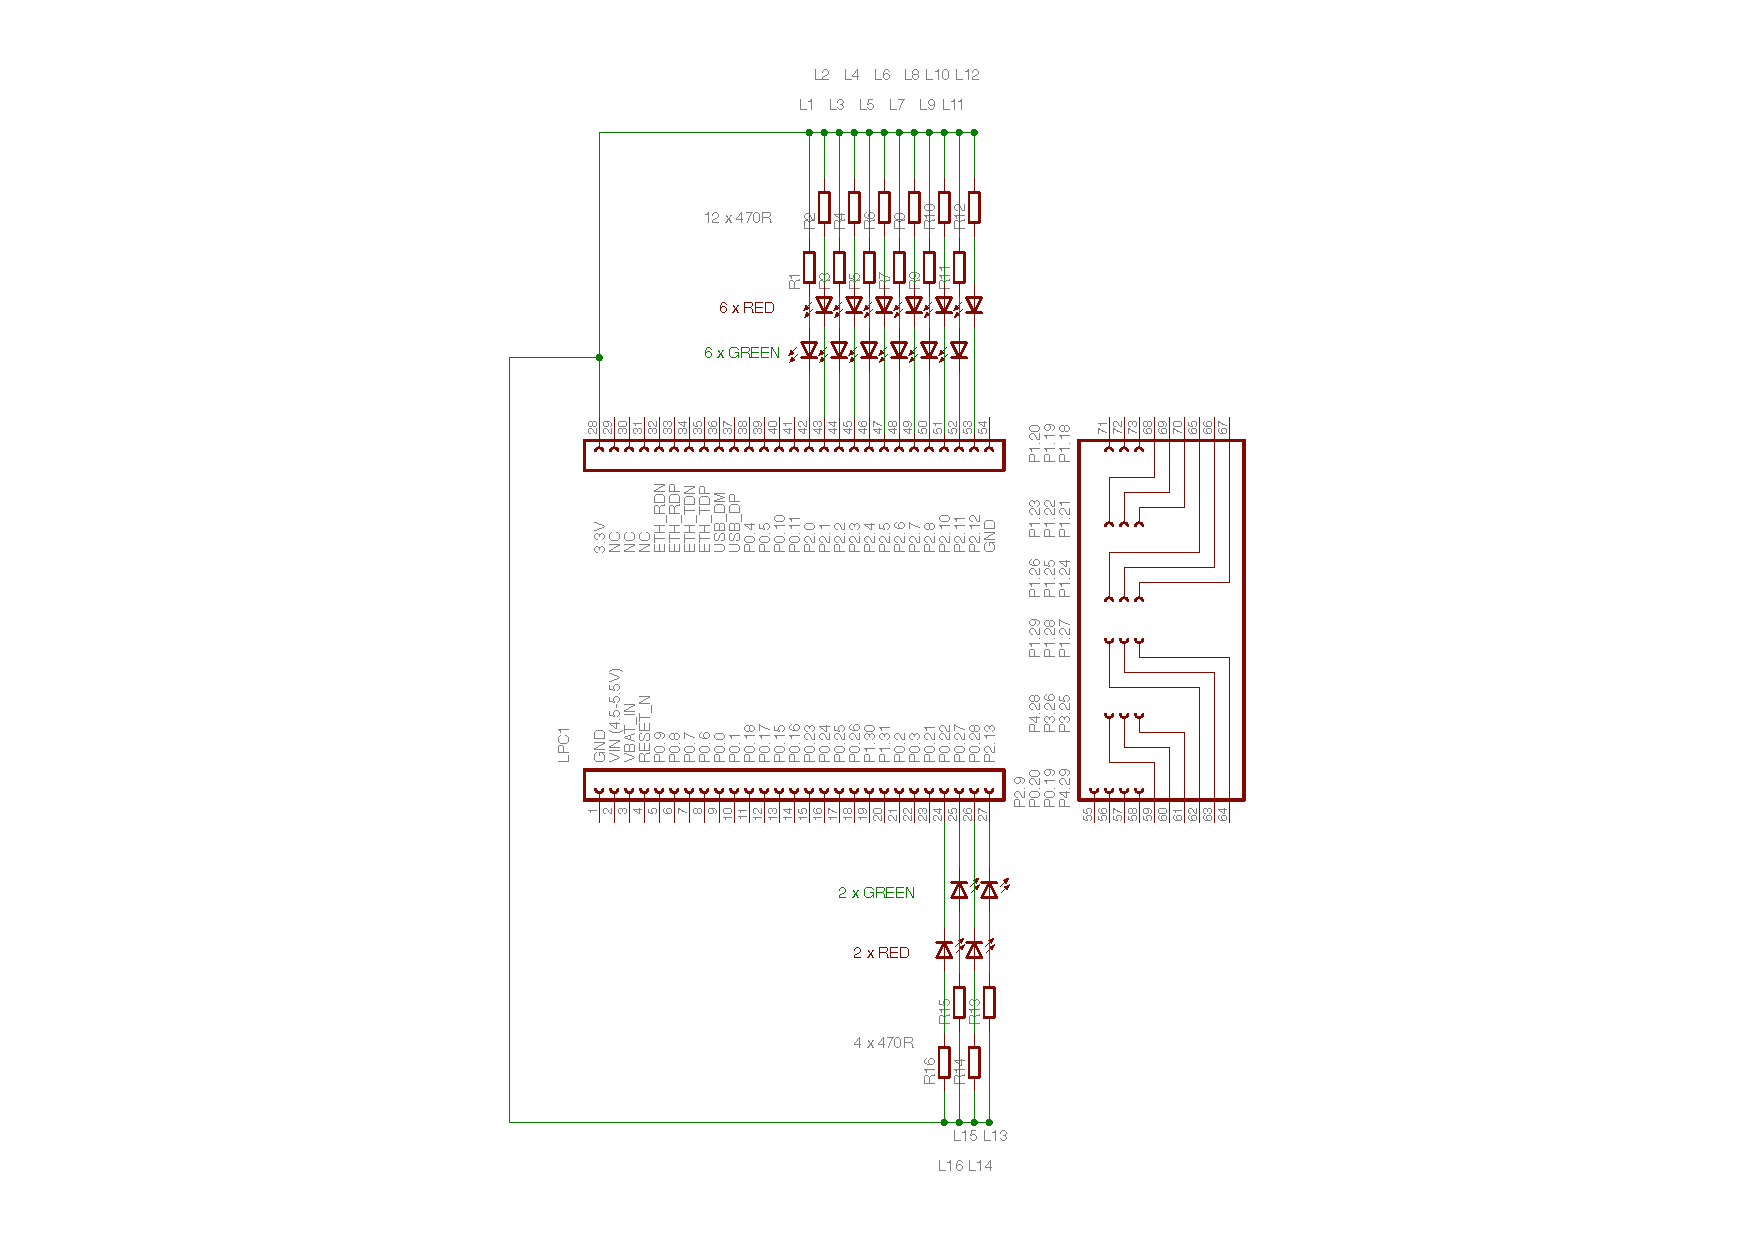
\includegraphics[scale=1, clip, trim=0 0 0 0]{example_led}}
\caption{Schemat podłączenia diod LED do płytki prototypowej z mikrokontrolerem LPC1769}
\label{fig:exampleled}
\end{figure}


\subsection{Uzyskane wyniki}

\subsection{Wnioski}


\section{Sterownik RFM73}
\label{sec:przykladyRfm}

\subsection{Cel aplikacji}

Celem aplikacji było zaimplementowanie biblioteki sterownika do modułu radiowego RFM73 \cite{RFM73}, produkowanego przez firmę Hope Microelectronics.
Ten tani układ (koszt jednej sztuki to ok. 10 PLN) pozwala na komunikację bezprzewodową w paśmie 2,4 GHz z szybkością dochodzącą do 2 Mbps. Warstwa sprzętowa zapewnia możliwość wysłania pakietu składającego się z maksymalnie 32 bajtów.
Odpowiedzialność za implementację protokołu pozwalającego na wysyłanie dłuższych pakietów należy już jednak do programisty.

Moduł komunikuje się ze światem zewnętrznym dzięki wbudowanemu w niego mikrokontrolerowi, za pomocą interfejsu szeregowego SPI (\emph{Serial Peripheral Interface}). Sam układ zapewnia także sprawdzanie poprawności pakietu za pomocą sumy kontrolnej, prosty mechanizm retransmisji czy adresowania urządzeń w sieci.

Typowymi zastosowaniami modułu mogą być takie urządzenia jak np:
\begin{itemize}
\item urządzenia zdalnego sterowania;
\item sensory przesyłające dane pomiarowe;
\item urządzenia peryferyjne do komputerów osobistych.
\end{itemize}

Implementowana aplikacja miała pozwolić na przykładowe obsłużenie urządzenia peryferyjnego w~języku Erlang, w tym wypadku za pomocą zaimplementowanych funkcji wbudowanych obsługujących interfejs SPI.
Udostępnione funkcje wyprowadzeń z modułu RFM73 pozwoliły również na zaimplementowanie biblioteki w ten sposób, by możliwe było przetestowanie tłumaczenia przerwań zewnętrznych zgłaszanych do mikrokontrolera na wiadomości wysyłane do procesów.

Fizyczna realizacja podłączeń układu do płytki uruchomieniowej z mikrokontrolerem LPC1769, na którym uruchamiany był niniejszy przykład została zaprezentowana na rysunku \ref{fig:examplerfm}.

\begin{figure}[h]
\centerline{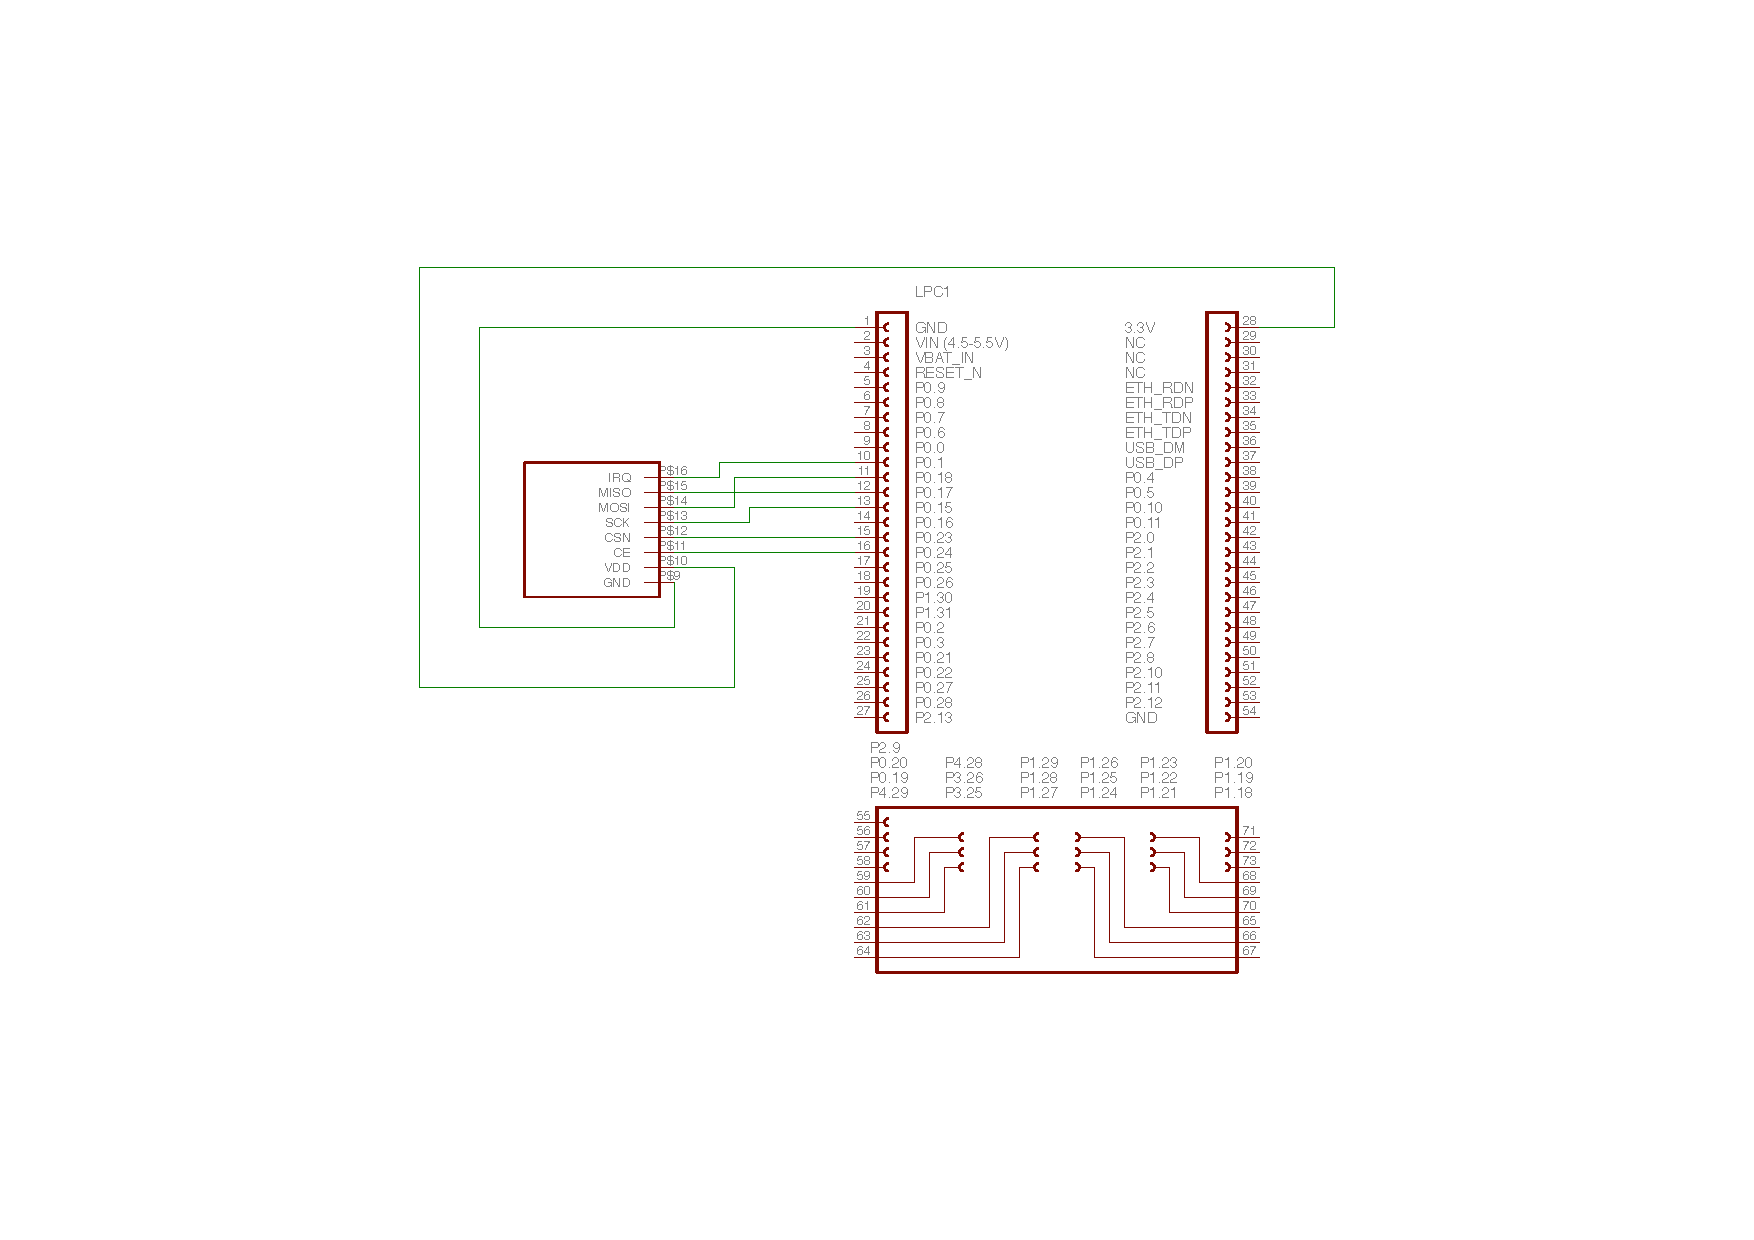
\includegraphics[scale=1, clip, trim=0 30mm 0 30mm]{example_rfm}}
\caption{Schemat podłączenia modułu RFM73 do płytki prototypowej z mikrokontrolerem LPC1769}
\label{fig:examplerfm}
\end{figure}


\subsection{Uzyskane wyniki}

Implementowany sterownik miał zapewnić abstrakcję modułu RFM73 z poziomu aplikacji napisanej w~języku Erlang z interfejsem pozwalającym na łatwe wysyłanie i odbieranie wiadomości drogą radiową. W celu przetestowania działania modułu, wysłano zestaw krótkich pakietów do innego urządzenia z podłączonym modułem tego samego typu. Program odbierający wiadomości po drugiej stronie odpowiadał wiadomościami o tej samej treści, dzięki czemu zweryfikowano poprawność danych przesyłanych w~dwie strony.


\subsection{Wnioski}

Zaimplementowana biblioteka może być również podstawą do implementacji protokołu \emph{Distributed Erlang}, dzięki któremu możliwy byłby do uruchomienia klaster urządzeń komunikujących się za pomocą modułu RFM73.
%\chapter{Podsumowanie}
\label{cha:podsumowanie}



\appendix
%\chapter{Zawartość dołączonej płyty CD}
\label{cha:cd}
%---------------------------------------------------------------------------

Na dołączonej do niniejszej pracy płycie CD znajdują się następujące pliki:

\begin{itemize}

\item plik \texttt{praca.pdf} zawierający treść niniejszej pracy w formacie Portable Document Format;
\item katalog \texttt{tex} zawierający źródło niniejszej pracy w  \LaTeX;
\item katalog \texttt{src} zawierający kod źródłowy implementacji maszyny wirtualnej opisanej w pracy;
\item katalog \texttt{prezentacja} zawierający źródła i plik wyjściowy w formacie PDF prezentacji do niniejszej pracy;
\item katalog \texttt{examples} zawierający przykładowe aplikacje opisane w rozdziale \ref{cha:przyklady};
\item katalog \texttt{builder} zawierający narzędzie do budowy aplikacji do uruchomienia na maszynie wirtualnej, opisane w dodatku \ref{cha:builder};
\item katalog \texttt{FreeRTOS\_Library} zawierający kod źródłowy mikrojądra FreeRTOS w wersji 8.0.1;
\item katalog \texttt{CMSISv1p30\_LPC17xx} zawierający zestaw nagłówków pomocnicznych dla mikrokontrolera LPC1769.

\end{itemize}
%\chapter{Kompilator aplikacji}
\label{cha:builder}
%---------------------------------------------------------------------------

Dodatek zawiera opis działania pomocnicznego narzędzia utworzonego dla potrzeb pracy, służącego do przygotowywania skompilowanych modułów Erlanga do włączenia w maszynę wirtualną uruchamianą pod systemem FreeRTOS.


\section{Opis aplikacji}
\label{sec:builderOpis}
%---------------------------------------------------------------------------
Maszyna wirtualna Erlanga dla systemu FreeRTOS implementowana w ramach pracy, na obecnym poziomie zaawansowania wymaga wkompilowania bajtkodu modułu w maszynę wirtualną.
Kod źródłowy maszyny oczekuje specjalnie przygotowanego pliku \texttt{modules.h}, który zawiera kod modułów a~także moduł, funkcję i argumenty, które zaczną być wykonywane w momencie startu maszyny.
Cały kod źródłowy maszyny wirtualnej może zostać następnie skompilowany wraz z mikrojądrem FreeRTOS, za pomocą platformy NXP LPCXpresso \cite{LPCXpresso}, przeznaczonej do rozwijania i programowania aplikacji na mikrokontrolery serii LPC.

Niniejsze narzędzie służy właśnie do generowania pliku \texttt{modules.h}, którego skopiowanie do katalogu z kodem źródłowym maszyny wirtualnej spowoduje włączenie wybranych modułów do maszyny wirtualnej.
Oprócz tego, przed wygenerowaniem właściwego pliku wyjściowego, narzędzie dokonuje rozpakowania fragmentów kodu modułu, które zostały spakowane algorytmem \textbf{zlib}.
Funkcjonalność ta została uwzględniona ze względu na fakt, że moduł ładujący kod w maszynie opisywanej w pracy nie posiada zaimplementowanego algorytmu dekompresji tego formatu.

\section{Kompilacja narzędzia}
\label{sec:builderKompilacja}
%---------------------------------------------------------------------------

Narzędzie zostało zaimplementowane w języku Erlang, dlatego też do jego kompilacji wymagany jest kompilator Erlanga. Narzędziem budującym projekt jest \texttt{rebar}, który również jest wymagany.

Aby skompilować aplikację, wystarczy użyć komendy \texttt{make} w głównym katalogu aplikacji. Plikiem wyjściowym będzie plik wykonywalny \texttt{freertos}, stanowiący samodzielną aplikację. Możliwe zatem jest skopiowanie go do wygodnego w użyciu folderu, np. uwzględnionego w domyślnej ścieżce dla aplikacji.

\section{Użycie narzędzia}
\label{sec:builderUzycie}
%---------------------------------------------------------------------------

Aplikacja jest aplikacją konsolową, która jako obowiązkowe argumenty przyjmuje listę plików źródłowych Erlanga, które zostaną skompilowane do pliku nagłówkowego maszyny wirtualnej.

Aby skompilować aplikację opisaną w rozdziale \ref{sec:przykladySilnia}, należy po wejściu do katalogu z przykładem użyć komendy \texttt{freertos *.erl} (zakładając że skompilowane wcześniej narzędzie znajduje się w~ścieżce domyślnej). Efektem polecenia będzie wygenerowany plik \texttt{modules.h}, który następnie należy skompilować razem z maszyną wirtualną.

Istnieje możliwość wyboru pliku wyjściowego poprzez użycie opcji \texttt{-o} lub \texttt{-{}-output}, jeżeli pożądane jest wygenerowanie innego pliku niż domyślnego \texttt{modules.h} w bieżącym katalogu.

Istnieje również możliwość wyboru początkowej funkcji programu (domyślnie jest to \texttt{main:main()}) z użyciem opcji \texttt{-m} lub \texttt{-{}-module} dla modułu, \texttt{-f} lub \texttt{-{}-function} dla funkcji oraz \texttt{-a} lub \texttt{-{}-argument} dla argumentów.

Opis użycia narzędzia można zawsze wyświetlić uruchamiając aplikację \texttt{freertos} bez użycia żadnych argumentów.
%\chapter{Kompilacja kodu źródłowego}
\label{cha:erlangKompilacja}

Dodatek opisuje kolejne kroki, z jakich składa się proces otrzymywania skompilowanego kodu pośredniego maszyny wirtualnej BEAM z kodu źródłowego napisanego w języku Erlang.
Oprócz tego dodatek dokumentuje, na potrzeby projektu, zawartość pliku ze skompilowanym kodem pośrednim.  Format pliku nie jest objęty oficjalną dokumentacją języka ze względu na dużą zmienność pomiędzy kolejnymi wersjami kompilatora i maszyny wirtualnej.

%---------------------------------------------------------------------------
\section{Wprowadzenie}

Narzędzia przeznaczone do generacji wszystkich form pośrednich kodu źródłowego opisanych w~niniejszym rozdziale zostały napisane w języku Erlang. Dostępne są one w pakiecie aplikacji \texttt{compiler} dostarczanej wraz z maszyną wirtualną BEAM.

%---------------------------------------------------------------------------
\section{Kod źródłowy}

Listingi \ref{lis:facERL} oraz \ref{lis:facHRL} prezentują prosty, przykładowy moduł zaimplementowany w języku Erlang, którego zadaniem jest obliczanie silni za pomocą funkcji ogonowo-rekurencyjnej.

Elementy takie jak używanie rekordu do przechowywania akumulatora funkcji czy zwracanie krotki informującej o błędzie zaciemniają nieco sposób działania funkcji. W tym przykładzie zostały one jednak zawarte w celu przeanalizowania przekształceń, jakim poddawany jest kod źródłowy w~trakcie poszczególnych kroków kompilacji.

\begin{lstlisting}[style=erlang, caption=Plik fac.erl, label=lis:facERL]
-module(fac).

-export([fac/1]).
-define(ERROR, "Invalid argument").

-include("fac.hrl").

fac(#factorial{n=0, acc=Acc}) ->
    Acc;
fac(#factorial{n=N, acc=Acc}) ->
    fac(#factorial{n=N-1, acc=N*Acc});
fac(N) when is_integer(N) ->
    fac(#factorial{n=N});
fac(N) when is_binary(N) ->
    fac(binary_to_integer(N));
fac(_) ->
    {error, ?ERROR}.
\end{lstlisting}

\begin{lstlisting}[style=erlang, caption=Plik fac.hrl, label=lis:facHRL]
-record(factorial, {n, acc=1}).
\end{lstlisting}

%---------------------------------------------------------------------------
\section{Preprocessing}

Pierwszym krokiem w procesie otrzymywania kodu maszynowego Erlanga jest wstępne przetwarzanie wykonywane przez preprocesor kompilatora.

Krok ten jest dwuetapowy. W pierwszym, z plikiem modułu łączone są pliki, które zostały do niego włączone poprzez użycie dyrektywy \texttt{\-include}. W miejscach dołączania zewnętrznych plików dodawane są także dyrektywy \texttt{\-file} po to, aby przy debugowaniu skompilowanego modułu można było zidentyfikować z którego pliku pochodzą dane fragmenty kodu. Na tym etapie podstawiane są również wartości makr. Jeżeli w opcjach kompilacji zdefiniowana jest operacja \texttt{\{parse\_transform, Module\}} modyfikująca drzewo składniowe modułu to zostanie ona również wykonywana w tym kroku, przekazując do dalszej kompilacji wynik działania funkcji \texttt{Module:parse\_transform/2}.

Kod modułu po tym kroku został przedstawiony na listingu \ref{lis:facP}. Wygenerowanie kodu w tej postaci jest możliwe przy użyciu kompilatora z opcją \texttt{-P}: \texttt{erlc -P fac.erl}.

Kolejnym krokiem jest rozwinięcie rekordów do krotek (rekordy są tylko lukrem składniowym języka Erlang, upraszczającym operacje na krotkach o dużej liczbie pól) oraz dołączenie funkcji \texttt{module\_info/0} oraz \texttt{module\_info/1}, które znajdują się w każdym skompilowanym module.
Funkcje te zwracają informacje o skompilowanym module, takie jak np. eksportowane funkcje.

Kod modułu po wykonaniu tej operacji został przedstawiony na listingu \ref{lis:facE}. Wygenerowanie kodu w tej postaci jest możliwe przy użyciu kompilatora z opcją \texttt{-E}: \texttt{erlc -E fac.erl}.

\begin{lstlisting}[style=erlang, caption=Moduł \texttt{fac} po pierwszym przetworzeniu, label=lis:facP]
-file("fac.erl", 1).

-module(fac).

-export([fac/1]).

-file("fac.hrl", 1).

-record(factorial,{n,acc = 1}).

-file("fac.erl", 7).

fac(#factorial{n = 0,acc = Acc}) ->
    Acc;
fac(#factorial{n = N,acc = Acc}) ->
    fac(#factorial{n = N - 1,acc = N * Acc});
fac(N) when is_integer(N) ->
    fac(#factorial{n = N});
fac(N) when is_binary(N) ->
    fac(binary_to_integer(N));
fac(_) ->
    {error,"Invalid argument"}.
\end{lstlisting}

\begin{lstlisting}[style=erlang, caption=Moduł \texttt{fac} po drugim przetworzeniu, label=lis:facE]
-file("fac.erl", 1).

-file("fac.hrl", 1).

-file("fac.erl", 7).

fac({factorial,0,Acc}) ->
    Acc;
fac({factorial,N,Acc}) ->
    fac({factorial,N - 1,N * Acc});
fac(N) when is_integer(N) ->
    fac({factorial,N,1});
fac(N) when is_binary(N) ->
    fac(binary_to_integer(N));
fac(_) ->
    {error,"Invalid argument"}.

module_info() ->
    erlang:get_module_info(fac).

module_info(X) ->
    erlang:get_module_info(fac, X).
\end{lstlisting}
%---------------------------------------------------------------------------
\section{Drzewo składniowe}
\label{sec:compilationSyntaxtree}

Formatem, jakiego używa kompilator Erlanga do wykonywania poszczególnych kroków kompilacji jest drzewo składniowe modułu. Warto w tym miejscu przypomnieć, że programista również może ingerować w drzewo składniowe modułu, używając wspomnianej już opcji kompilacji \texttt{parse\_transform}.

Drzewo składniowe dla przykładowego modułu \texttt{fac}, po przetwarzaniu wstępnym, zostało przedstawione na listingu \ref{lis:facAE}.

\begin{lstlisting}[style=erlang, caption=Drzewo składniowe modułu fac, label=lis:facAE]
[{attribute,1,file,{"fac.erl",1}},
         {attribute,1,file,{"fac.hrl",1}},
         {attribute,7,file,{"fac.erl",7}},
         {function,8,fac,1,
             [{clause,8,
                  [{tuple,8,[{atom,8,factorial},{integer,8,0},{var,8,'Acc'}]}],
                  [],
                  [{var,9,'Acc'}]},
              {clause,10,
                  [{tuple,10,
                       [{atom,10,factorial},{var,10,'N'},{var,10,'Acc'}]}],
                  [],
                  [{call,11,
                       {atom,11,fac},
                       [{tuple,11,
                            [{atom,11,factorial},
                             {op,11,'-',{var,11,'N'},{integer,11,1}},
                             {op,11,'*',{var,11,'N'},{var,11,'Acc'}}]}]}]},
              {clause,12,
                  [{var,12,'N'}],
                  [[{call,12,
                        {remote,12,{atom,12,erlang},{atom,12,is_integer}},
                        [{var,12,'N'}]}]],
                  [{call,13,
                       {atom,13,fac},
                       [{tuple,13,
                            [{atom,13,factorial},
                             {var,13,'N'},
                             {integer,1,1}]}]}]},
              {clause,14,
                  [{var,14,'N'}],
                  [[{call,14,
                        {remote,14,{atom,14,erlang},{atom,14,is_binary}},
                        [{var,14,'N'}]}]],
                  [{call,15,
                       {atom,15,fac},
                       [{call,15,
                            {remote,15,
                                {atom,15,erlang},
                                {atom,15,binary_to_integer}},
                            [{var,15,'N'}]}]}]},
              {clause,16,
                  [{var,16,'_'}],
                  [],
                  [{tuple,17,
                       [{atom,17,error},{string,17,"Invalid argument"}]}]}]},
         {function,0,module_info,0,
             [{clause,0,[],[],
                  [{call,0,
                       {remote,0,{atom,0,erlang},{atom,0,get_module_info}},
                       [{atom,0,fac}]}]}]},
         {function,0,module_info,1,
             [{clause,0,
                  [{var,0,'X'}],
                  [],
                  [{call,0,
                       {remote,0,{atom,0,erlang},{atom,0,get_module_info}},
                       [{atom,0,fac},{var,0,'X'}]}]}]}]
\end{lstlisting}

Drzewo składniowe modułów może zostać także wykorzystane w sytuacji, jeżeli chcemy utworzyć kompilator innego języka programowania, który kompilowałby kod źródłowy w tym języku do kodu maszynowego Erlanga. W efekcie możliwe będzie uruchamianie programów napisanych w tym języku na dowolnej maszynie wirtualnej Erlanga. Wydaje się to być dobrym pomysłem dla języków, które mogą wynieść dużo korzyści z uruchamiania programów w nich napisanych na maszynie mającej takie właściwości jak BEAM. Przykładem tego może być język Elixir \cite{elixir}.
%---------------------------------------------------------------------------
\section{Core Erlang}
\label{sec:compilationCore}

Kolejnym krokiem kompilacji jest transformacja kodu do innego języka - Core Erlang. Jest to język funkcyjny, składnią przypominający język Erlang. Jednak ze względu na uproszczenie składni, pozwala on na łatwiejszą maszynową optymalizację i konwersję do kodu pośredniego maszyny wirtualnej (bajtkodu).

Kod rozważanego w tym dodatku modułu, w języku Core Erlang, został umieszczony na listingu \ref{lis:facCORE}.

\begin{lstlisting}[style=erlang, caption=Moduł \texttt{fac} w Core Erlang, label=lis:facCORE]
module 'fac' ['fac'/1,
	      'module_info'/0,
	      'module_info'/1]
    attributes []
'fac'/1 =
    %% Line 4
    fun (_cor0) ->
	case _cor0 of
	  <1> when 'true' ->
	      %% Line 5
	      1
	  %% Line 6
	  <N>
	      when call 'erlang':'is_integer'
		    (_cor0) ->
	      let <_cor1> =
		  %% Line 7
		  call 'erlang':'-'
		      (N, 1)
	      in  let <_cor2> =
		      %% Line 7
		      apply 'fac'/1
			  (_cor1)
		  in  %% Line 7
		      call 'erlang':'*'
			  (N, _cor2)
	  %% Line 8
	  <_X_Other> when 'true' ->
	      %% Line 9
	      'not_integer'
	end
'module_info'/0 =
    fun () ->
	call 'erlang':'get_module_info'
	    ('fac')
'module_info'/1 =
    fun (_cor0) ->
	call 'erlang':'get_module_info'
	    ('fac', _cor0)
end
\end{lstlisting}

%---------------------------------------------------------------------------
\section{Kod pośredni -  bajtkod}

Dopiero z modułu w postaci Core Erlang generowany jest bajtkod - kod maszynowy rozumiany przez maszynę wirtualną Erlanga. Język maszynowy zawiera instrukcje z określonego zestawu instrukcji, których pełna lista wraz z opisem argumentów znajduje się w dodatku \ref{cha:operacjeBeam}.

Wygenerowanie kodu w tej postaci jest możliwe przy użyciu kompilatora z opcją \texttt{-S}: \texttt{erlc -S fac.erl}.

Wygenerowany kod pośredni dla przykładowego modułu silni, w formie listy krotek, został zawarty na listingu \ref{facS}. Na listingu zawarty jest kod pośredni dla każdej z funkcji modułu (oznaczonej krotką \texttt{\{function, ...\}}). Pierwszym elementem każdej krotki wewnątrz funkcji jest nazwa operacji, a~kolejnymi argumenty tej operacji.

\begin{lstlisting}[style=erlang, caption=\emph{Bytecode} modułu fac, label=facS]
{module, fac}.  %% version = 0

{exports, [{fac,1},{module_info,0},{module_info,1}]}.

{attributes, []}.

{labels, 11}.


{function, fac, 1, 2}.
  {label,1}.
    {line,[{location,"fac.erl",8}]}.
    {func_info,{atom,fac},{atom,fac},1}.
  {label,2}.
    {test,is_tuple,{f,4},[{x,0}]}.
    {test,test_arity,{f,4},[{x,0},3]}.
    {get_tuple_element,{x,0},0,{x,1}}.
    {get_tuple_element,{x,0},1,{x,2}}.
    {get_tuple_element,{x,0},2,{x,3}}.
    {test,is_eq_exact,{f,4},[{x,1},{atom,factorial}]}.
    {test,is_eq_exact,{f,3},[{x,2},{integer,0}]}.
    {move,{x,3},{x,0}}.
    return.
  {label,3}.
    {line,[{location,"fac.erl",11}]}.
    {gc_bif,'-',{f,0},4,[{x,2},{integer,1}],{x,0}}.
    {line,[{location,"fac.erl",11}]}.
    {gc_bif,'*',{f,0},4,[{x,2},{x,3}],{x,1}}.
    {test_heap,4,4}.
    {put_tuple,3,{x,2}}.
    {put,{atom,factorial}}.
    {put,{x,0}}.
    {put,{x,1}}.
    {move,{x,2},{x,0}}.
    {call_only,1,{f,2}}.
  {label,4}.
    {test,is_integer,{f,5},[{x,0}]}.
    {test_heap,4,1}.
    {put_tuple,3,{x,1}}.
    {put,{atom,factorial}}.
    {put,{x,0}}.
    {put,{integer,1}}.
    {move,{x,1},{x,0}}.
    {call_only,1,{f,2}}.
  {label,5}.
    {test,is_binary,{f,6},[{x,0}]}.
    {allocate,0,1}.
    {line,[{location,"fac.erl",15}]}.
    {call_ext,1,{extfunc,erlang,binary_to_integer,1}}.
    {call_last,1,{f,2},0}.
  {label,6}.
    {move,{literal,{error,"Invalid argument"}},{x,0}}.
    return.


{function, module_info, 0, 8}.
  {label,7}.
    {line,[]}.
    {func_info,{atom,fac},{atom,module_info},0}.
  {label,8}.
    {move,{atom,fac},{x,0}}.
    {line,[]}.
    {call_ext_only,1,{extfunc,erlang,get_module_info,1}}.


{function, module_info, 1, 10}.
  {label,9}.
    {line,[]}.
    {func_info,{atom,fac},{atom,module_info},1}.
  {label,10}.
    {move,{x,0},{x,1}}.
    {move,{atom,fac},{x,0}}.
    {line,[]}.
    {call_ext_only,2,{extfunc,erlang,get_module_info,2}}.
\end{lstlisting}

Kod modułu w postaci kodu pośredniego jest jeszcze na zbyt wysokim poziomie abstrakcji, aby mógł bezpośrednio zostać zrozumiany przez maszynę wirtualną. Wszystkie argumenty operacji użyte w~kodzie, takie jak np. odnośniki do etykiet czy atomy muszą zostać zapisane w odpowiednich tablicach i ich indeksy w odpowiedniej formie mogą dopiero zostać użyte jako właściwe argumenty operacji. Oprócz tego same nazwy operacji muszą zostać zamienione na odpowiadające im opkody. Czynności te wykonywane są w kolejnym kroku - generacji pliku binarnego z kodem modułu, opisanym w kolejnej sekcji.

%---------------------------------------------------------------------------
\section{Plik binarny BEAM}
%---------------------------------------------------------------------------

Efektem przetworzenia kodu pośredniego, wyrażonego w postaci krotek, jest plik binarny w formacie IFF \cite{morrison1985ea}, w formacie zrozumiałym przez maszynę wirtualną BEAM. Maszyna ta wykorzystuje tego rodzaju pliki do ładowania kodu poszczególnych modułów do pamięci. Ich źródłem może być zarówno system plików na fizycznej maszynie, na której uruchomiony został BEAM, jak i inna maszyna wirtualna znajdująca się w tym samym klastrze \emph{Distributed Erlang}, co docelowa.

W tabeli \ref{table:beamFile} zaprezentowana została ogólna struktura pliku binarnego ze skompilowanym modułem.

\begin{longtable}{|c|c|c|c|c|c|c|c|c|c|c|c|c|c|c|c|c|c|}
\hline
         & \textbf{Oktet} & \multicolumn{8}{|c|}{\textbf{0}} & \multicolumn{8}{|c|}{\textbf{1}} \\
\hline
\textbf{Oktet} & \textbf{Bit} & \textbf{0} & \textbf{1} & \textbf{2} & \textbf{3} & \textbf{4} & \textbf{5} & \textbf{6} & \textbf{7} & \textbf{8} & \textbf{9} & \textbf{10} & \textbf{11} & \textbf{12} & \textbf{13} & \textbf{14} & \textbf{15}\\
\hline
\textbf{0} & \textbf{0} & \multicolumn{16}{|c|}{"FOR1"} \\[3ex]
\hline
\textbf{4} & \textbf{32} & \multicolumn{16}{|c|}{Rozmiar pliku bez pierwszych 8 bajtów}\\[3ex]
\hline
\textbf{8} & \textbf{64} & \multicolumn{16}{|c|}{"BEAM"} \\[3ex]
\hline
\textbf{12} & \textbf{96} & \multicolumn{16}{|c|}{Identyfikator fragmentu (\emph{chunk}) 1}\\[3ex]
\hline
\textbf{16} & \textbf{128} & \multicolumn{16}{|c|}{Rozmiar fragmentu 1} \\[3ex]
\hline
\textbf{20} & \textbf{160} & \multicolumn{16}{|c|}{Dane fragmentu 1} \\[10ex]
\hline
\textbf{...} & \textbf{...} & \multicolumn{16}{|c|}{Identyfikator fragmentu (\emph{chunk}) 2}\\[3ex]
\hline
\textbf{...} & \textbf{...} & \multicolumn{16}{|c|}{...} \\[10ex]
\hline
\caption{Struktura pliku modułu BEAM}
\label{table:beamFile} \\
\end{longtable}

Każdy plik binarny BEAM powinien zawierać przynajmniej 4 następujące fragmenty (\emph{chunki}).
Obok opisu każdego fragmentu, w nawiasie podano ciąg znaków będący jego identyfikatorem w binarnym pliku modułu:
\begin{itemize}
\item tablica atomów wykorzystywanych przez moduł (\texttt{Atom});
\item kod pośredni danego modułu (\texttt{Code});
\item tablica zewnętrznych funkcji używanych przez moduł (\texttt{ImpT});
\item tablica funkcji eksportowanych przez moduł (\texttt{ExpT}).
\end{itemize}

Ponadto, w pliku mogą znajdować się następujące fragmenty:
\begin{itemize}
\item tablica funkcji lokalnych dla danego modułu (\texttt{LocT});
\item tablica lambd wykorzystywanych przed moduł (\texttt{FunT});
\item tablica stałych wykorzystywanych przed moduł (\texttt{LitT});
\item lista atrybutów modułu (\texttt{Attr});
\item lista dodatkowych informacji o kompilacji modułu (\texttt{CInf)};
\item tablica linii kodu źródłowego modułu (\texttt{Line});
\item drzewo syntaktyczne modułu (\texttt{Abst}).
\end{itemize}

W przypadku każdego rodzaju fragmentu, obszar pamięci jaki zajmuje on w pliku jest zawsze wielokrotnością 4 bajtów. Nawet jeżeli nagłówek fragmentu, zawierający jego rozmiar nie jest podzielny przez 4, obszar zaraz za danym fragmentem dopełniany jest zerami do pełnych 4 bajtów.

Warto zaznaczyć również, że sposób implementacji maszyny wirtualnej BEAM nie definiuje kolejności w jakiej poszczególne fragmenty powinny występować w pliku binarnym.

%---------------------------------------------------------------------------
\subsection{Tablica atomów}
%---------------------------------------------------------------------------
Tablica atomów zawiera listę wszystkich atomów, które używane są przez dany moduł. W trakcie ładowania kodu modułu przez maszynę wirtualną, atomy, które nie występowały we wcześniej załadowanych modułach, zostają wstawione do globalnej tablicy atomów (w postaci tablicy z hashowaniem).

Ponieważ długość atomu zapisana jest na jednym bajcie, nazwa atomu może mieć maksymalnie 255 znaków.

Fragment piku binarnego z tablicą atomów reprezentowany jest przez napis \texttt{Atom}. Struktura danych fragmentu zaprezentowana jest w tabeli \ref{table:atomTable}.

\begin{longtable}{|c|c|c|c|c|c|c|c|c|c|c|c|c|c|c|c|c|c|}
\hline
         & \textbf{Oktet} & \multicolumn{8}{|c|}{\textbf{0}} & \multicolumn{8}{|c|}{\textbf{1}} \\
\hline
\textbf{Oktet} & \textbf{Bit} & \textbf{0} & \textbf{1} & \textbf{2} & \textbf{3} & \textbf{4} & \textbf{5} & \textbf{6} & \textbf{7} & \textbf{8} & \textbf{9} & \textbf{10} & \textbf{11} & \textbf{12} & \textbf{13} & \textbf{14} & \textbf{15}\\
\hline
\textbf{0} & \textbf{0} & \multicolumn{16}{|c|}{Ilość atomów w tablicy atomów} \\[3ex]
\hline
\textbf{4} & \textbf{32} & \multicolumn{8}{|c|}{Dł. atomu 1} & \multicolumn{8}{|c|}{Nazwa atomu 1 w ASCII}\\[3ex]
\hline
\textbf{...} & \textbf{...} & \multicolumn{8}{|c|}{Dł. atomu 2} & \multicolumn{8}{|c|}{Nazwa atomu 2 w ASCII}\\[3ex]
\hline
\textbf{...} & \textbf{...} & \multicolumn{16}{|c|}{...} \\[3ex]
\hline
\caption{Struktura tablicy atomów w pliku BEAM}
\label{table:atomTable} \\
\end{longtable}

%---------------------------------------------------------------------------
\subsection{Kod pośredni}
%---------------------------------------------------------------------------
Sekcja z kodem pośrednim zawiera faktyczny kod wykonywalny modułu, który jest interpretowany przez maszynę wirtualną w trakcie uruchomienia systemu.
Szczegółowy opis reprezentacji i znaczenia opkodów i ich argumentów zawarty został w dodatku \ref{cha:operacjeBeam}.

Fragment pliku z kodem identyfikowana jest przez napis \texttt{Code}. Struktura danych fragmentu zawarta została w tabeli \ref{table:bytecode}. 

\begin{longtable}{|c|c|c|c|c|c|c|c|c|c|c|c|c|c|c|c|c|c|}
\hline
         & \textbf{Oktet} & \multicolumn{8}{|c|}{\textbf{0}} & \multicolumn{8}{|c|}{\textbf{1}} \\
\hline
\textbf{Oktet} & \textbf{Bit} & \textbf{0} & \textbf{1} & \textbf{2} & \textbf{3} & \textbf{4} & \textbf{5} & \textbf{6} & \textbf{7} & \textbf{8} & \textbf{9} & \textbf{10} & \textbf{11} & \textbf{12} & \textbf{13} & \textbf{14} & \textbf{15}\\
\hline
\textbf{0} & \textbf{0} & \multicolumn{16}{|c|}{0x000010} \\[3ex]
\hline
\textbf{4} & \textbf{32} & \multicolumn{16}{|c|}{Numer wersji formatu kod (w Erlangu R16 - 0x00000000)}\\[3ex]
\hline
\textbf{8} & \textbf{64} & \multicolumn{16}{|c|}{Maksymalny numer operacji (do sprawdzenia kompatybilności)} \\[3ex]
\hline
\textbf{12} & \textbf{96} & \multicolumn{16}{|c|}{Liczba etykiet w kodzie modułu}\\[3ex]
\hline
\textbf{16} & \textbf{128} & \multicolumn{16}{|c|}{Liczba funkcji eksportowanych z modułu} \\[3ex]
\hline
\textbf{20} & \textbf{160} & \multicolumn{8}{|c|}{Opkod 1} & \multicolumn{8}{|c|}{Argument 1}  \\[3ex]
\hline
\textbf{...} & \textbf{...} & \multicolumn{8}{|c|}{...} & \multicolumn{8}{|c|}{Argument N}  \\[3ex]
\hline
\textbf{...} & \textbf{...} & \multicolumn{8}{|c|}{Opkod 2} & \multicolumn{8}{|c|}{Argument 1}  \\[3ex]
\hline
\textbf{...} & \textbf{...} & \multicolumn{16}{|c|}{...}  \\[3ex]
\hline
\caption{Struktura kodu pośredniego w pliku BEAM}
\label{table:bytecode} \\
\end{longtable}


%---------------------------------------------------------------------------
\subsection{Tablica importowanych funkcji}
%---------------------------------------------------------------------------
Fragment pliku binarnego z tablicą importowanych funkcji zawiera informacje o funkcjach zaimplementowanych w innych modułach, które są wykorzystywane przez moduł.

Identyfikowany jest on przez napis \texttt{ImpT}. Struktura danych fragmentu zawarta została w tabeli \ref{table:importtable}.

\begin{longtable}{|c|c|c|c|c|c|c|c|c|c|c|c|c|c|c|c|c|c|}
\hline
         & \textbf{Oktet} & \multicolumn{8}{|c|}{\textbf{0}} & \multicolumn{8}{|c|}{\textbf{1}} \\
\hline
\textbf{Oktet} & \textbf{Bit} & \textbf{0} & \textbf{1} & \textbf{2} & \textbf{3} & \textbf{4} & \textbf{5} & \textbf{6} & \textbf{7} & \textbf{8} & \textbf{9} & \textbf{10} & \textbf{11} & \textbf{12} & \textbf{13} & \textbf{14} & \textbf{15}\\
\hline
\textbf{0} & \textbf{0} & \multicolumn{16}{|c|}{Liczba importowanych funkcji} \\[3ex]
\hline
\textbf{4} & \textbf{32} & \multicolumn{16}{|c|}{Indeks atomu z nazwą modułu 1}\\[3ex]
\hline
\textbf{8} & \textbf{64} & \multicolumn{16}{|c|}{Indeks atomu z nazwą funkcji 1} \\[3ex]
\hline
\textbf{12} & \textbf{96} & \multicolumn{16}{|c|}{Arność funkcji 1}\\[3ex]
\hline
\textbf{16} & \textbf{128} & \multicolumn{16}{|c|}{Indeks atomu z nazwą modułu 2}\\[3ex]
\hline
\textbf{...} & \textbf{...} & \multicolumn{16}{|c|}{...}  \\[3ex]
\hline
\caption{Struktura tablicy importowanych funkcji w pliku BEAM}
\label{table:importtable} \\
\end{longtable}

%---------------------------------------------------------------------------
\subsection{Tablica eksportowanych funkcji}
%---------------------------------------------------------------------------
Fragment pliku binarnego z tablicą eksportowanych funkcji zawiera informacje o funkcjach z modułu, które widoczne są z~poziomu innych modułów.

Identyfikowany jest on przez napis \texttt{ExpT}. Struktura danych fragmentu zawarta została w tabeli \ref{table:exporttable}.

\begin{longtable}{|c|c|c|c|c|c|c|c|c|c|c|c|c|c|c|c|c|c|}
\hline
         & \textbf{Oktet} & \multicolumn{8}{|c|}{\textbf{0}} & \multicolumn{8}{|c|}{\textbf{1}} \\
\hline
\textbf{Oktet} & \textbf{Bit} & \textbf{0} & \textbf{1} & \textbf{2} & \textbf{3} & \textbf{4} & \textbf{5} & \textbf{6} & \textbf{7} & \textbf{8} & \textbf{9} & \textbf{10} & \textbf{11} & \textbf{12} & \textbf{13} & \textbf{14} & \textbf{15}\\
\hline
\textbf{0} & \textbf{0} & \multicolumn{16}{|c|}{Liczba eksportowanych funkcji} \\[3ex]
\hline
\textbf{4} & \textbf{32} & \multicolumn{16}{|c|}{Indeks atomu z nazwą funkcji 1}\\[3ex]
\hline
\textbf{8} & \textbf{64} & \multicolumn{16}{|c|}{Arność funkcji 1} \\[3ex]
\hline
\textbf{12} & \textbf{96} & \multicolumn{16}{|c|}{Etykieta początku kodu funkcji 1}\\[3ex]
\hline
\textbf{16} & \textbf{128} & \multicolumn{16}{|c|}{Indeks atomu z nazwą funkcji 2}\\[3ex]
\hline
\textbf{...} & \textbf{...} & \multicolumn{16}{|c|}{...}  \\[3ex]
\hline
\caption{Struktura tablicy eksportowanych funkcji w pliku BEAM}
\label{table:exporttable} \\
\end{longtable}

%---------------------------------------------------------------------------
\subsection{Tablica funkcji lokalnych}
%---------------------------------------------------------------------------
Fragment pliku binarnego z tablicą lokalnych funkcji zawiera informacje o funkcjach zaimplementowanych w module (w tym lambd), które wykorzystywane są tylko przez ten moduł i nie są widoczne z~poziomu innych modułów.

Identyfikowany jest on przez napis \texttt{LocT}. Struktura danych fragmentu zawarta została w tabeli \ref{table:localtable}.

\begin{longtable}{|c|c|c|c|c|c|c|c|c|c|c|c|c|c|c|c|c|c|}
\hline
         & \textbf{Oktet} & \multicolumn{8}{|c|}{\textbf{0}} & \multicolumn{8}{|c|}{\textbf{1}} \\
\hline
\textbf{Oktet} & \textbf{Bit} & \textbf{0} & \textbf{1} & \textbf{2} & \textbf{3} & \textbf{4} & \textbf{5} & \textbf{6} & \textbf{7} & \textbf{8} & \textbf{9} & \textbf{10} & \textbf{11} & \textbf{12} & \textbf{13} & \textbf{14} & \textbf{15}\\
\hline
\textbf{0} & \textbf{0} & \multicolumn{16}{|c|}{Liczba lokalnych funkcji} \\[3ex]
\hline
\textbf{4} & \textbf{32} & \multicolumn{16}{|c|}{Indeks atomu z nazwą funkcji 1}\\[3ex]
\hline
\textbf{8} & \textbf{64} & \multicolumn{16}{|c|}{Arność funkcji 1} \\[3ex]
\hline
\textbf{12} & \textbf{96} & \multicolumn{16}{|c|}{Etykieta początku kodu funkcji 1}\\[3ex]
\hline
\textbf{16} & \textbf{128} & \multicolumn{16}{|c|}{Indeks atomu z nazwą funkcji 2}\\[3ex]
\hline
\textbf{...} & \textbf{...} & \multicolumn{16}{|c|}{...}  \\[3ex]
\hline
\caption{Struktura tablicy lokalnych funkcji w pliku BEAM}
\label{table:localtable} \\
\end{longtable}

%---------------------------------------------------------------------------
\subsection{Tablica lambd}
%---------------------------------------------------------------------------
Fragment pliku binarnego z tablicą lambd zawiera informacje o obiektach funkcyjnych, które wykorzystywane są przez ten moduł.

Lambdy indentyfikowane są poprzez atomy, które powstały przez złączenie nazwy funkcji, w~której zostały zdefiniowane oraz kolejny indeks lambdy zdefiniowanej w danej funkcji.
Np. kolejne obiekty funkcyjne zdefiniowane w funkcji \texttt{foo/1} będą identyfikowane przez atomy \texttt{-foo/1-fun-0-}, \texttt{-foo/1-fun-1-} itd.

Fragment pliku tablicą lambdy identyfikowany jest przez napis \texttt{FunT}. Struktura danych fragmentu zawarta została w tabeli \ref{table:lambdatable}.

\begin{longtable}{|c|c|c|c|c|c|c|c|c|c|c|c|c|c|c|c|c|c|}
\hline
         & \textbf{Oktet} & \multicolumn{8}{|c|}{\textbf{0}} & \multicolumn{8}{|c|}{\textbf{1}} \\
\hline
\textbf{Oktet} & \textbf{Bit} & \textbf{0} & \textbf{1} & \textbf{2} & \textbf{3} & \textbf{4} & \textbf{5} & \textbf{6} & \textbf{7} & \textbf{8} & \textbf{9} & \textbf{10} & \textbf{11} & \textbf{12} & \textbf{13} & \textbf{14} & \textbf{15}\\
\hline
\textbf{0} & \textbf{0} & \multicolumn{16}{|c|}{Liczba lambd w module} \\[3ex]
\hline
\textbf{4} & \textbf{32} & \multicolumn{16}{|c|}{Indeks atomu z identyfikatorem lambdy 1}\\[3ex]
\hline
\textbf{8} & \textbf{64} & \multicolumn{16}{|c|}{Arność lambdy 1} \\[3ex]
\hline
\textbf{12} & \textbf{96} & \multicolumn{16}{|c|}{Etykieta początku kodu lambdy 1}\\[3ex]
\hline
\textbf{16} & \textbf{128} & \multicolumn{16}{|c|}{Indeks lambdy 1 (0x00)}\\[3ex]
\hline
\textbf{20} & \textbf{160} & \multicolumn{16}{|c|}{Liczba wolnych zmiennych w lambdzie 1}\\[3ex]
\hline
\textbf{24} & \textbf{192} & \multicolumn{16}{|c|}{Wartość skrótu z drzewa syntaktycznego kodu lambdy 1}\\[3ex]
\hline
\textbf{28} & \textbf{224} & \multicolumn{16}{|c|}{Indeks atomu z identyfikatorem lambdy 2}\\[3ex]
\hline
\textbf{...} & \textbf{...} & \multicolumn{16}{|c|}{...}  \\[3ex]
\hline
\caption{Struktura tablicy lambd w pliku BEAM}
\label{table:lambdatable} \\
\end{longtable}

%---------------------------------------------------------------------------
\subsection{Tablica stałych}
%---------------------------------------------------------------------------
Fragment pliku binarnego z tablicą lambd stałych zawiera informacje o stałych (listy, napisy, duże liczby) które wykorzystywane są przez ten moduł.

Właściwa lista wartości stałych (od bajtu 4 do końca fragmentu) przechowywana jest w pliku w~postaci skompresowanej algorytmem \textbf{zlib}. Podany rozmiar w bajtach dotyczy nieskompresowanej tablicy stałych.
Stałe zapisane są w formacie binarnym w formacie \emph{External Term Format}, opisanym w~dokumencie \cite{ExternalTermFormat}.

Fragment pliku z tablicą identyfikowany jest przez napis \texttt{LitT}. Struktura danych fragmentu (w~zdekompresowanej postaci) zawarta została w tabeli \ref{table:literaltable}.

\begin{longtable}{|c|c|c|c|c|c|c|c|c|c|c|c|c|c|c|c|c|c|}
\hline
         & \textbf{Oktet} & \multicolumn{8}{|c|}{\textbf{0}} & \multicolumn{8}{|c|}{\textbf{1}} \\
\hline
\textbf{Oktet} & \textbf{Bit} & \textbf{0} & \textbf{1} & \textbf{2} & \textbf{3} & \textbf{4} & \textbf{5} & \textbf{6} & \textbf{7} & \textbf{8} & \textbf{9} & \textbf{10} & \textbf{11} & \textbf{12} & \textbf{13} & \textbf{14} & \textbf{15}\\
\hline
\textbf{0} & \textbf{0} & \multicolumn{16}{|c|}{Rozmiar tablicy w bajtach} \\[3ex]
\hline
\textbf{4} & \textbf{32} & \multicolumn{16}{|c|}{Liczba stałych}\\[3ex]
\hline
\textbf{8} & \textbf{64} & \multicolumn{16}{|c|}{Rozmiar stałej 1 w bajtach} \\[3ex]
\hline
\textbf{12} & \textbf{96} & \multicolumn{16}{|c|}{Stała 1 w External Term Format}\\[8ex]
\hline
\textbf{...} & \textbf{...} & \multicolumn{16}{|c|}{Rozmiar stałej 2 w bajtach}\\[3ex]
\hline
\textbf{...} & \textbf{...} & \multicolumn{16}{|c|}{...}\\[8ex]
\hline
\caption{Struktura tablicy stałych w pliku BEAM}
\label{table:literaltable} \\
\end{longtable}

%---------------------------------------------------------------------------
\subsection{Lista atrybutów modułu}
%---------------------------------------------------------------------------
Fragment pliku binarnego z listą atrybutów modułu zawiera listę dwójek (tzw. \emph{proplistę}) ze wszystkimi dodatkowymi atrybutami, z jakimi został skompilowany dany moduł (np. informacje o wersji czy autorze). Lista ta zapisana jest binarnie w postaci \emph{External Term Format}.

Fragment ten reprezentowany jest przez napis \texttt{Attr}.

%---------------------------------------------------------------------------
\subsection{Lista dodatkowych informacji o kompilacji modułu}
%---------------------------------------------------------------------------
Fragment pliku binarnego z listą informacji o kompilacji modułu zawiera proplistę z informacjami dotyczącymi kompilacji, takimi jak: ścieżka pliku z kodem źrodłowym, czas kompilacji, wersja kompilatora czy użyte opcje kompilacji. Informacje te zapisane są binarnie w postaci \emph{External Term Format}.

Fragment ten reprezentowany jest przez napis \texttt{CInf}.

%---------------------------------------------------------------------------
\subsection{Tablica linii kodu źródłowego modułu}
%---------------------------------------------------------------------------
Fragment pliku binarnego z informacjami o liniach kodu źródłowego modułu zawiera informacje dla instrukcji \texttt{line/1} maszyny wirtualnej o pliku źródłowym i linii, z której pochodzi aktualnie wykonywany fragment kodu. Informacje te wykorzystywane są przy generowaniu stosu wywołań przy wystąpięniu błędu lub wyjątku. Funkcjonalność ta została wprowadzona dopiero w wersji R15 maszyny wirtualnej BEAM.

Jeżeli kompilowany plik jest na etapie preprocessingu łączony z innymi plikami z kodem źródłowym (poprzez użycie atrybutu \texttt{include}) to informacja o tych plikach zostanie zawarta w tym fragmencie. Domyślnie, kompilowany plik nie zostanie uwzględniony i zostanie przydzielony mu indeks 0. 

Numer linii koduje się przy użyciu tagu \texttt{0001}, jak w przypadku argumentów instrukcji maszyny wirtualnej, opisanych w sekcji \ref{sec:opsTypes}.
Rozróżnienie pliku, z którego pochodzi linia odbywa się za pomocą zapamiętania, z którego pliku pochodziła ostatnia linia. Domyślnie jest to plik o indeksie 0. Jeżeli dochodzi do zmiany aktualnego pliku, kolejny numer linii poprzedzony jest indeksem pliku z którego pochodzi, zakodowanym przy użyciu tagu \texttt{0010} (jak w sekcji \ref{sec:opsTypes}). Dlatego też numer linii może zawierać w pliku binarnym 1 lub 2 bajty.

Fragment pliku z tablicą identyfikowany jest przez napis \texttt{Line}. Struktura danych fragmentu zawarta została w tabeli \ref{table:linetable}.

\begin{longtable}{|c|c|c|c|c|c|c|c|c|c|c|c|c|c|c|c|c|c|}
\hline
         & \textbf{Oktet} & \multicolumn{8}{|c|}{\textbf{0}} & \multicolumn{8}{|c|}{\textbf{1}} \\
\hline
\textbf{Oktet} & \textbf{Bit} & \textbf{0} & \textbf{1} & \textbf{2} & \textbf{3} & \textbf{4} & \textbf{5} & \textbf{6} & \textbf{7} & \textbf{8} & \textbf{9} & \textbf{10} & \textbf{11} & \textbf{12} & \textbf{13} & \textbf{14} & \textbf{15}\\
\hline
\textbf{0} & \textbf{0} & \multicolumn{16}{|c|}{Wersja (0x000000)} \\[3ex]
\hline
\textbf{4} & \textbf{32} & \multicolumn{16}{|c|}{Flagi (0x000000)}\\[3ex]
\hline
\textbf{8} & \textbf{64} & \multicolumn{16}{|c|}{Liczba instrukcji \texttt{line} w kodzie modułu} \\[3ex]
\hline
\textbf{12} & \textbf{96} & \multicolumn{16}{|c|}{Liczba linii z kodem w plikach modułu}\\[3ex]
\hline
\textbf{16} & \textbf{128} & \multicolumn{16}{|c|}{Liczba plików z kodem modułu}\\[3ex]
\hline
\textbf{20} & \textbf{160} & \multicolumn{8}{|c|}{Numer linii (1 lub 2 B)} & \multicolumn{8}{|c|}{Numer linii (1 lub 2 B)} \\[3ex]
\hline
\textbf{...} & \textbf{...} & \multicolumn{16}{|c|}{...}\\[3ex]
\hline
\textbf{...} & \textbf{...} & \multicolumn{8}{|c|}{Długość nazwy pliku 1} & \multicolumn{8}{|c|}{Nazwa pliku 1 w ASCII}\\[3ex]
\hline
\textbf{...} & \textbf{...} & \multicolumn{16}{|c|}{...}\\[3ex]
\hline
\textbf{...} & \textbf{...} & \multicolumn{8}{|c|}{Długość nazwy pliku 2} & \multicolumn{8}{|c|}{Nazwa pliku 2 w ASCII}\\[3ex]
\hline
\textbf{...} & \textbf{...} & \multicolumn{16}{|c|}{...}\\[3ex]
\hline
\caption{Struktura tablicy linii kodu źródłowego w pliku BEAM}
\label{table:linetable} \\
\end{longtable}

%---------------------------------------------------------------------------
\subsection{Drzewo syntaktyczne modułu}
%---------------------------------------------------------------------------
Plik z modułem zawiera fragment pliku źródłowego z drzewem syntaktycznym pliku z kodem źródłowym o ile został skompilowany z opcją \texttt{debug\_info}.
Fragment ten identyfikowany jest przez napis \texttt{Abst}. 

Zawartością fragmentu jest drzewo syntaktyczne modułu, w postaci opisanej w sekcji \ref{sec:compilationSyntaxtree} zakodowane w formacie \emph{External Term Format}.

\chapter{Lista instrukcji maszyny wirtualnej BEAM}
\label{cha:operacjeBeam}
%---------------------------------------------------------------------------

Dodatek zawiera listę instrukcji maszyny wirtualnej BEAM, jakie może zawierać skompilowany kod pośredni przez nią wykonywany.
Lista zawiera nazwę operacji, jej argumenty oraz opis jej działania.

Kod operacji zajmuje zawsze 1 bajt w pliku ze skompilowanym kodem pośrednim modułu.

Argumenty mogą zajmować więcej, zgodnie z opisem w sekcji \ref{sec:opsTypes}.

Kolejość bajtów w zapisie kodu pośredniego to \emph{big endian}.


\section{Typy argumentów}
\label{sec:opsTypes}
%---------------------------------------------------------------------------

Każdy z tagów jest możliwy do zapisania przy użyciu 3 bitów.
Jednak w kodowaniu binarnym do zapisu typu używane są dodatkowo 1 lub 2 bity. Dzięki nim możliwe jest rozróżnienie pomiędzy argumentami zapisanymi przy użyciu różnej liczby bajtów.

\begin{longtable}{|c|c|p{9cm}|}
\hline

\multicolumn{2}{|c|}{\textbf{Tag}} & \multirow{2}{*}{\textbf{Typ}} \\
\cline{1-2}
\textbf{binarnie} & \textbf{dziesiętnie} & \\
\hline
\endfirsthead

000 & 0 & uniwersalny indeks, np. do tablicy stałych \\
\hline
001 & 1 & liczba całkowita \\ 
\hline
010 & 2 & indeks do tablicy atomów \\
\hline
011 & 3 & numer rejestru X maszyny wirtualnej \\
\hline
100 & 4 & numer rejestru Y maszyny wirtualnej \\
\hline
101 & 5 & etykieta, używana w funkcjach skoku \\
\hline
111 & 7 & złożone wyrażenie (np. lista, liczba zmiennoprzecinkowa) \\
\hline

\caption{Tagi typów danych w pliku ze skompilowanym modułem}  \\
\end{longtable}

Jeżeli tagowana liczba jest nieujemna, mniejsza od 16 (możliwe jest zapisanie jej przy użyciu 4 bitów) to argument jest zapisany przy użyciu jednego bajtu a jego postać binarna to:
$$ \text{X}_1\text{X}_2\text{X}_3\text{X}_4\mathbf{0}\text{\textbf{TTT}}_{(2)}, $$
gdzie ${\text{X}_1\text{X}_2\text{X}_3\text{X}_4}_{(2)}$ to tagowana liczba, $\text{X}_1$ jest jej najbardziej znaczącym bitem, a $\text{TTT}_{(2)}$ to tag danego typu argumentu.

Na przykład, atom, który w tablicy atomów modułu ma indeks $2_{10} = 10_{2}$, po zakodowaniu będzie miał postać:
$$0010\mathbf{0010}_{2} = 22_{16} = 34_{10}.$$

W przypadku, gdy liczba jest nieujemna, mniejsza lub równa 16, a mniejsza od 2048 (możliwe jest jej zapisanie przy użyciu 11 bitów), argument jest zapisany przy użyciu dwóch bajtów, których postać binarna to:
$$  {\text{X}_1\text{X}_2\text{X}_3\mathbf{01}\text{\textbf{TTT}} \enskip \text{X}_4\text{X}_5\text{X}_6\text{X}_7\text{X}_8\text{X}_9\text{X}_{10}\text{X}_{11}}_{(2)}, $$
gdzie ${\text{X}_1 ... \text{X}_{11}}_{(2)}$ to tagowana liczba, $\text{X}_1$ jest jej najbardziej znaczącym bitem, a ${\text{TTT}}_{(2)}$ to tag danego typu argumentu.

Na przykład, liczba całkowita $565_{10} = {010 \enskip 00110101}_{2}$ po zakodowaniu będzie miała postać:
$${010\mathbf{01001} \enskip 00110101}_{2} = 4935_{16} = 18741_{10}.$$

Jeżeli argument jest liczbą ujemną lub dodatnią wymagającą w zapisie dwójkowym więcej niż 11 bitów to liczba taka zapisywana jest binarnie w kodzie uzupełnień do dwóch poprzedzona odpowiednim nagłówkiem.

Jeżeli zakodowaną liczbę można zapisać na nie więcej niż 8 bajtach, to nagłówek ma następującą postać:

$$ {\text{N}_1\text{N}_2\text{N}_3 \mathbf{11} \text{\textbf{TTT}}}_{(2)}, $$
gdzie ${\text{N}_1\text{N}_2\text{N}_3}_{(2)}$ to rozmiar argumentu w bajtach pomniejszony o 2 (jeżeli argument jest liczbą ujemną zajmującą 1 bajt to powinien on zostać dopełniony do 2 bajtów), $\text{N}_1$ jest jego najbardziej znaczącym bitem, a $\text{TTT}_{(2)}$ to tag danego typu argumentu.

Na przykład, aby zapisać na dwóch bajtach liczbę $-21_{10} = {11111111 \enskip 11101011}_{U2}$, jej postać binarną należy poprzedzić nagłówkiem:

$${000\mathbf{11001}}_{2} = 19_{16} = 25_{10}.$$

Jeżeli do zapisania liczby w kodzie uzupełnień do dwóch potrzeba przynajmniej 9 bajtów, wtedy nagłówek ma postać:

$$ {11111\text{\textbf{TTT}} \enskip \text{N}_1\text{N}_2\text{N}_3\text{N}_4 \mathbf{0000}}_{(2)}, $$
gdzie ${\text{N}_1\text{N}_2\text{N}_3\text{N}_4}_{(2)}$ to rozmiar argumentu w bajtach pomniejszony o 9, $\text{N}_1$ jest jego najbardziej znaczącym bitem, a $\text{TTT}_{(2)}$ to tag danego typu argumentu.

Na przykład, w celu zapisania liczby $2^{(15 \times 8)-1}-1$ na 15 bajtach, należy zapis tej liczby w kodzie U2 poprzedzić następującym nagłówkiem:

$${11111\mathbf{001} \enskip 0110\mathbf{0000}}_{2} = \text{F}960_{16} = 63840_{10}.$$

\section{Lista instrukcji}
\label{sec:opsOps}
%---------------------------------------------------------------------------

\begin{longtable}{|c|c|c|p{5cm}|}
\hline

\multicolumn{2}{|c|}{\textbf{Kod operacji}} & \multirow{2}{*}{\textbf{Nazwa operacji i jej argumenty}} & \multirow{2}{*}{\textbf{Opis operacji i uwagi}} \\
\cline{1-2}
\textbf{szesnastkowo} & \textbf{dziesiętnie} & & \\
\hline
\endfirsthead

01 & 1 & \texttt{label Lbl} & Wprowadza lokalną dla danego modułu etykietę identyfikującą aktualne miejsce w kodzie. \\
\hline
02 & 2 & \texttt{func\_info M F A} & Definiuje funkcję \texttt{F}, w module \texttt{M} o arności \texttt{A}. \\
\hline
03 & 3 & \texttt{int\_code\_end} & ???  \\
\hline

\caption{Lista operacji maszyny wirtualnej BEAM}  \\
\end{longtable}





















\bibliographystyle{plain}
\addcontentsline{toc}{chapter}{Bibliografia}
\bibliography{bibliografia}
%\begin{thebibliography}{1}
%
%\bibitem{Dil00}
%A.~Diller.
%\newblock {\em LaTeX wiersz po wierszu}.
%\newblock Wydawnictwo Helion, Gliwice, 2000.
%
%\bibitem{Lam92}
%L.~Lamport.
%\newblock {\em LaTeX system przygotowywania dokumentów}.
%\newblock Wydawnictwo Ariel, Krakow, 1992.
%
%\bibitem{Alvis2011}
%M.~Szpyrka.
%\newblock {\em {On Line Alvis Manual}}.
%\newblock AGH University of Science and Technology, 2011.cccccc
%\newblock \\\texttt{http://fm.ia.agh.edu.pl/alvis:manual}.
%
%\end{thebibliography}

\end{document}
